% Definiendo el estilo del documento
\documentclass[12pt]{article}

%Para el resto del proyecto se utilizará folio DIN A4, hojas
%numeradas, interlineado de 1.5 cm y márgenes interior de 3 cm,
%exterior de 2.5 cm, y superior e inferior de 2.5 cm cada uno. El
%encabezado y pie de página, si los hubiese, deben incluirse
%dentro del margen indicado.

\usepackage{geometry}
\geometry{a4paper,
twoside,
left=30mm,
right=25mm,
top=25mm,
bottom=25mm}

%\widowpenalty=300
%\clubpenalty=300

\usepackage{fancyhdr}
\pagestyle{fancy}
\fancyhead{} % Elimina todos los headers
\fancyfoot{} % Elimina todos los footers
\fancyfoot[LE,RO]{\thepage} % Numeración alternada en pares/impares
\renewcommand{\headrulewidth}{0pt}
% Interlineado
\linespread{1.25}
\usepackage{emptypage} % Quita los números de todas las páginas en blanco

% Paquetes que gestionan el español y otros caracteres especiales
\usepackage[spanish]{babel}
\usepackage[utf8]{inputenc}
\usepackage[T1]{fontenc}
\usepackage{parskip} % Quita indentación de primera línea
\usepackage{pdfpages}
\usepackage{microtype}

% Paquete para gestionar imágenes
\usepackage{graphicx}
\usepackage{float}
\usepackage[figurewithin=section, tablewithin=section]{caption}
\newcommand{\source}[1]{\caption*{Fuente: {#1}} }
\captionsetup[table]{name=Tabla}

% Paquete para gestionar links (URL)
\usepackage[hyphens]{url} % Para que las URLs se dividan (usar también /sloppy en el documento)
\usepackage{hyperref}
\usepackage{bookmark}

\usepackage[page,title]{appendix}
\renewcommand{\appendixname}{Ap\'{e}ndice}
\renewcommand{\appendixtocname}{Ap\'{e}ndices}
\renewcommand{\appendixpagename}{Ap\'{e}ndices}

\usepackage{etoolbox}
\makeatletter
\appto{\appendices}{\def\Hy@chapapp{Appendix}}
\makeatother

% Paquete para adjuntar código
\usepackage[section]{minted} % Fragmentos de código
\renewcommand{\listingscaption}{Código} % Nombre del fragmento de código
\usepackage{xcolor} % Gestión de color

% Bibliografía
\usepackage{csquotes}
\usepackage[backend=biber,sorting=none,style=ieee,language=auto]{biblatex}
\addbibresource{ReferenciasBib.bib}
\addbibresource{ReferenciasWeb.bib}

% Glosarios
\usepackage[acronym,toc,nonumberlist,nogroupskip]{glossaries}
\makenoidxglossaries
\loadglsentries{./X_Glosario/X_Glosario}

\usepackage[official]{eurosym}

% Comenzamos documento
\begin{document}

% Insertamos primeras páginas de TFG
\pagenumbering{gobble}
\thispagestyle{empty}
\clearpage
\includepdf[pages={2-4},pagecommand={},fitpaper=true]{Portada.pdf}
\clearpage

\clearpage
\vspace*{\stretch{2}}
\begin{center}
\begin{minipage}{.75\textwidth}
\emph{Esta página se ha dejado en blanco intencionadamente.}
\end{minipage}
\end{center}
\vspace{\stretch{3}}
\clearpage

% Construimos tabla de contenidos
\tableofcontents

\cleardoublepage

% Comienza el contenido del TFG
\pagenumbering{arabic}
\clearpage
\vspace*{\stretch{2}}%{\fill}
\begin{center}
\begin{minipage}{.75\textwidth}
\section{Introducción}
En este capítulo presentamos la idea general del sistema desarrollado y su entorno, los objetivos perseguidos, algunos conceptos básicos relacionados con las tecnologías usadas y la estructura de la memoria.% \pagebreak
\end{minipage}
\end{center}
\vspace{\stretch{3}} % \vfill % equivalent to \vspace{\fill}
\clearpage% https://tex.stackexchange.com/questions/70714/center-horizontally-and-vertically-a-block-of-text

\subsection{Aplicaciones y servicios telemáticos y sensores}

A finales del Siglo XX quedó claro que Internet había cambiado para siempre la vida de los seres humanos. Los nuevos servicios telemáticos que era capaz de proporcionar no hicieron más que despegar, cambiando definitivamente la forma de vida de las personas. A principios del Siglo XXI se ha visto una nueva revolución en los servicios telemáticos basados en Internet: el uso de sensores para aumentar la potencia de estos servicios. Surge así un nuevo concepto denominado \emph{Internet of Things} (\acrshort{IoT}) \cite{IOT2}. Este amplio concepto, lo que en el fondo aprecia es la posibilidad de usar Internet como red de comunicación universal para comunicar datos provenientes de sensores a todo lo largo y ancho del Mundo; con la posibilidad de usar valores sensados para aumentar la expresividad de los servicios telemáticos; el caso más simple: poder referenciar fotos en base al lugar en el que se toman y poder comunicarlas de tal manera que el receptor pueda saber gráficamente donde se hicieron las fotos de manera instantánea.

En los últimos años ha surgido una derivada de la IoT que consiste en usar los dispositivos móviles y ordenadores cuentan con una amplia gama de sensores que les permiten monitorizar gran cantidad de datos sobre su entorno. Esto facilita la obtención de sensado y ofrece una alta variedad de funciones relacionadas con los sensores. Los dispositivos de esta clase presentes habitualmente son acelerómetros, giroscopios, sensores de temperatura, sonido, luz… El conjunto de técnicas relacionadas con esta modalidad de sensado suele denominarse \emph{sensado móvil}.

La presencia de estos sensores en los diferentes dispositivos de uso cotidiano junto con las tecnologías de ubicación actuales permite la captura y recopilación de grandes cantidades de datos localizados con las consiguientes posibilidades de uso. Los proyectos de ciudades inteligentes o \emph{smartcities} pueden hacer uso de esta facilidad para realizar diversas tareas de análisis particularizados por distritos, zonas comerciales u otros criterios y en tiempo real. Mediante aplicaciones dedicadas y el cuidado adecuado de la privacidad, las empresas pueden solicitar a los usuarios de sus servicios el acceso puntual a ciertos sensores del teléfono. Los datos que recopilan les pueden ser de utilidad a cambio de servicios añadidos. Ejemplos de estos servicios añadidos sería el acceso gratuito a su red \emph{Wireless Fidelity} (\acrshort{WiFi}), y ejemplos de empresas que podrían proporcionar este servicio son hoteles o franquicias de restauración.

Para llevar esto a cabo, los puntos de acceso actuales pueden contar con mecanismos que requieran de ciertas acciones por parte de los dispositivos que se conectan a ellos antes de proporcionarles acceso a internet. En el caso de este \emph{Trabajo Fin de Grado} (TFG), partimos de la situación en la que se implementaría un servidor que proporcione acceso a Internet a un dispositivo móvil a cambio de los datos de su sensor. Extendiendo este supuesto a un caso general, una empresa que tenga dispositivos conectados a sus redes puede ofertar servicios contextuales a los mismos a cambio de que hagan sensado gratuito.

\subsection{Computadores empotrados y tecnologías Web para servicios telemáticos}

No sólo se ha avanzado en la comercialización de dispositivos móviles, sino que en los últimos años ha habido una verdadera explosión de nuevos computadores de muy reducidas dimensiones que caben íntegramente en un una sóla placa electrónica. Ejemplos de estos computadores son los denominados \emph{Raspberry Pi} \cite{RasPi1}. En este tipo de computadores se pueden alojar clientes y servidores de servicios telemáticos para Internet.

La tecnología Web ha alcanzado un alto grado de desarrollo, por lo que ahora tiene el potencial de ofrecer y explotar servicios que hasta hace poco tiempo requerían de una aplicación nativa, particularmente en los dispositivos móviles que ya están ampliamente extendidos y cuyo tráfico web generado representa más la mitad del total mundial.
 
Los tradicionales elementos de la programación Web en el Cliente como pueden ser \emph{HyperText Markup Language} (\acrshort{HTML}) \cite{HTML5}, \emph{Cascading Style Sheets} (\acrshort{CSS}) \cite{HTML5CSS3} y JavaScript \cite{FrontEndBNR, LibroNode2} (\acrshort{JS}) se han visto reforzados con la salida de nuevos \emph{frameworks} e interfaces de programación de aplicaciones (\emph{Application Programming Interface}, \acrshort{API}) que implementan una amplia gama de funciones cada vez mayor y para la que anteriormente se requería mucho más esfuerzo de computación. El \emph{Web RealTime Communications} (\acrshort{WebRTC}) \cite{LibroWebRTC1} es uno de estos \emph{frameworks} en el ámbito de la comunicación multimedia en tiempo real. Del mismo modo, las tecnologías en el servidor como \emph{Pre Hypertext Processor} (\acrshort{PHP}) \cite{PHPMySQLJavaScript} han visto la aparición de alternativas que utilizan lenguajes propios del lado del cliente como Node.js \cite{LibroNode1}, que gozan de gran adopción y de una comunidad de desarrolladores muy activa.

Dada la amplia variedad de dispositivos móviles existentes en la actualidad (clientes móviles), de tabletas, computadores de sobremesa… es necesario el diseño de aplicaciones Web que sean capaces de producir resultados adaptables a los distintos tipos de pantalla. Estas aplicaciones Web se denominan responsivas (\emph{responsive}) \cite{ResponsiveWD}. Este hecho es importante tenerlo en cuenta a la hora de diseñar servicios telemáticos basados en sensores capaces de enviar datos a distintos tipos de terminales programando únicamente un único código para la aplicación Web.

Por todo esto, hoy en día es posible el uso de todas estas tecnologías para obtener datos de los sensores de un dispositivo que acceda a una aplicación web, implementando medios alternativos de acceso a un sistema. Estos sistemas toman cada día mayor importancia como nuevos servicios de telecomunicación y es el ámbito en el que desarrollamos este TFG.

\subsection{Objetivos}

El objetivo general de este TFG es dar un uso real a todo lo expuesto anteriormente, uso de sensores móviles y tecnologías web actuales, desarrollando un sistema completo de sensado móvil aprovechando el micrófono de los dispositivos móviles. Sobre una Raspberry Pi 3 se instala un punto de acceso WiFi a Internet y un servidor Web que exporta una aplicación Web responsiva. Los terminales móviles podrían acceder a esa aplicación Web para abrir una sesión de acceso a Internet. Cosa que lograrían si habilitan el acceso a su micrófono para que se registre el ruido o sonido ambiente durante una cierta cantidad de tiempo.
 
Usando una de las API de WebRTC, estos datos se recopilan junto a la ubicación del dispositivo y una marca de tiempo y se envían a un servidor Web implementado con Node.js en una Raspberry Pi 3 que actuaría como punto de acceso WiFi a Internet. Este punto de acceso contaría con un grupo de elementos software que, trabajando conjuntamente con la aplicación web, proporcionarán acceso a internet al dispositivo a cambio de recibir los datos del sensor cada cierto tiempo, eventualmente disponiendo de dichos ficheros para realizar algún otro procesamiento como mapeo de niveles de audio o pruebas de localización acústica.

Este objetivo general se llevará a cabo mediante la consecución de los diferentes objetivos operativos detallados a continuación:
\begin{itemize}
\item Desarrollar un prototipo de la aplicación Web responsiva y realizar pruebas en dispositivos reales (computador empotrado y dispositivos móviles).
\item Desarrollar un prototipo del servidor Web que proporcione acceso a Internet al recibir los datos de la aplicación Web responsiva cada cierto tiempo y realizar pruebas en dispositivos reales.
\item Realizar pruebas de campo de captura, transmisión y representación de los datos en entornos reales observando el rendimiento del sistema completo.
\end{itemize}

\subsection{Estructura de la memoria}
En este primer capítulo hemos expuesto las ideas básicas del entorno y el objetivo del TFG.

En el capítulo 2 presentamos las ideas básicas del sensado colaborativo y su aplicación para el acceso gratuito a Internet a través de una red WiFi con infraestructura de una sola celda.

En el capítulo 3 presentamos una descripción somera de todas las tecnologías utilizadas para el desarrollo del proyecto.

En el capítulo 4 mostramos el análisis de requisitos y el funcional (visión de alto nivel de los distintos módulos funcionales principales de que consta el sistema) del sistema completo para proporcionar una visión general de los distintos componentes del sistema.

En el capítulo 5 analizamos orgánicamente el diseño de los componentes software que hemos utilizado para implantar en la práctica el sistema. El análisis de la instalación del software básico de la Rapsberry Pi 3 se muestra en el Apéndice \ref{ApendiceA}. Leído ese Apéndice se puede entender mejor qué software explicado en este capítulo, que se ha instalado y configurado.

En el capítulo 6 se muestra un análisis de los resultados experimentales para demostrar la potencia del sistema desarrollado.
 
Finalmente en el capítulo 7 se muestran las conclusiones y algunas posibles ampliaciones del sistema, una vez hemos aprendido que es posible implantarlo y observado distintos problemas que han ido surgiendo sobre la marcha. Justamente para analizar esos aspectos y otros detalles se han provisto otros apéndices.

En el capítulo del Pliego de condiciones y presupuesto se exponen primero, la posible problemática en el uso del sistema y un análisis del coste económico de su implantación.
\cleardoublepage
\clearpage
\vspace*{\stretch{2}}%{\fill}
\begin{center}
\begin{minipage}{.75\textwidth}
\section{Sensado colaborativo para servicios telemáticos}

El sensado colaborativo es una técnica que permite obtener datos sensados de una ubicación física utilizando la colaboración de un número indeterminado de dispositivos provistos de sensores. Utilizando esta técnica de sensado se puede favorecer el acceso a servicios telemáticos sin intercambio económico. En este capítulo presentamos las ideas básicas del sensado colaborativo y su aplicación para el acceso gratuito a Internet a través de una red WiFi con infraestructura de una sola celda. % \pagebreak
\end{minipage}
\end{center}
\vspace{\stretch{3}} % \vfill % equivalent to \vspace{\fill}
\clearpage% https://tex.stackexchange.com/questions/70714/center-horizontally-and-vertically-a-block-of-text
\subsection{Introducción}

Hoy en día existe una gran cantidad de dispositivos de sensado de propiedades físicas haciendo posible la implantación del paradigma IoT. En este paradigma se aprovecha la cantidad masiva de sensores desplegados a lo largo y ancho de todo el mundo para obtener mediciones de parámetros físicos de interés. Además, estos datos se pueden transportar a lo largo y ancho de todo el mundo a través de Internet. Nosotros no estamos interesados en sensores insertados en un dispositivo electrónico miniaturizado empotrados y funcionando de forma autónoma. Estamos interesados en aquellos sensores que se implantan como parte de otros dispositivos, como pueden ser los relojes sofisticados (\emph{smartwatches}), los teléfonos móviles sofisticados (\emph{smartphones}), las tabletas portables o los computadores portátiles de media-alta gama.

Los dispositivos anteriores son capaces de incluir sensores (en un sentido amplio del significado de sensado) de: temperatura, acelerómetro (que permite averiguar datos sobre el movimiento de personas), nivel de señal electromagnética para comunicación inalámbrica (un ejemplo es el \emph{Received Signal Strength Indicator} (\acrshort{RSSI})), las imágenes (mediante una o varias cámaras fotográficas), de ruido o sonido ambiente (mediante un micrófono) o imágenes y sonido o ruido en movimiento (vídeo)...

Un detalle muy importante es que una gran parte de los ciudadanos actualmente disponen de alguno de los dispositivos anteriores. Además, siempre los llevan consigo a todos sus quehaceres diarios y cada vez se utilizan para hacer muchos de estos quehaceres cotidianos. Esto significa que cada persona que deambule por una ciudad diariamente es susceptible de recoger una gran cantidad de datos sensados del entorno que le rodea, sin hacer ningún esfuerzo adicional. Un ejemplo usual es el de un ciudadano que camina diariamente desde su casa hasta la sede de su trabajo llevando consigo su teléfono móvil sofisticado. Bastaría que diera una sola vez los permisos adecuados, para que su teléfono móvil se encargara de contar el número de pasos que ha dado, distribuirlos por metros recorridos y tiempo que ha tardado en darlos. Si además se ha medido el nivel de oxígeno en la sangre, a través del sensor adecuado del teléfono móvil, al comienzo y al final del recorrido, y tiene el software adecuado, se le puede avisar del nivel de estrés que ha sufrido en su esfuerzo e incluso recomendándole que camine de otra forma diferente. Este no es más que un ejemplo sencillo de cómo utilizar \emph{individualmente} los sensores de un dispositivo móvil. Nosotros estamos interesados en el uso de estos sensores para realizar tareas colaborativas.

\subsection{Introducción al sensado colaborativo mediante teléfonos móviles}

La técnica de sensado móvil (\emph{mobile sensing}) \cite{MobileSensing} es aquella que en sentido amplio permite usar el teléfono móvil para sensar datos del entorno compartiéndolos con otros entes (personas o máquinas), para lograr llevar a cabo una tarea en común.

Ejemplos de sistemas en los que se puede emplear esta técnica es un sistema de aparcamiento colaborativo. Supongamos que una persona acude a un gran aparcamiento de un gran centro comercial, con la cámara fotográfica del teléfono móvil es capaz de captar imágenes de aparcamientos que están vacíos y su identificación. Acto seguido, una aplicación identifica al aparcamiento vacío y automáticamente envía su identificación de a un servidor en la Nube, junto con una etiqueta de tiempo que indica el momento del día en que fue recogida dicha información. Un procesado en la Nube de todas las identificaciones que se reciben puede exportar (para accederlos mediante una aplicación móvil), un listado de aparcamientos libres en un momento dado. Entonces, un usuario que desee aparcar en dicho aparcamiento, antes de acudir hasta él, o cuando está en el camino para acudir a él, podría consultar dicha información y hacer una estimación de cuándo podría llegar al aparcamiento. Si además recibe información del Centro comercial indicando cuántos coches hay cerca de esos aparcamientos libres, cuántos están entrando al aparcamiento y cuantos están saliendo, entonces, el conductor se podría hacer una idea de si le vale la pena intentar acudir a un aparcamiento concreto o bien dirigirse a otro. En este ejemplo, el principal objetivo es compartir información distribuidamente y en tiempo real para lograr un objetivo común a todos los usuarios de ese sistema: aparcar en el menor plazo de tiempo posible. Podemos decir que este es un ejemplo de intereses simétricos porque todos los usuarios tienen el mismo objetivo: encontrar aparcamiento rápidamente.

Un ejemplo en el que no todos los usuarios están interesados en exactamente lo mismo podría ser el siguiente: un conjunto de usuarios utilizan sus teléfonos móviles como estaciones meteorológicas (a partir de sus distintos sensores pueden dar datos sobre temperatura, humedad, presión…), en aquellos lugares en los que se encuentren. Envían los datos a un \emph{Organismo Público} (que opera en un determinado lugar del mundo), encargado de proveer datos meteorológicos al público en general. Cualquier persona del mundo podría consultar los datos de este Organismo, por ejemplo para averiguar datos sobre el estado metereológico de una playa concreta. Sin embargo, aquellos usuarios que no han proporcionado datos meteorológicos y que quieran consumirlos, deben proveer datos sobre el estado de las carreteras o de otro tipo (de interés para el Organismo público porque también puede proveer esos datos). Esto es, unos usuarios están interesados en proveer datos que ellos mismos podrían consumir o bien datos que otros usuarios pudieran proveer.

Un tercer y último ejemplo puede ser aquel en el que un conjunto de usuarios podría proveer datos a cambio de que se les proporcione otros. Por ejemplo, supongamos que un usuario pone en marcha una aplicación móvil capaz de detectar la canción que está sonando en un momento determinado en un parque determinado de una ciudad (para ello utiliza el micrófono de su teléfono móvil como sensor básico). Esos datos los transmite a una discográfica interesada en averigüar qué canciones se escuchan en los parques de las ciudades junto con datos relativos a la hora del día. La cuestión es, ¿por qué estaría un usuario interesado en proveer datos de ese tipo? una posible respuesta sería que a cambio esperaría recibir una canción gratuita por cada 100 canciones que averiguara. En este caso tenemos una variante del sensado móvil colaborativo en el que hay usuarios que sensan datos a cambio de un beneficio concreto.

Este TFG trata de diseñar un sistema de sensado móvil colaborativo, basado en el micrófono del teléfono móvil, en el que los usuarios que sensan se benefician de un servicio telemático concreto.

\subsection{Sensado colaborativo para obtener acceso gratuito a Internet}

Supongamos la existencia de una empresa que opere en infraestructuras físicas a las que se supone un elevado tránsito o alojamiento de personas, como aeropuertos u hoteles. Si estas empresas deseasen monitorizar ciertos aspectos de sus recintos como niveles de ruido, temperatura, humedad... habrían de adquirir, configurar y mantener el equipamiento dedicado a estos propósitos, con los correspondientes costes asociados a cada uno de estos aspectos que, dependiendo de la calidad deseada, pueden ser ciertamente elevados.

Por otra parte, estas empresas suelen tener el acceso WiFi a Internet como parte de su carta de servicios a los clientes. Los despliegues de red utilizados para implementar estos accesos habitualmente cuentan con servicios de portal cautivo, que requieren de cierta operativa por parte del usuario que se conecta a la Red a cambio de obtener finalmente dicho acceso. Esta operativa suele incluir la introducción de datos personales para crear una cuenta de usuario con la que hacer \emph{login} en futuros accesos, la selección de publicidad que recibir en el correo electrónico o su visualización... en definitiva, acciones que luego son utilizadas por la empresa para contacto comercial, potenciales clientes y otros procesos de marketing (Figura \ref{PortalesEjemplo}).

\begin{figure}[!t]
\begin{center}
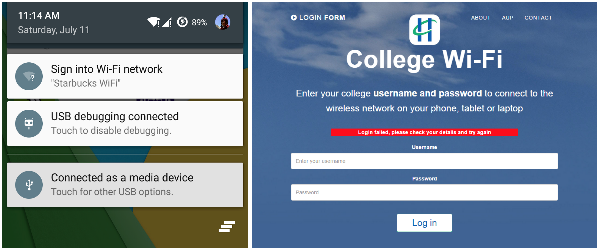
\includegraphics[width=0.75\linewidth]{./2_SensadoCol/Img/CaptivePortals.png}
\end{center}
\caption{Ejemplo de página Web que permite el acceso a Internet a través de WiFi}
\label{PortalesEjemplo}
\end{figure}
 
La solución propuesta en este TFG trataría de aunar la necesidad de monitorización de infraestructuras de la empresa y el acceso a Internet de sus usuarios, implementando un servicio de portal cautivo dotado de una aplicación web con la que se adquieren datos de los sensores del dispositivo en lugar de la clásica introducción manual de datos o credenciales a cambio de la obtención del acceso a la red.

Este sensado colaborativo podría utilizarse para diversas estadísticas (evolución temporal, mapeos de niveles...) con los que la empresa podía obtener una realimentación con unos niveles mínimos de fiabilidad. Los datos recabados no tendrían la misma calidad que el sensado realizado por equipamiento específico de alto rendimiento, pero el coste sería menor y su mantenimiento y configuración más sencillos de realizar. Además, esta solución software tendría una alta escalabilidad y versatilidad de configuraciones, por ejemplo pudiendo permitir el acceso a Internet a cambio de obtención de datos en intervalos regulares en los que el portal cautivo debe mantenerse abierto en alguna ventana o pestaña del navegador, cortándose el acceso si se cierra, o dando un tiempo de acceso fijo (\emph{lease-time}) a cambio de una lectura del micrófono durante un intervalo de tiempo limitado.

\subsection{Idea básica del sistema propuesto}

Como se ha mencionado en el apartado anterior, las soluciones de portal cautivo empleadas habitualmente requieren que el usuario del servicio introduzca manualmente ciertos datos personales o credenciales o que seleccione y visualice publicidad en procesos a menudo tediosos, repetitivos o confusos. El estilo de vida actual, en su búsqueda de la inmediatez, favorece y recompensa las soluciones en las que el usuario pierde el menor tiempo posible en el proceso de acceso al servicio.

Por ello, un servicio de portal cautivo que solo requiera del sensado del dispositivo solo precisaría de la obtención de los permisos pertinentes de acceso al \emph{hardware} ya implementados en los navegadores actuales en forma de popups sencillos con la opción de aceptar o declinar tal acceso. De esta forma e incluso aunque el servicio de portal cautivo utilizado requiera de credenciales, su obtención y el subsiguiente acceso a Internet se hace de una forma mucho más rápida para el usuario, solo teniendo que aceptar y dar permiso a la aplicación web para llevar a cabo el procedimiento automáticamente (la primera vez que la utiliza en un local determinado). En la Figura \ref{LocationMicPermissions} se muestran dos ejemplos típicos de ventanas en la que se solicita permiso al usuario para que el sistema operativo (o navegador) pueda utilizar datos de los sensores del teléfono móvil.

\begin{figure}[!t]
\begin{center}
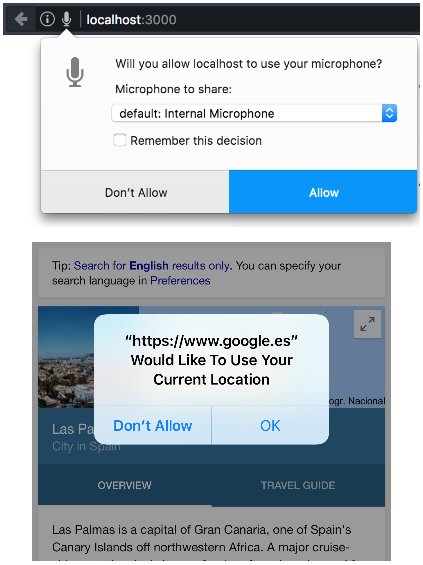
\includegraphics[width=0.5\linewidth]{./2_SensadoCol/Img/LocationMicPermissions.png}
\end{center}
\caption{Ejemplo de ventanas que solicitan permisos para usar sensores del teléfono móvil}
\label{LocationMicPermissions}
\end{figure}

Una implantación que acometa este sistema puede desarrollarse de diversas formas. En el caso de la que concierne a este TFG, se ha optado por utilizar una Raspberry Pi 3 como elemento principal del diseño (en el capítulo 4 se presenta con mayor detalle). En ella se instala todo el \emph{software} necesario para proporcionar el servicio. Se utiliza el modelo 3 de la RaspBerry Pi porque es el primero que cuenta con módulo WiFi integrado en el dispositivo, a diferencia de modelos anteriores en los que había que instalar un módulo USB aparte. En la figura \ref{SystemScheme} se muestra el esquema hardware general planteado, en el que se observa que con la interfaz WiFi de la RaspBerry Pi 3 permitimos que los usuarios se conecten al encaminador que proporciona acceso a Internet de forma controlada.

\begin{figure}[!t]
\begin{center}
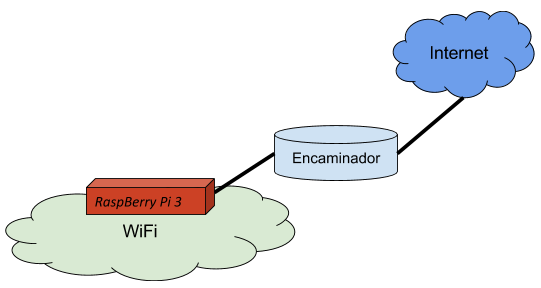
\includegraphics[width=0.75\linewidth]{./2_SensadoCol/Img/SystemScheme.png}
\end{center}
\caption{Esquema general de la infraestructura para proporcionar acceso a Internet mediante una aplicación de sensado móvil colaborativo}
\label{SystemScheme}
\end{figure}

La idea básica de la funcionalidad del sistema de sensado móvil colaborativo implantado es que aquel usuario que desee acceder a Internet, estando en la instalación de un centro que lo permita a través de su WiFi, simplemente permitiría (una sola vez) el uso del micrófono de su teléfono móvil para sensar ruido o sonido que le rodea. A cambio obtiene unos minutos de acceso gratuito a Internet. De esta forma simplificamos el proceso típico de acceder a un portal cautivo con complejos procesos de autorización (cada vez que se desea acceder a Internet). Esto supone un beneficio adicional para el usuario. Además, el propietario del local puede obtener mapas de ruido o sonido de su local a partir del sensado distribuido que hacen los distintos usuarios. Estamos pues ante un escenario en el que no todos los miembros que colaboran tienen exactamente el mismo objetivo; pero todos obtienen un beneficio en la colaboración: el usuario accede a Internet de forma gratuita, el propietario obtiene mapas de ruido con un \emph{hardware} muy barato.

Hasta donde alcanza nuestro conocimiento, no sabemos de ninguna solución similar a ésta, lo que ahonda en la novedad de este TFG. 
\cleardoublepage
\clearpage
\vspace*{\stretch{2}}%{\fill}
\begin{center}
\begin{minipage}{.75\textwidth}
\section{Tecnologías utilizadas}

Para el correcto funcionamiento de nuestro sistema de sensado móvil colaborativo asimétrico con beneficios dispares es necesario el uso del hardware básico presentado en el capítulo 2 y de un conjunto de aplicaciones software. En este capítulo presentamos una descripción somera de todas las tecnologías utilizadas para el desarrollo del proyecto. % \pagebreak
\end{minipage}
\end{center}
\vspace{\stretch{3}} % \vfill % equivalent to \vspace{\fill}
\clearpage% https://tex.stackexchange.com/questions/70714/center-horizontally-and-vertically-a-block-of-text

\subsection{Introducción}
Como habíamos comentado en el capítulo 2, el hardware que necesita el propietario del local es básicamente una Rapberry Pi 3. Para que el sistema de sensado funcione debemos instalar en la Raspberry Pi 3 software que nos permita definir la funcionalidad del portal cautivo que nos permitiría implantar la aplicación de sensado móvil colaborativo de acceso a Internet. En la Figura \ref{CoovaScheme} se muestra un esquema general del \emph{software} necesario. En concreto instalamos el siguiente:

\begin{figure}[!t]
\begin{center}
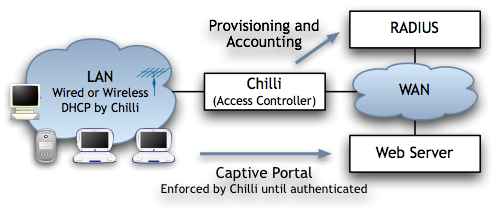
\includegraphics[width=0.75\linewidth]{./3_Tecnologias/Img/CoovaScheme.jpg}
\end{center}
\caption{Esquema general del Software utilizado para la implantación del portal cautivo.}
\source{http://coova.github.io/CoovaChilli/}
\label{CoovaScheme}
\end{figure}

\begin{itemize}
\item \emph{Host Access Point Daemon} (\emph{\acrshort{Hostapd}}) \cite{hostapdDoc}: este daemon de linux se encarga de configurar el módulo WiFi en modo \acrshort{AP}. De esta manera, la Raspberry Pi 3 puede actuar como un punto de acceso configurable, conectándose sus clientes a través de su interfaz \acrshort{WiFi} y obteniendo acceso a la red a través de la interfaz Ethernet de acuerdo al esquema que se muestra en la Figura 2.3.
\item \emph{CoovaChilli} \cite{ChilliGitHub}: el software controlador de acceso que proporcionaría direcciones \emph{Internet Protocol} (\acrshort{IP}) a las conexiones entrantes con su \emph{Dynamic Host Control Protocol} (\acrshort{DHCP}), redirigiría dichas conexiones al portal cautivo para su autenticación en el sistema y las gestionaría junto a un sistema de Autenticación, Autorización y Contabilización (\acrshort{AAA}) que ha de ser instalado aparte, habitualmente un servidor \emph{Remote Authentication Dial-In User Service} (\acrshort{RADIUS}) \cite{RADIUS}.
\item \emph{FreeRADIUS} \cite{FreeRADIUSDoc}: el servicio de \acrshort{AAA} gracias al cual CoovaChilli controla los usuarios del sistema. Para su utilización es necesaria su previa integración con My\acrshort{SQL} \cite{PHPMySQLJavaScript}, que ha de estar instalado en el sistema.
\item \emph{daloRADIUS} \cite{daloRADIUS1}: plataforma Web destinada a controlar el servidor RADIUS de forma gráfica. En este TFG, su contenido es proporcionado por un servidor web.
\item \emph{Node.js}: tecnología JavaScript (para el servidor), complementada con paquetes \acrshort{npm}, con la que implantamos el back-end de nuestra aplicación Web de portal cautivo, que interactuaría con CoovaChilli por medio de su interfaz \acrshort{JSON}.
\item \emph{Front end Web}: página Web a la que acceden los clientes a través de su teléfono móvil implantada en Node.js a partir de: \acrshort{HTML}, \acrshort{CSS} y JavaScript. Esta página Web es el principal elemento diferenciador respecto a otros portales cautivos habituales, dado que su propósito sería el de recopilar del usuario, a través de su navegador, los datos del micrófono del dispositivo conectado al portal cautivo a través de su navegador. Esto es posible gracias a la \emph{Application Programming Interface} (\acrshort{API}) \emph{MediaStream Recording} \cite{MediaStreamRecordingAPI}, tecnología estrechamente relacionada con \emph{\acrshort{WebRTC}} \cite{LibroWebRTC1}.
\end{itemize}

A continuación se realiza un análisis más pormenorizado de las tecnologías utilizadas. Se considera que el lector tiene un conocimiento al menos elemental de las tecnologías Web tradicionales, por lo que estas solo se introducen de forma superficial exceptuando aquellos aspectos concretos que tienen relevancia en este TFG. Los elementos \emph{software} más específicos reciben un análisis pormenorizado, entrando en mayores detalles.

\subsection{\emph{Software} necesario para el funcionamiento básico de la Raspberry Pi 3}
La Raspberry Pi es un tipo de sistema empotrado de pequeño tamaño. Es un computador de un sola placa madre, de reducidas dimensiones. Inicialmente fue planteado como un dispositivo de bajo coste (35 \$) y consumo energético (1.5 W) en su último modelo. Está orientado a propósitos educativos en colegios y países en vías de desarrollo, aunque su uso se extendió rápidamente a otros ámbitos como la robótica. Sus modelos son desarrollados por la Raspberry Pi Foundation en el Reino Unido y actualmente se le considera el ordenador de esa región más vendido.

Desde su introducción en Febrero de 2012 ha habido varias generaciones de este dispositivo, siendo la más reciente la Raspberry Pi 3 Model B que es la usada en este TFG. Este modelo consta de un \emph{Sistema en Chip} (\acrshort{SoC}) de Broadcom, que incluye un procesador quad-core compatible con -\acrshort{ARM}v8 de 64 bits que opera a una frecuencia de 1.2 GHz y un procesador gráfico. Cuenta también con 1GB de \emph{Random Access Memory} (\acrshort{RAM}) \acrshort{LPDDR2} a 900 MHz. Para almacenar el sistema operativo se utiliza una tarjeta \acrshort{MicroSDHC}, y aunque puede instalarse una gran variedad de sistemas operativos diferentes el recomendado es Linux basado en Debian (renombrado como \emph{Raspbian}). En cuanto a entrada-salida la Raspberry Pi 3 cuenta con cuatro puertos \emph{Universal Serial Bus} (\acrshort{USB}), interfaz Ethernet 10/100 Mbps y salidas \emph{High-Definition Multimedia Interface} (\acrshort{HDMI}) y minijack de audio. También incorpora 40 pines entrada-salida de propósito general (\emph{\acrshort{GPIO}, General Purpose Input-Output}) para operaciones a bajo nivel. Otro aspecto de importancia crucial para este TFG es la conectividad inalámbrica, dado que la Raspberry Pi 3 incorpora chipsets \acrshort{WiFi} (versión \acrshort{IEEE} 802.11n) para 2.4 GHz a 150 Mbps y Bluetooth 4.1 a 24 Mbps. Además de esto, en la actualidad se fabrica una amplia gama de accesorios destinados a ampliar la funcionalidad de la Raspberry Pi como cámaras de vídeo, interfaces de control de \acrshort{LED}s y sensores y otras placas de expansión.

\subsubsection{Raspbian y WiFi}

El Raspbian es el sistema operativo recomendado por la Raspberry Pi Foundation desde 2015. Está basado en Debian Jessie y fue desarrollado por Mike Thompson y Peter Green poniendo especial énfasis en los procesadores \acrshort{ARM} de bajo rendimiento de la Raspberry Pi. Incluyen Python, Scratch, Java, Sonic Pi, Mathematica entre otros programas relevantes.

Utiliza \emph{Pi Improved Xwindows Environment Lightweight} (\acrshort{PIXEL}) como entorno gráfico de escritorio. Consiste en un entorno de escritorio \emph{Lightweight X11 Desktop Environment} (\acrshort{LXDE}) modificado y el gestor de ventanas Openbox.
La principal característica de la Raspberry Pi 3 para este TFG es su capacidad de manejo de la tecnología WiFi. Esta tecnología especifica el nivel físico y el subnivel de control de acceso al medio (\acrshort{MAC}, \emph{Medium Access Control}). La versión con la que se ha trabajado es la \acrshort{IEEE} 802.11n, que soporta el uso de varias antenas simultáneamente (\emph{\acrshort{MIMO}, Multiple Input Multiple Output}), aprovechando la propagación multitrayecto para aumentar la tasa de transferencia, e incorpora mejoras en seguridad, agregación de trama, técnicas de \emph{beamforming} para optimizar la emisión de señal junto a otros aspectos. Aunque \acrshort{IEEE} 802.11n también permite trabajar en la frecuencia de 5 GHz, el dispositivo que hemos utilizado como punto de acceso \acrshort{WiFi} trabajaba en 2.4 GHz.

\subsubsection{Hostapd}

Es una utilidad software cuya funcionalidad es transformar las interfaces de red en puntos de acceso y servidores de autenticación. Implementa la gestión de puntos de acceso \acrshort{IEEE} 802.11, autenticación \acrshort{IEEE} 802.11X, \emph{\acrshort{WiFi} Protected Access} (WPA), \acrshort{WPA2}, \emph{Extensible Authentication Protocol} (\acrshort{EAP}), cliente \acrshort{RADIUS}, servidor \acrshort{EAP} y servidor de autenticación \acrshort{RADIUS}. Soporta interfaces con drivers presentes en sistemas Linux y FreeBSD.

Como \emph{daemon} ha sido diseñado para operar en segundo plano como componente \emph{back-end}, soportando aplicaciones front-end separadas. Ha sido programado para funcionar de forma modular por medio de código C organizado en archivos separados. En la Figura \ref{hostapd} se muestra un esquema de la organización del funcionamiento de \acrshort{Hostapd}.

\begin{figure}[!t]
\begin{center}
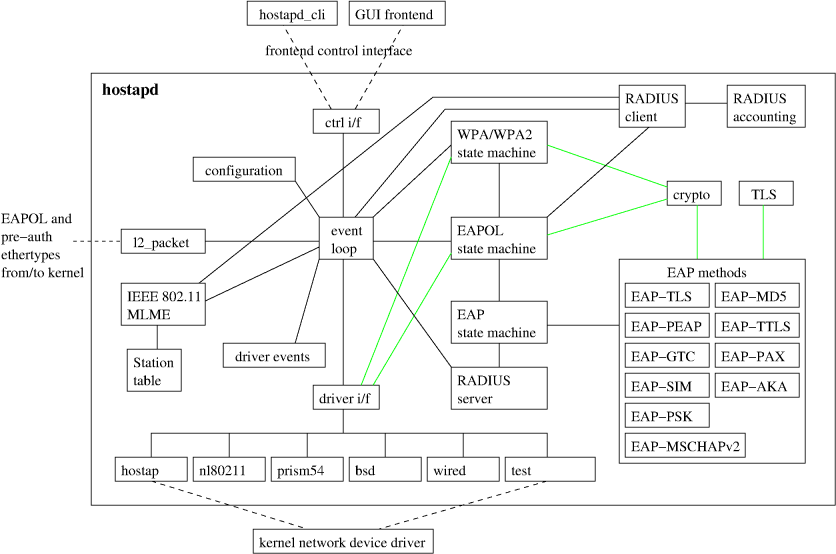
\includegraphics[width=0.75\linewidth]{./3_Tecnologias/Img/hostapd.png}
\end{center}
\caption{Esquema general del funcionamiento de Hostapd.}
\source{http://w1.fi/wpa\_supplicant/devel/}
\label{hostapd}
\end{figure}

El hostapd se configura por medio de un archivo de texto que lista todos los parámetros de configuración, alojado en el archivo \emph{/etc/hostapd/hostapd.conf}, que cuenta con los siguientes atributos relevantes y comúnmente utilizados, entre otros:
\begin{itemize}
\item Atributos de Interfaz Inalámbrica:
\begin{itemize}
\item \emph{interface}: interfaz inalámbrica va a utilizarse.
\item \emph{bridge}: interfaz puente si la interfaz inalámbrica es parte de ella.
\item \emph{driver} (controlador utilizado): suele ser n18011.
\end{itemize}
\item Atributos de Entorno Inalámbrico:
\begin{itemize}
\item \emph{ssid}: nombre o \emph{Service Set IDentifier} (\acrshort{SSID}) de la red que aparecería en la lista de redes disponibles al hacer la habitual búsqueda de red desde un dispositivo inalámbrico.
\item \emph{hw\_mode}: fija el modo de operación de la interfaz y los canales permitidos. Los valores permitidos dependen del hardware pero siempre son un subconjunto de \emph{a}, \emph{b} o \emph{g}. Aunque se configure una red \acrshort{IEEE} 802.11n no es aquí donde debe indicarse, ya que \acrshort{IEEE} 802.11n opera sobre la funcionalidad de \acrshort{IEEE} 802.11a o \acrshort{IEEE} 802.11g.
\item \emph{channel}: el canal en el que hostapd operaría como punto de acceso. Debe ser un canal soportado por el modo de hardware establecido en el atributo \emph{hw\_mode}. Los canales de \acrshort{IEEE} 802.11 son de 20 MHz de anchura (4 canales) en el espectro, solapándose entre ellos, por lo que deben escogerse de forma que esto no suceda. Por ejemplo, si la mayoría de puntos de acceso de la red utilizan el canal 6 sería óptimo utilizar el canal 1 o el canal 11 para evitar interferencias por solapamiento.
\end{itemize}
\item Atributos de \acrshort{IEEE} 802.11n:
\begin{itemize}
\item \emph{ieee80211n}: atributo booleano que al asignársele el valor 1 activa las funcionalidades propias de \acrshort{IEEE} 802.11n.
\item \emph{ht\_capab}: lista de las capacidades \acrshort{IEEE} 802.11n soportadas por el dispositivo utilizado. Actúan como flags, activándose al ser escritos entre corchetes. Ejemplos de ello serían habilitar el uso de canales de 40 MHz (\emph{[HT40+]}) o activar el modo \acrshort{DSSS}/\acrshort{CCK} en dichos canales (\emph{[DSSS\_CCK-40]}).
\end{itemize}
\item Autenticación y cifrado:
\begin{itemize}
\item \emph{macaddr\_acl}: controla el filtrado de direcciones \acrshort{MAC}.
\item \emph{auth\_algs}: campo de bits en el que el primero es para autenticación abierta, el segundo es por autenticación de Clave Compartida (\acrshort{WEP}), pudiendo activar ambos introduciendo un 3.
\item \emph{ignore\_broadcast\_ssid}: activa o desactiva la difusión del \acrshort{SSID}.
\item \emph{wpa}: Un campo de bits como \emph{auth\_algs}. El primero activa \acrshort{WPA}1, el segundo activa \acrshort{WPA2} y el 3 activa los dos.
\item \emph{wpa\_psk} o \emph{wpa\_passphrase}: contraseña para la autenticación \acrshort{WPA}.
\item \emph{wpa\_key\_mgmt}: controla con qué algoritmos de gestión de claves podría autenticarse un cliente.
\item \emph{wpa\_pairwise}: controla el encriptado de datos de \acrshort{WPA}.
\item \emph{rsn\_pairwise}: controla el encriptado de datos de \acrshort{WPA2}.
\end{itemize}
\end{itemize}

En el bloque de código \ref{HostapdConf1} se muestra un ejemplo de archivo de configuración. 

\begin{listing}[H]
\begin{minted}
[
frame=lines,
framesep=2mm,
baselinestretch=1.2,
bgcolor=lightgray,
fontsize=\footnotesize,
breaklines=true,
breaksymbolleft={}
]
{bash}
interface=wlan0
driver=nl80211
ssid=RaspAP
hw_mode=g
channel=8
wpa=2
wpa_psk=928519398acf811e96f5dcac68a11d6aa876140599be3dd49612e760a2aaac0e
wpa_key_mgmt=WPA-PSK
wpa_pairwise=CCMP
rsn_pairwise=CCMP
beacon_int=100
auth_algs=3
wmm_enabled=1
\end{minted}
\caption{Ejemplo de archivo de configuración de Hostapd}
\label{HostapdConf1}
\end{listing}

\subsection{El Servidor RADIUS}

CoovaChilli hace uso de servicios de \acrshort{AAA} separados para poder funcionar. Habitualmente este servicio es un servidor \acrshort{RADIUS} instalado de forma separada. Por ello, se exponen algunos detalles de su funcionamiento, junto a detalles la solución concreta de servidor \acrshort{RADIUS} utilizada en este TFG, FreeRADIUS, y otros aspectos relevantes.

RADIUS es un protocolo cliente/servidor que proporciona gestión de AAA de forma centralizada para aquellos clientes de un servicio de Red. Fue desarrollado en 1991 por parte de Livingston Enterprises, Inc. como un protocolo de autenticación y contabilidad para servidores de acceso, convirtiéndose en un estándar de la \emph{Internet Engineering Task Force} (\acrshort{IETF}). Se implanta a nivel de aplicación y puede utilizar tanto \emph{Transmission Control Protocol} (\acrshort{TCP}) como \emph{User Datagram Protocol} (\acrshort{UDP}). \acrshort{RADIUS} suele ser el back-end para autenticaciones de \acrshort{IEEE} 802.11x, como un proceso en segundo plano ejecutándose en un servidor UNIX o Windows. Actualmente se utiliza de forma prácticamente masiva por proveedores de servicios de Internet para gestionar el acceso al mismo o a redes internas, inalámbricas y a servicios de correo electrónico.

\subsubsection{El Servidor RADIUS}

La autenticación y autorización de RADIUS es la descrita en la \emph{Request For Comments} (\acrshort{RFC}) 2865 mientras que la contabilidad es la descrita en la \acrshort{RFC} 2866.

Para la autenticación y autorización, el cliente envía una petición al \emph{Servidor de Acceso a la Red} (\acrshort{NAS}) para obtener acceso a un recurso de red particular utilizando credenciales de acceso. Estas credenciales llegan a este dispositivo mediante los protocolos de nivel de enlace. En respuesta, el \acrshort{NAS} envía un mensaje RADIUS de Petición de Acceso al servidor RADIUS, pidiendo autorización para conceder el acceso mediante el protocolo \acrshort{RADIUS}. Esta petición incluye credenciales de acceso, habitualmente un nombre de usuario y contraseña o un certificado de seguridad proporcionados por el usuario. El servidor RADIUS comprueba que la información es correcta utilizando patrones de autenticación como \emph{Password Authentication Protocol} (\acrshort{PAP}), \emph{Challenge-Handshake Authentication Protocol} (\acrshort{CHAP}) o \acrshort{EAP}. En este punto se verifica la información de identificación con las almacenadas en un archivo del servidor o una fuente externa, como una base de datos \acrshort{SQL}. Tras esto, el servidor \acrshort{RADIUS} puede responder de tres formas (Figura \ref{RADIUSAccept}):

\begin{itemize}
\item \emph{Access Accept}: se concede acceso al usuario.
\item \emph{Access Challenge}: solicita información adicional, como una contraseña secundaria o un PIN.
\item \emph{Access Reject}: se deniega el acceso a todos los recursos de red solicitados por el usuario.
\end{itemize}

\begin{figure}[!t]
\begin{center}

\includegraphics[width=0.75\linewidth]{./3_Tecnologias/Img/RADIUSAccept.png}
\end{center}
\caption{Ejemplo de mensajes de aceptación de RADIUS.}
\source{https://en.wikipedia.org/wiki/RADIUS}
\label{RADIUSAccept}
\end{figure}

Estas tres respuestas RADIUS pueden incluir atributos de mensaje que pueden dar una razón para el rechazo, la petición de la información adicional (\emph{Access Challenge}) o un mensaje de bienvenida.

Los atributos de autorización se entregan al NAS especificando los términos de acceso. Por ejemplo, una respuesta \emph{Access Accept} podría incluir los siguientes atributos:

\begin{itemize}
\item IP específicas o subconjunto de IP posibles a ser asignadas al usuario.
\item Un tiempo máximo de conexión.
\item Lista de prioridades u otras restricciones de acceso para el usuario.
\item Parámetros de Calidad de Servicio (\acrshort{QoS}).
\end{itemize}

\subsubsection{Contabilidad}
Cuando se proporciona acceso al usuario el NAS envía un mensaje de \emph{Accounting Start} (un paquete de petición de contabilidad RADIUS que contiene un atributo \emph{acct\_status\_type} con el valor \emph{start}) para señalizar el comienzo del acceso a la red. Este registro normalmente contiene el identificador de usuario, dirección de red y un identificador de sesión único.

De forma periódica el NAS puede enviar al servidor RADIUS unos registros \emph{Interim Update} (un paquete similar al \emph{Accounting Start} pero con el valor de \emph{acct\_status\_type} establecido como \emph{interim-update}) para actualizar el estado de la sesión. Estos registros suelen contener la duración actual de la sesión y otra información sobre el uso de datos (Figura \ref{RADIUSCont}).

\begin{figure}[!t]
\begin{center}

\includegraphics[width=0.75\linewidth]{./3_Tecnologias/Img/RADIUSCont.png}
\end{center}
\caption{Ejemplo de mensajes de contabilidad en RADIUS.}
\source{https://en.wikipedia.org/wiki/RADIUS}
\label{RADIUSCont}
\end{figure}

Cuando el acceso a la red del usuario se cierra el NAS envía un registro de Accounting Stop (similar a lo anterior, \emph{acct\_status\_type} fijado en stop) al servidor RADIUS, proporcionando información de la duración final de uso en términos de tiempo, paquetes transferidos, datos transferidos, razón de la desconexión y otra información relacionada con el acceso a la red.

El propósito de estos datos es principalmente para facturar al cliente de forma adecuada, aunque también se usa para propósitos estadísticos o de monitorización de red. Todos estos mensajes suelen contar con su propio sistema de mensajes de reconocimiento (\emph{acknowledgement, ack}), reintentando los registros de contabilidad a intervalos determinados hasta que dicho \emph{ack} es recibido.

\subsubsection{Seguridad}
El protocolo RADIUS transmite contraseñas ocultas utilizando un secreto compartido y el algoritmo de hash MD5. Para aumentar aún más la protección del tráfico RADIUS pueden utilizarse medidas adicionales como túneles IPsec. Solo las credenciales de usuario son protegidas por RADIUS, otra información que pasa a través de este podría ser susceptible a efectos de seguridad. Algunas medidas para solucionar estos problemas pueden encontrarse en el protocolo RadSec, con el que se transportan los datagramas RADIUS mediante TCP y \emph{Transport Layer Security} (\acrshort{TLS}).

\subsubsection{FreeRADIUS}

Aunque habitualmente se utilice este nombre para referirse tan solo al servidor, FreeRADIUS es realmente una suite gratuita de RADIUS distribuida bajo la \acrshort{GPL}, version 2, en descarga y uso gratuitos. Su desarrollo comenzó en Agosto de 1999 por Alan DeKok y Miquel van Smoorenburg utilizando un diseño modular para animar la participación de la comunidad. Incluye dicho servidor RADIUS, una biblioteca de clientes RADIUS con licencia basada en \emph{Berkeley Software Distribution} (\acrshort{BSD}), una biblioteca \emph{Pluggable Authentication Module} (\acrshort{PAM}), un módulo Apache y otras utilidades relacionadas con RADIUS. Es rápido, modular, escalable y con una gran cantidad de opciones. En la actualidad se encuentra en su versión 3, que incluye soporte para RADIUS sobre TLS incluyendo RadSec.

Es el servidor RADIUS de código abierto más popular y el servidor RADIUS más desplegado en el mundo con una base de usuarios estimada en más de 100 millones según una encuesta de 2006 citada en la Web del proyecto. Soporta todos los protocolos de autenticación habituales y el servidor cuenta con una herramienta Web para la administración de usuarios basada en PHP llamada \emph{Dialup Admin}. Es la base de muchos productos y servicios RADIUS comerciales, como sistemas embebidos o WiMAX. Proporciona servicios de \emph{Authentication, Authorization and Accounting} (AAA) a numerosas empresas de envergadura, compañías de telecomunicaciones y proveedores de servicios de internet de Tier 1 (como podrían ser AT\&T, Orange o Telefónica). También se usa en la comunidad académica, incluyendo \emph{eduroam}, que lo implementa junto a RadSec para incrementar la seguridad.

Los módulos incluidos en el núcleo del servidor soportan bases de datos MySQL, PostgreSQL y Oracle entre otros. También soportan todos los tipos de autenticación \emph{Extensible Authentication Protocol} (EAP) populares, como \emph{Protected EAP} (\acrshort{PEAP}) y \emph{EAP Tunneled Transport Layer Security} (\acrshort{EAP-TTLS}). Tiene incluidos más de 100 diccionarios de fabricantes, asegurando su compatibilidad con una amplia gama de dispositivos \emph{Network Access Server} (NAS).

Desde su versión 2 tiene soporte de \emph{hosting} virtual, \emph{IPv6} y \emph{Virtual Local Area Network Management Policy Server} (VMPS).

Existen varias herramientas para gestionar FreeRADIUS aparte de la ya mencionada Dialup Admin. En este TFG se utiliza la solución daloRADIUS, una aplicación basada en Web orientada a la gestión de hotspots y despliegues de proveedores de servicios de Internet. Cuenta con una interfaz sencilla, informes gráficos, contabilidad, procesos de facturación y se integra con Google Maps para geolocalización. El aspecto general de esta interfaz de usuario se muestra en la Figura \ref{daloRADIUS1}.

\begin{figure}[!t]
\begin{center}
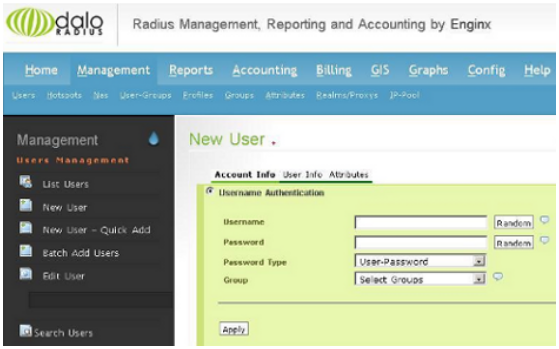
\includegraphics[width=0.75\linewidth]{./3_Tecnologias/Img/daloRADIUS1.png}
\end{center}
\caption{Pantalla de adición de nuevo usuario.}
\label{daloRADIUS1}
\end{figure}

\subsection{CovaChilli}
CoovaChilli es un \emph{software} controlador de acceso WiFi a Internet de código abierto basado en el antiguo proyecto ChilliSpot, ya abandonado. Lanzado bajo \emph{GNU General Public License} (GPL), en la actualidad es mantenido por los aportes de personal original de ChilliSpot. CoovaChilli carece de interfaz gráfica, por lo que ha de controlarse utilizando la orden chilli en el terminal. Proporciona un entorno de portal cautivo y utiliza RADIUS o \emph{Hyper Text Transfer Protocol} (\acrshort{HTTP}) para proporcionar acceso y contabilidad. CoovaChilli es parte integral de CoovaAP, un firmware basado en OpenWRT especializado en \emph{hotspots}. Soporta dos métodos de acceso diferentes para una red local inalámbrica: \emph{Universal Access Method} (\acrshort{UAM}) y WPA.

\subsubsection{Funcionamiento}
Utiliza mediante tres interfaces principales:

\begin{itemize}
\item De enlace descendente (\emph{downlink}) que acepta conexiones de los clientes, mediante DHCP y ARP. Los clientes pueden encontrarse en dos estados: no autenticados y autenticadas. En este último caso, sus peticiones Web son redirigidas a un portal cautivo, el servidor Web de autenticación que usualmente les solicita usuario y contraseña. El servidor Web envía las credenciales del usuario al proceso chilli mediante redirecciones del navegador.  
\item De RADIUS para autenticar a los clientes. Para el método de acceso UAM se utilizan desafíos y contraseñas CHAP de acuerdo a la RFC 2865. Para la autenticación por WPA se utiliza el atributo de mensaje EAP para RADIUS de acuerdo a la RFC 2869. Los atributos de mensaje descritos en la RFC 2548 se usan para transferir claves de cifrado desde el servidor RADIUS hacia CoovaChilli. Si la autenticación tiene éxito el estado del cliente pasa a ser de autenticado. 
\item De enlace ascendente (\emph{uplink}) para dirigir el tráfico hacia otras redes. 
\end{itemize}

La interfaz de enlace ascendente se implementa utilizando drivers \emph{network tunnel} (\acrshort{TUN}) que opera con el encaminamiento de datagramas IP y network \acrshort{TAP} que opera a nivel de puente (\emph{bridge}) con datagramas de nivel de enlace (normalmente Ethernet). TUN/TAP funcionan como dispositivos de comunicación virtuales del núcleo del sistema operativo encargados de recoger datos del nivel de aplicación y enviarlos a la Red y viceversa. Cuando el proceso \emph{chilli} comienza se habilita una interfaz TUN y se llama a un \emph{script} de configuración externo opcional. Esto es, las interfaces TUN/TAP son interfaces \emph{software}, solo existen en el núcleo del sistema y se utilizan para realizar funciones de red a nivel de espacio de usuario. Una vez implantadas actúan como cualquier otra interfaz del sistema. Se les pueden asignar direcciones IP, su tráfico puede ser analizado, se puede determinar qué caminos le apuntan, añadirles directivas de cortafuegos...

\subsubsection{Configuración}

El archivo principal de CoovaChilli es  \emph{/usr/local/etc/chilli.conf} el cual incluye otros tres: \emph{main.conf}, \emph{hs.conf} y \emph{local.conf}. Los dos primeros son creados por los scripts del shell existentes en el archivo \emph{functions} basándose en las configuraciones de otros archivos mencionados a continuación y obteniendo algunas configuraciones del servidor RADIUS y otras \acrshort{URL}. El archivo \emph{local.conf} está reservado para configuraciones de lugares específicos.
Las configuraciones por defecto que son establecidas en \emph{chilli.conf} se encuentran en \emph{/usr/local/etc/chilli/defaults}. Los valores existentes en este último archivo pueden sobreescribirse durante la inicialización de chilli si existe otro archivo en \emph{/usr/local/etc/chilli/config}, que no es más que una copia del archivo defaults sobrescribiendo los valores de los atributos que se desea cambiar.
Cada vez que se enciende el dispositivo en el que está instalado CoovaChilli, el script presente en \emph{/usr/local/etc/init.d/chilli} se ejecuta tomando las configuraciones de los archivos \emph{defaults} y \emph{config} mencionados anteriormente, ejecutando también el script \emph{/usr/local/etc/chilli/functions} para asistir en esta configuración y la de otros archivos relevantes para el funcionamiento del programa, creando de este modo los respectivos archivos \emph{main.conf}, \emph{hs.conf} y \emph{local.conf}.

Adicionalmente, CoovaChilli implementa un servidor Web mínimo destinado a servir contenido en el directorio \emph{/etc/local/etc/chilli/www/}, lugar en el que puede ubicarse un servicio de portal cautivo sencillo. Por defecto, en este directorio se implementa un portal cautivo con pantalla de espera que redirige a un formulario ensamblado con plantillas HTML y archivos de Web scripts \emph{Common Gateway Interface} (\acrshort{CGI}) para contenido dinámico. Estos archivos (con la extensión .chi) son procesados con el software Haserl \cite{Haserl}, por lo que si se usa la configuración por defecto de CoovaChilli este programa ha de estar instalado.

Aunque CoovaChilli cuenta con numerosas opciones, en este TFG se usa y modifica tan solo un subconjunto de ellas, asignándoles valores en los archivos \emph{defaults} y \emph{config}:

\begin{itemize}
\item \emph{HS\_WANIF}: especifica la interfaz de red que cuenta con acceso a internet, habitualmente la interfaz Ethernet del dispositivo, \emph{eth0}.
\item \emph{HS\_LANIF}: interfaz a la que se conectan los clientes, habitualmente la interfaz WiFi del dispositivo, \emph{wlan0}.
\item \emph{HS\_NETWORK}: dirección IP de la red a la que se conectan los clientes, por ejemplo 192.160.10.0. Habitualmente esta dirección es la determinada al configurar una IP estática para \emph{wlan0} en el archivo \emph{/etc/network/interfaces} del sistema operativo.
\item \emph{HS\_UAMLISTEN}: la IP del dispositivo de red al que se conectan los clientes. Por supuesto, debe pertenecer al rango IP de la red especificada en el atributo anterior, siguiendo el ejemplo dicha IP sería 192.168.10.1.
\item \emph{HS\_UAMALLOW}: redes y dominios en los que los usuarios no autenticados sí tienen permitida la navegación. Habitualmente solo se permite la red local desde la que también se serviría el portal cautivo (el mismo valor que el atributo \emph{HS\_NETWORK}), aunque para otros servicios de portal cautivo más avanzados podría permitirse el acceso a otros dominios, por ejemplo a la URL de la correspondiente API de Facebook para la autenticación por esta red social o al dominio de PayPal para realizar pagos de tarifas.
\item \emph{HS\_UAMSECRET}: clave secreta con la que se cifran las credenciales que se envíen desde el servidor Web del portal cautivo hacia CoovaChilli.
\item \emph{HS\_UAMFORMAT}: ubicación y puerto del servidor Web que proporcionaría el portal cautivo.
\item \emph{HS\_UAMHOMEPAGE}: ubicación y puerto a la que se redirigirían las peticiones Web de los clientes al conectarse a la red. Habitualmente, esto es una página de bienvenida que luego redirige hacia el contenido servido en la ubicación especificada en \emph{HS\_UAMFORMAT}.
\item \emph{HS\_SSID}: SSID de la red.
\end{itemize}

\subsubsection{Interfaz \emph{JavaScript Object Notation}}

\emph{JavaScript Object Notation} (JSON) es perfil de transmición de datos desde un servidor Web a un navegador. Tiene menos datos de cabecera que el \emph{Xtensible Markup Language} (\acrshort{XML}) habitualmente utilizado en \emph{Asynchronous JavaScript And XML}(\acrshort{AJAX}) y otros servicios y por ello se ha considerado una alternativa a este y ha alcanzado gran popularidad. CoovaChilli usa JSON para realizar el control de usuarios de forma que pueda utilizarse un portal cautivo de cualquier tipo e incluso en servidores distintos al incorporado en el programa a los que pueda acceder el cliente, previa habilitación del acceso al dominio correspondiente en el atributo \emph{HS\_UAMALLOW} del archivo de configuración. Un usuario puede autenticarse a través de ella, obtener el estado de su conexión o desconectarse del portal cautivo.

Para comunicarse con la interfaz JSON de CoovaChilli se utiliza una biblioteca JavaScript, instalada por defecto en \emph{/usr/local/etc/chilli/www/ChilliLibrary.js}. Esta biblioteca crea el objeto global \emph{chilliController}, que ha de inicializarse con los valores necesarios según nuestra configuración. El portal cautivo que se implemente pasa a utilizar los métodos expuestos por el objeto \emph{chilliController} para comunicarse con CoovaChilli, enviándole peticiones HTTP GET a este y recibiendo respuestas en el formato JSON.

El objeto \emph{chilliController} puede enviar los siguientes órdenes a CoovaChilli:

\begin{itemize}
\item \emph{logon}: intenta un login utilizando CHAP. La respuesta contendría los datos de sesión y los datos iniciales de contabilidad. Es llamado mediante el método \emph{logon(username, password)}.
\item \emph{logoff}: termina la sesión actual. Es llamado mediante el método \emph{logoff()}.
\item \emph{status}: proporciona los datos de contabilidad más recientes. Es llamado mediante el método \emph{refresh()}.
\end{itemize}


Cuando un cliente es autorizado, el objeto \emph{chilliController} consulta periódicamente la información de contabilidad, enviando órdenes de \emph{status} para actualizar los datos (orden \emph{autorefresh}).
CoovaChilli facilita una plantilla de código en su página Web que puede alojarse en el HTML de un portal cautivo que utilice esta interfaz (Bloque de código \ref{JSONTemplate}).

\begin{listing}[H]
\begin{minted}
[
frame=lines,
framesep=2mm,
baselinestretch=1.2,
bgcolor=lightgray,
fontsize=\footnotesize,
breaklines=true,
breaksymbolleft={}
]
{html}
<script src="http://my.host.com/ChilliLibrary.js"></script>
<script>
// The included script creates a global chilliController object
// If you use non standard configuration, define your configuration 
  chilliController.host = "10.0.0.1";  // Default is 192.168.182.1
  chilliController.port  = 4003     ; //  Default is 3990
  chilliController.interval = 60    ; // Default is 30 seconds
  
// then define event handler functions
  chilliController.onError  = handleErrors;
  chilliController.onUpdate = updateUI ;

// when the reply is ready, this handler function is called
  function updateUI( cmd ) {
    alert ( 'You called the method' + cmd +
      '\n Your current state is =' + chilliController.clientState ) ;
  }
  
// If an error occurs, this handler will be called instead
  function handleErrors ( code ) {
    alert ( 'The last contact with the Controller failed. Error code =' + code );
  }
//  finally, get current state
  chilliController.refresh();
</script>

\end{minted}
\caption{Plantilla de código de CoovaChilli para el manejo de la interfaz JSON}
\label{JSONTemplate}
\end{listing}

El \emph{chilliController} es un objeto global creado por el script incluido al principio. Por defecto, está configurado para contactar con CoovaChilli en 192.168.182.1:3990 cada 30 segundos. Si deseamos valores diferentes, pueden modificarse antes de llamar a cualquier método tal y como se ve en el bloque de código. Tras configurar el objeto \emph{chilliController} se debe llamar al método \emph{refresh()} para determinar el estado actual del cliente.

CoovaChilli ha implementado los siguientes atributos para el objeto ChilliController. Al ser una interfaz que continúa expandiéndose y desarrollándose existen otros atributos aún no implementados pero presentes en la documentación que se han omitido en este TFG.

\begin{itemize}
\item \emph{host}: la dirección IP del controlador de acceso de CoovaChilli.
\item \emph{port}: el puerto HTTP para las peticiones JSON.
\item \emph{interval}: intervalo medido en segundos. Mientras el usuario está autenticado, los datos de contabilidad y de sesión se actualizan mediante \emph{polling} a CoovaChilli a este intervalo.
\item \emph{language}: el idioma preferido para el mensaje de respuesta (código de idioma de dos letras ISO, por ejemplo ‘en’).
\item \emph{clientState}: estado del terminal. \emph{UNKNOWN} significa que aún no se ha recibido información desde CoovaChilli. Otros valores posibles son \emph{NOT\_AUTHORIZED}, \emph{AUTHORIZED} y \emph{AUTH\_PENDING}.
\item \emph{command}: el último comando enviado a CoovaChilli (que podría estar pendiente): \emph{logon, logoff, refresh, autorefresh}.
\item \emph{sessionId}: identificador único de sesión generado por CoovaChilli (\emph{Acct-Session-Id}). Se utiliza para asegurar que las propiedades del miembro de la sesión y el miembro de la contabilidad pertenezcan a la misma sesión.
\item \emph{message}: mensaje a ser mostrado al usuario. Puede ser el Mensaje Respuesta RADIUS o un mensaje generado por CoovaChilli.
\item \emph{redir}: este atributo expone datos leídos en la URL de la redirección inicial que se realiza hacia el portal cautivo indicado en el atributo de configuración de \emph{HS\_UAMHOMEPAGE}. Solo existe si la página especificada en dicho atributo incluye un script manejador de \emph{chilliController}.
\item \emph{originalURL}: URL pedida originalmente por el cliente antes de su redirección.
\item \emph{redirectionURL}: URL a la que se va a redirigir a continuación.
\item \emph{macAddress}: atributo RADIUS \emph{Calling-Station-Id}. La dirección MAC del dispositivo cliente.
\item \emph{ipAddress}: atributo RADIUS \emph{Framed-IP-Address}.
\item \emph{location}: este atributo contiene información básica sobre la ubicación.
\item \emph{name}: atributo RADIUS \emph{WISPr-Location-Name}, el nombre de la ubicación también almacenada en el atributo locationname o radiuslocationname de chilli.conf.
\item \emph{session}: expone los atributos RADIUS recibidos en el paquete RADIUS \emph{access-attempt}. Estos atributos son fijos durante una sesión.
\item \emph{startTime}: el momento de inicio de sesión de CoovaChilli. Es un objeto Date de ECMAScript. No es un atributo RADIUS.
\item \emph{sessionTimeout}: temporizador para la finalización de sesión.
\item \emph{idleTimeout}: temporizador para el tiempo de inactividad.
\item \emph{accounting}: valores de contabilidad de Volumen/Tiempo. Van cambiando durante la sesión.
\item \emph{sessionTime}: atributo RADIUS \emph{Acct-Session-Time}. La duración de la sesión.
\item \emph{idleTime}: tiempo de inactividad calculado por CoovaChilli (el tráfico desde o hacia CoovaChilli es ignorado). No es un atributo RADIUS, pero el objeto controlador lo utiliza para planificar la siguiente actualización de datos tras una desconexión por IdleTimeout.
\item \emph{inputOctets}: atributo RADIUS \emph{Acct-Input-Octets}.
\item \emph{outputOctets}: atributo RADIUS \emph{Acct-Output-Octets}.
\item \emph{inputGigawords}: atributo RADIUS \emph{Acct-Input-Gigawords}.
\item \emph{outputGigawords}: atributo RADIUS \emph{Acct-Output-Gigawords}.
\end{itemize}

CoovaChilli ha implementado los siguientes manejadores de eventos:

\begin{itemize}
\item \emph{onUpdate}: función llamada cuando el objeto chilliController se actualiza. Las actualizaciones ocurren cuando nuevos datos se reciben desde el controlador. Esto puede ocurrir después de que un método se llame explícitamente (\emph{logon, logoff, refresh}) o automáticamente a intervalos determinados por el atributo interval, cuando se autoriza al cliente (\emph{autorefresh}). La función recibe el nombre de la orden que causó la actualización como argumento.
\item \emph{onError}: función llamada cuando no puede obtenerse una respuesta JSON correcta del controlador (se ha caído el enlace inalámbrico, la sintaxis JSON es incorrecta…). La función recibe un código de error como argumento.
\end{itemize}

Como se ha mencionado anteriormente, los órdenes se envían a CoovaChilli mediante peticiones HTTP. El parámetro GET \emph{lang} se usa en \emph{logon} para pasar el idioma preferido. El campo \emph{version} se utiliza para controlar las diferentes versiones del protocolo JSON de CoovaChilli. Si un parámetro para hacer \emph{callbacks} existe, CoovaChilli pone el texto de salida JSON entre paréntesis y lo adjunta con la función de \emph{callback}. La salida sería como una llamada a una función con el objeto JSON pasado como parámetro.

Para el logon, siguiendo el ejemplo del bloque de código que configuró el objeto chilliController en apartados anteriores, cuando se llama al método \emph{logon()} del Controlador el objeto genera un desafío CHAP aleatorio (string hexadecimal) y realiza la petición a la \acrshort{URL} \emph{http://192.168.182.1:3990/json/logon} con las siguientes \emph{strings} de petición: \emph{?username=XXXX\&chapchallenge=YYYY\&chappassword=0123456789abcdef\&lang=EN}.
CoovaChilli responde con un objeto en formato JSON del bloque de código \ref{JSONResponseYES}:

\begin{listing}[H]
\begin{minted}
[
frame=lines,
framesep=2mm,
baselinestretch=1.2,
bgcolor=lightgray,
fontsize=\footnotesize,
breaklines=true,
breaksymbolleft={}
]
{json}
{
  "version" : "1.0",
  "clientState" : 1 ,
  "sessionId" : "4662e92b0000000e" ,
  "message" : "You're now connected" ,
  "location" : {
     "name":  "Coova labs"
  },
 
  "redir" : {
    "macAddress" : "00-30-1B-B5-03-6B",
    "originalURL" : "http://my.yahoo.com/",
    "redirectionURL" : "http://www.coova.org/welcome.php",
    "ipAddress" : "192.168.182.47"
  },
 
  "session" : {
    "startTime" : 137550720,
    "terminateTime" : 13756072,
    "sessionTimeout" : 3600,
    "idleTimeout" : 240,
    "maxInputOctets" : 100000000,
    "maxOutputOctets" : 100000000,
    "maxTotalOctets" : 100000000,
    "bandwidthMaxDown" : 1000000,
    "bandwidthMaxUp" : 1000000
  },
  
  "accounting": {
     "sessionTime" : 2,
     "idleTime" : 0,
     "inputOctets" : 0,
     "outputOctets" : 0,
     "inputGigawords" : 0,
     "outputGigawords" : 0
  }
}
\end{minted}
\caption{Respuesta de la interfaz JSON a un logon()}
\label{JSONResponseYES}
\end{listing}

Si por el contrario la autorización no tiene éxito la respuesta JSON será la que se muestra en el bloque de código \ref{JSONResponseNO}.

\begin{listing}[H]
\begin{minted}
[
frame=lines,
framesep=2mm,
baselinestretch=1.2,
bgcolor=lightgray,
fontsize=\footnotesize,
breaklines=true,
breaksymbolleft={}
]
{json}
{
  "version": "1.0",
  "clientState": 0,
  "message": "This username does not exist",
  "location" : { "name":"My HotSpot" }
 }
\end{minted}
\caption{Respuesta de la interfaz JSON a un logon() fallido}
\label{JSONResponseNO}
\end{listing}

Para el logoff, cuando se llama al método de desconexión se realiza la petición a \emph{http://192.168.182.1:3990/json/logoff?lang=en\&callback=myfunc}. La respuesta JSON pasa a tener esta forma: \emph{myfunc ( { ``version'': ``1.0'', ``clientState'': 0 } )}. 

Para el \emph{Refresh}, cuando se llama al método de actualización se realiza la petición a \emph{http://192.168.182.1:3990/json/status?lang=en}. La respuesta JSON en este caso se muestra en el bloque de código \ref{JSONRefresh1}.

\begin{listing}[H]
\begin{minted}
[
frame=lines,
framesep=2mm,
baselinestretch=1.2,
bgcolor=lightgray,
fontsize=\footnotesize,
breaklines=true,
breaksymbolleft={}
]
{json}
{
 "version" : "1.0",
 "clientState" : 1 ,
 "sessionId" : "4662e92b0000000e" ,
 "accounting": {
     "sessionTime" : 1230,
     "idleTime" : 240,
     "inputOctets" : 2912981 ,
     "outputOctets" : 51498511,
     "inputGigawords" : 0,
     "outputGigawords" : 0
  }
}
\end{minted}
\caption{Respuesta de la interfaz JSON a un refresh()}
\label{JSONRefresh1}
\end{listing}

No es necesario repetir las propiedades fijas de sesión. El atributo \emph{sessionId} se usa para asociar los nuevos valores de contabilidad recibidos con los valores de sesión recibidos con la orden \emph{logon} inicial.

Si el cliente no está autorizado se envía esta respuesta a las peticiones la respuesta sería la del bloque de código \ref{JSONNoAuthorized}.

\begin{listing}[H]
\begin{minted}
[
frame=lines,
framesep=2mm,
baselinestretch=1.2,
bgcolor=lightgray,
fontsize=\footnotesize,
breaklines=true,
breaksymbolleft={}
]
{json}
{
 "version" : "1.0",
 "clientState" : 0
}
\end{minted}
\caption{Respuesta de la interfaz JSON a una petición no autorizada}
\label{JSONNoAuthorized}
\end{listing}

\subsection{El entorno node.js para programación de back-end }

JavaScript junto a HTML y CSS son los tres pilares básicos de la programación \emph{front-end} (cliente). Los servidores (\emph{back-end}), suelen estar programados en otros lenguajes como \emph{Hypertext Preprocessor} (PHP), Java \cite{JavaServer} o Python \cite{Python}... Poco a poco JavaScript se ha convertido en una opción para programar los \emph{back-ends} debido a la aparición de Node.js.  Esto se debe a la iniciativa de intentar unificar todo el desarrollo Web en un único lenguaje de programación introduciendo el  paradigma \emph{JavaScript en todas partes}.

El Node.js tiene una arquitectura dirigida por eventos capaz de manejar la entrada-salida asíncrona, en un esfuerzo por aumentar la escalabilidad y la tasa de transmisión en aplicaciones Web con gran cantidad de operaciones de este tipo o aplicaciones Web en tiempo real. Su funcionalidad se basa en bibliotecas JavaScript conectadas entre ellas y al sistema operativo por medio de \emph{bindings} en C++. Utiliza una combinación del motor JavaScript V8 de Google \cite{V8}, un bucle de eventos y una API de entrada-salida de bajo nivel. El motor V8 fue desarrollado para Google Chrome, escrito en el lenguaje C++. Se encarga de compilar el código JavaScript a código máquina nativo en lugar de interpretarlo en tiempo real. El bucle de eventos se implementa en un único hilo de ejecución que atiende llamadas de entrada-salida no bloqueantes, permitiendo un número elevado de conexiones concurrentes sin incurrir en los costes de recursos del cambio de contexto entre hilos. Mediante el patrón de diseño software \emph{observador}, cada función que realice una operación de entrada-salida debe usar un \emph{callback}, una función pasada como parámetro que se ejecuta al terminar dicha operación.

Con Node.js es muy sencillo implantar un servidor Web básico que responda a cualquier petición utilizando tan solo una de sus funcionalidades incluidas, el paquete HTTP, tal como se muestra en el código del bloque de código \ref{NodeServer}.


\begin{listing}[H]
\begin{minted}
[
frame=lines,
framesep=2mm,
baselinestretch=1.2,
bgcolor=lightgray,
fontsize=\footnotesize,
breaklines=true,
breaksymbolleft={}
]
{javascript}
// Load HTTP module
var http = require("http");

// Create HTTP server and listen on port 8000 for requests
http.createServer(function(request, response) {

   // Set the response HTTP header with HTTP status and Content type
   response.writeHead(200, {'Content-Type': 'text/plain'});
   
   // Send the response body "Hello World"
   response.end('Hello World\n');
}).listen(8000);

// Print URL for accessing server
console.log('Server running at http://127.0.0.1:8000/');
\end{minted}
\caption{Implementando un servidor web con Node.js}
\label{NodeServer}
\end{listing}

Este sencillo código, al ejecutarse en Node.js, implementa una respuesta de texto plano \emph{Hello World} al recibir cualquier petición HTTP en la dirección IP de \emph{loopback} del sistema, 127.0.0.1 en IPv4, y el puerto 8000.

\subsubsection{El gestor de paquetes npm}

Como parte del entorno de Node.js se incluye \emph{npm}, un gestor de paquetes JavaScript utilizado para instalar bibliotecas adicionales almacenadas en el registro npm, un repositorio online de paquetes públicos. 
Permite tanto instalar como distribuir módulos y gestionar las dependencias de un proyecto determinado desde la línea de órdenes, dependencias que luego pueden utilizarse en el proyecto mediante el método \emph{require()}. 
Puede gestionar paquetes JavaScript instalados globalmente. Mediante un archivo \emph{package.json} ubicado habitualmente en la raíz de un proyecto Node.js, \emph{npm} puede instalar todas las dependencias necesarias con una sola orden, atendiendo al rango de versiones posibles para evitar incompatibilidades.

\subsubsection{El \emph{framework Express}}
Express, también referido como \emph{Express.js}, es un \emph{framework} para Node.js. Instalable mediante \emph{npm}, está diseñado para desarrollar tanto aplicaciones Web como API y se ha convertido en el \emph{framework} de servidor estándar de facto para Node.js. Intenta ser mínimo a la par que flexible, pudiendo implantar un servidor sencillo en unas pocas líneas de código e ir implementando las funcionalidades requeridas según sea necesario.

Express representa parte del \emph{back-end} de lo que se ha dado a conocer como el \emph{\acrshort{MEAN} stack}, un conjunto de subsistemas de software basados en JavaScript y constituido por \emph{MongoDB} \cite{MongoDB}, un sistema de bases de datos no-SQL, \emph{Angular}, un \emph{framework} para implantar patrones de diseño software de \emph{Modelo-Vista-Controlador} (MVC) en aplicaciones Web de página única, \emph{Express} y el propio Node.js.

Para implantar la funcionalidad del código del ejemplo anterior, esta vez haciendo uso del \emph{framework} Express, puede escribirse el código del bloque de código \ref{ExpressServer} en un archivo JavaScript llamado por ejemplo \emph{app.js} y luego ejecutar este archivo en la línea de órdenes mediante la orden \emph{node app.js}.


\begin{listing}[H]
\begin{minted}
[
frame=lines,
framesep=2mm,
baselinestretch=1.2,
bgcolor=lightgray,
fontsize=\footnotesize,
breaklines=true,
breaksymbolleft={}
]
{javascript}
var express = require('express');
var app = express();

app.get('/', function(req, res) {
  res.send('Hello World!');
});

app.listen(3000, function() {
  console.log('Example app listening on port 3000!');
});
\end{minted}
\caption{Servidor web implementado con Express}
\label{ExpressServer}
\end{listing}

Las dos primeras líneas realizan la importación del módulo Express y crean la aplicación en la variable \emph{app}, que contendría todos los métodos para recibir las peticiones HTTP, configurar lógicas adicionales y otros controles de comportamiento de la aplicación Web. La orden \emph{app.get()} representa la definición de un camino; especifica una función \emph{callback} como segundo parámetro que se ejecutaría cuando haya una petición HTTP GET con la ruta determinada en el primer parámetro (relativa a la raíz). La función \emph{callback} tiene objetos de petición y respuesta como argumentos y llama al método \emph{send()} en la respuesta para devolver la \emph{string Hello World}. El bloque final inicia el servidor en el puerto 3000 e imprime un log en la consola. Si se visita \url{localhost:3000} en el navegador local después de ejecutar este archivo con Node.js se vería la respuesta.

\subsubsection{El módulo \emph{formidable}}
El módulo \emph{formidable} de análisis sintáctico (\emph{parsing}) de datos de tipo formulario, especializado en subida de archivos a servidores, incluyendo subida múltiple. Con el uso de este paquete \emph{npm} es posible gestionar los datos enviados al servidor desde el portal cautivo.
Para poder hacer uso del módulo primero ha de incluirse al archivo que ejecutamos con \emph{node} mediante la orden \emph{require(‘formidable’)}, como también sucedía con \emph{express} y con el resto de módulos. Su API funciona de la siguiente manera:

\begin{itemize}
\item Se crea un objeto formulario entrante y se asocia a una variable con la siguiente asignación \emph{var form = new formidable.IncomingForm()}.
\item Tras esto, pueden especificarse detalles como el directorio en el se suben los archivos con el siguiente código:  \emph{form.uploadDir = ``/ruta/hacia/el/archivo'';}. 
\item Para realizar el parsing de una petición que incluya datos de tipo formulario se usa la siguiente función, donde \emph{request} es la petición entrante: \emph{form.parse(request);}.
\end{itemize}

Los eventos se manejan con la función \emph{on}, que incluye una \emph{string} con el nombre del evento como primer parámetro y una función \emph{callback} como segundo parámetro, a ejecutar cuando dicho evento ocurre. Ejemplos de eventos son ‘\emph{progress}’, ‘\emph{file}’, ‘\emph{error}’ y ‘\emph{end}’. Un ejemplo de manejo de eventos que gestionaría qué ocurre cuando se ha recibido una petición y todos los archivos ya han terminado de llegar al disco se muestra en el bloque de código \ref{ResponseEvent}.

\begin{listing}[H]
\begin{minted}
[
frame=lines,
framesep=2mm,
baselinestretch=1.2,
bgcolor=lightgray,
fontsize=\footnotesize,
breaklines=true,
breaksymbolleft={}
]
{javascript}
form.on('end', function() {
  // Lugar ideal para enviar una respuesta. 
});
\end{minted}
\caption{Función de callback para cuando termina una transferencia}
\label{ResponseEvent}
\end{listing}

\subsubsection{El \emph{middleware Body-Parser}}
Realiza análisis sintáctico los cuerpos de las peticiones entrantes, a cuyos contenidos puede accederse después mediante el atributo \emph{req.body}.
Tras incluirse en el proyecto, por ejemplo bajo la variable \emph{bodyParser}, puede ser llamado desde el objeto \emph{express()} para utilizar sus funciones mediante la orden \emph{use()}. En el bloque de código \ref{bodyparser}. se presenta un ejemplo genérico para habilitar el parsing de JSON y URL-encoded.

\begin{listing}[H]
\begin{minted}
[
frame=lines,
framesep=2mm,
baselinestretch=1.2,
bgcolor=lightgray,
fontsize=\footnotesize,
breaklines=true,
breaksymbolleft={}
]
{javascript}
var express = require('express')
var bodyParser = require('body-parser')

var app = express()

// parse de application/json
app.use(bodyParser.json())

// parse de application/x-www-form-urlencoded
app.use(bodyParser.urlencoded({ extended: true }))

app.use(function (req, res) {
  res.setHeader('Content-Type', 'text/plain')
  res.write('you posted:\n')
  res.end(JSON.stringify(req.body, null, 2))
})
\end{minted}
\caption{Habilitando opciones de parsing}
\label{bodyparser}
\end{listing}


\subsection{Programación del front-end}

El \emph{front-end} implica la producción de contenido, apariencia y comportamiento de una página o aplicación Web de forma que el usuario pueda verla e interactuar con ella. En la actualidad las tecnologías usadas para el desarrollo \emph{front-end} se hallan en proceso de cambio y actualización constante, complicado aún más por la aparición en escena de los diferentes dispositivos actuales capaces de acceder a estas aplicaciones Web, con diferentes tamaños de pantalla y distinto grado de soporte de las tecnologías disponibles.

Las herramientas básicas del desarrollo front-end la forman un conjunto de tres tecnologías. HTML, CSS y JavaScript.

\subsubsection{HTML y  el CCS}

La última versión de HTML es conocida como HTML5 y fue publicada en octubre de 2014. Esta versión contiene nuevas formas de manejar elementos, sobre todo en el ámbito de la multimedia (como el audio y el vídeo), y nuevos descriptores y posibilidades de metadatos con los que se busca conseguir una mayor interoperabilidad entre sistemas y una mayor semántica de la Web. Dado que introduce varias API y marcado para aplicaciones Web complejas y también ha sido diseñado teniendo en mente dispositivos de bajo consumo, su uso también está planteado para aplicaciones móviles multiplataforma.

El CSS define el aspecto o la presentación de la página Web. Un documento CSS consiste en listar unas reglas de visualización —color, tipografía, fondo, bordes— para cada elemento de marcado usado después en HTML. De esta forma, CSS trata de separar el contenido y la presentación del mismo, de forma que si se quiere cambiar el diseño gráfico de un sitio Web no haya que modificar todos y cada uno de los documentos HTML existentes, sino un número mucho más reducido de documentos CSS que estén referidos en estos.

Al mismo tiempo, la variedad de módulos existentes actualmente trata de dar un mayor dinamismo y responsividad a las páginas Web, incluyendo animaciones o diseño en múltiples columnas que se adaptan a los tamaños de pantalla.

\subsubsection{JavaScript: bibliotecas, API y complementos}
JavaScript es un lenguaje de programación interpretado de alto nivel que define el comportamiento de una aplicación o página Web (interactividad y ejecución de programas online). Todos los navegadores modernos soportan una implementación parcial o completa de la especificación ECMAScript \cite{ECMAScript2016}.

El \emph{Document Object Module} (\acrshort{DOM}) es la especificación de la jerarquía de los elementos usados por HTML, que puede entenderse como un diagrama de árbol en el que cada objeto representa una parte del documento. JavaScript manipula el DOM pudiendo acceder a cada elemento y realizando cambios en él que luego se verían reflejados en la visualización del sitio Web, a efectos creando HTML dinámico en el que pueden alterarse los elementos y atributos, cambiar el estilo CSS, reaccionar a eventos de la página o crear eventos nuevos. En la Figura \ref{DOMModel} se muestra un ejemplo gráfico del DOM.

\begin{figure}[!t]
\begin{center}
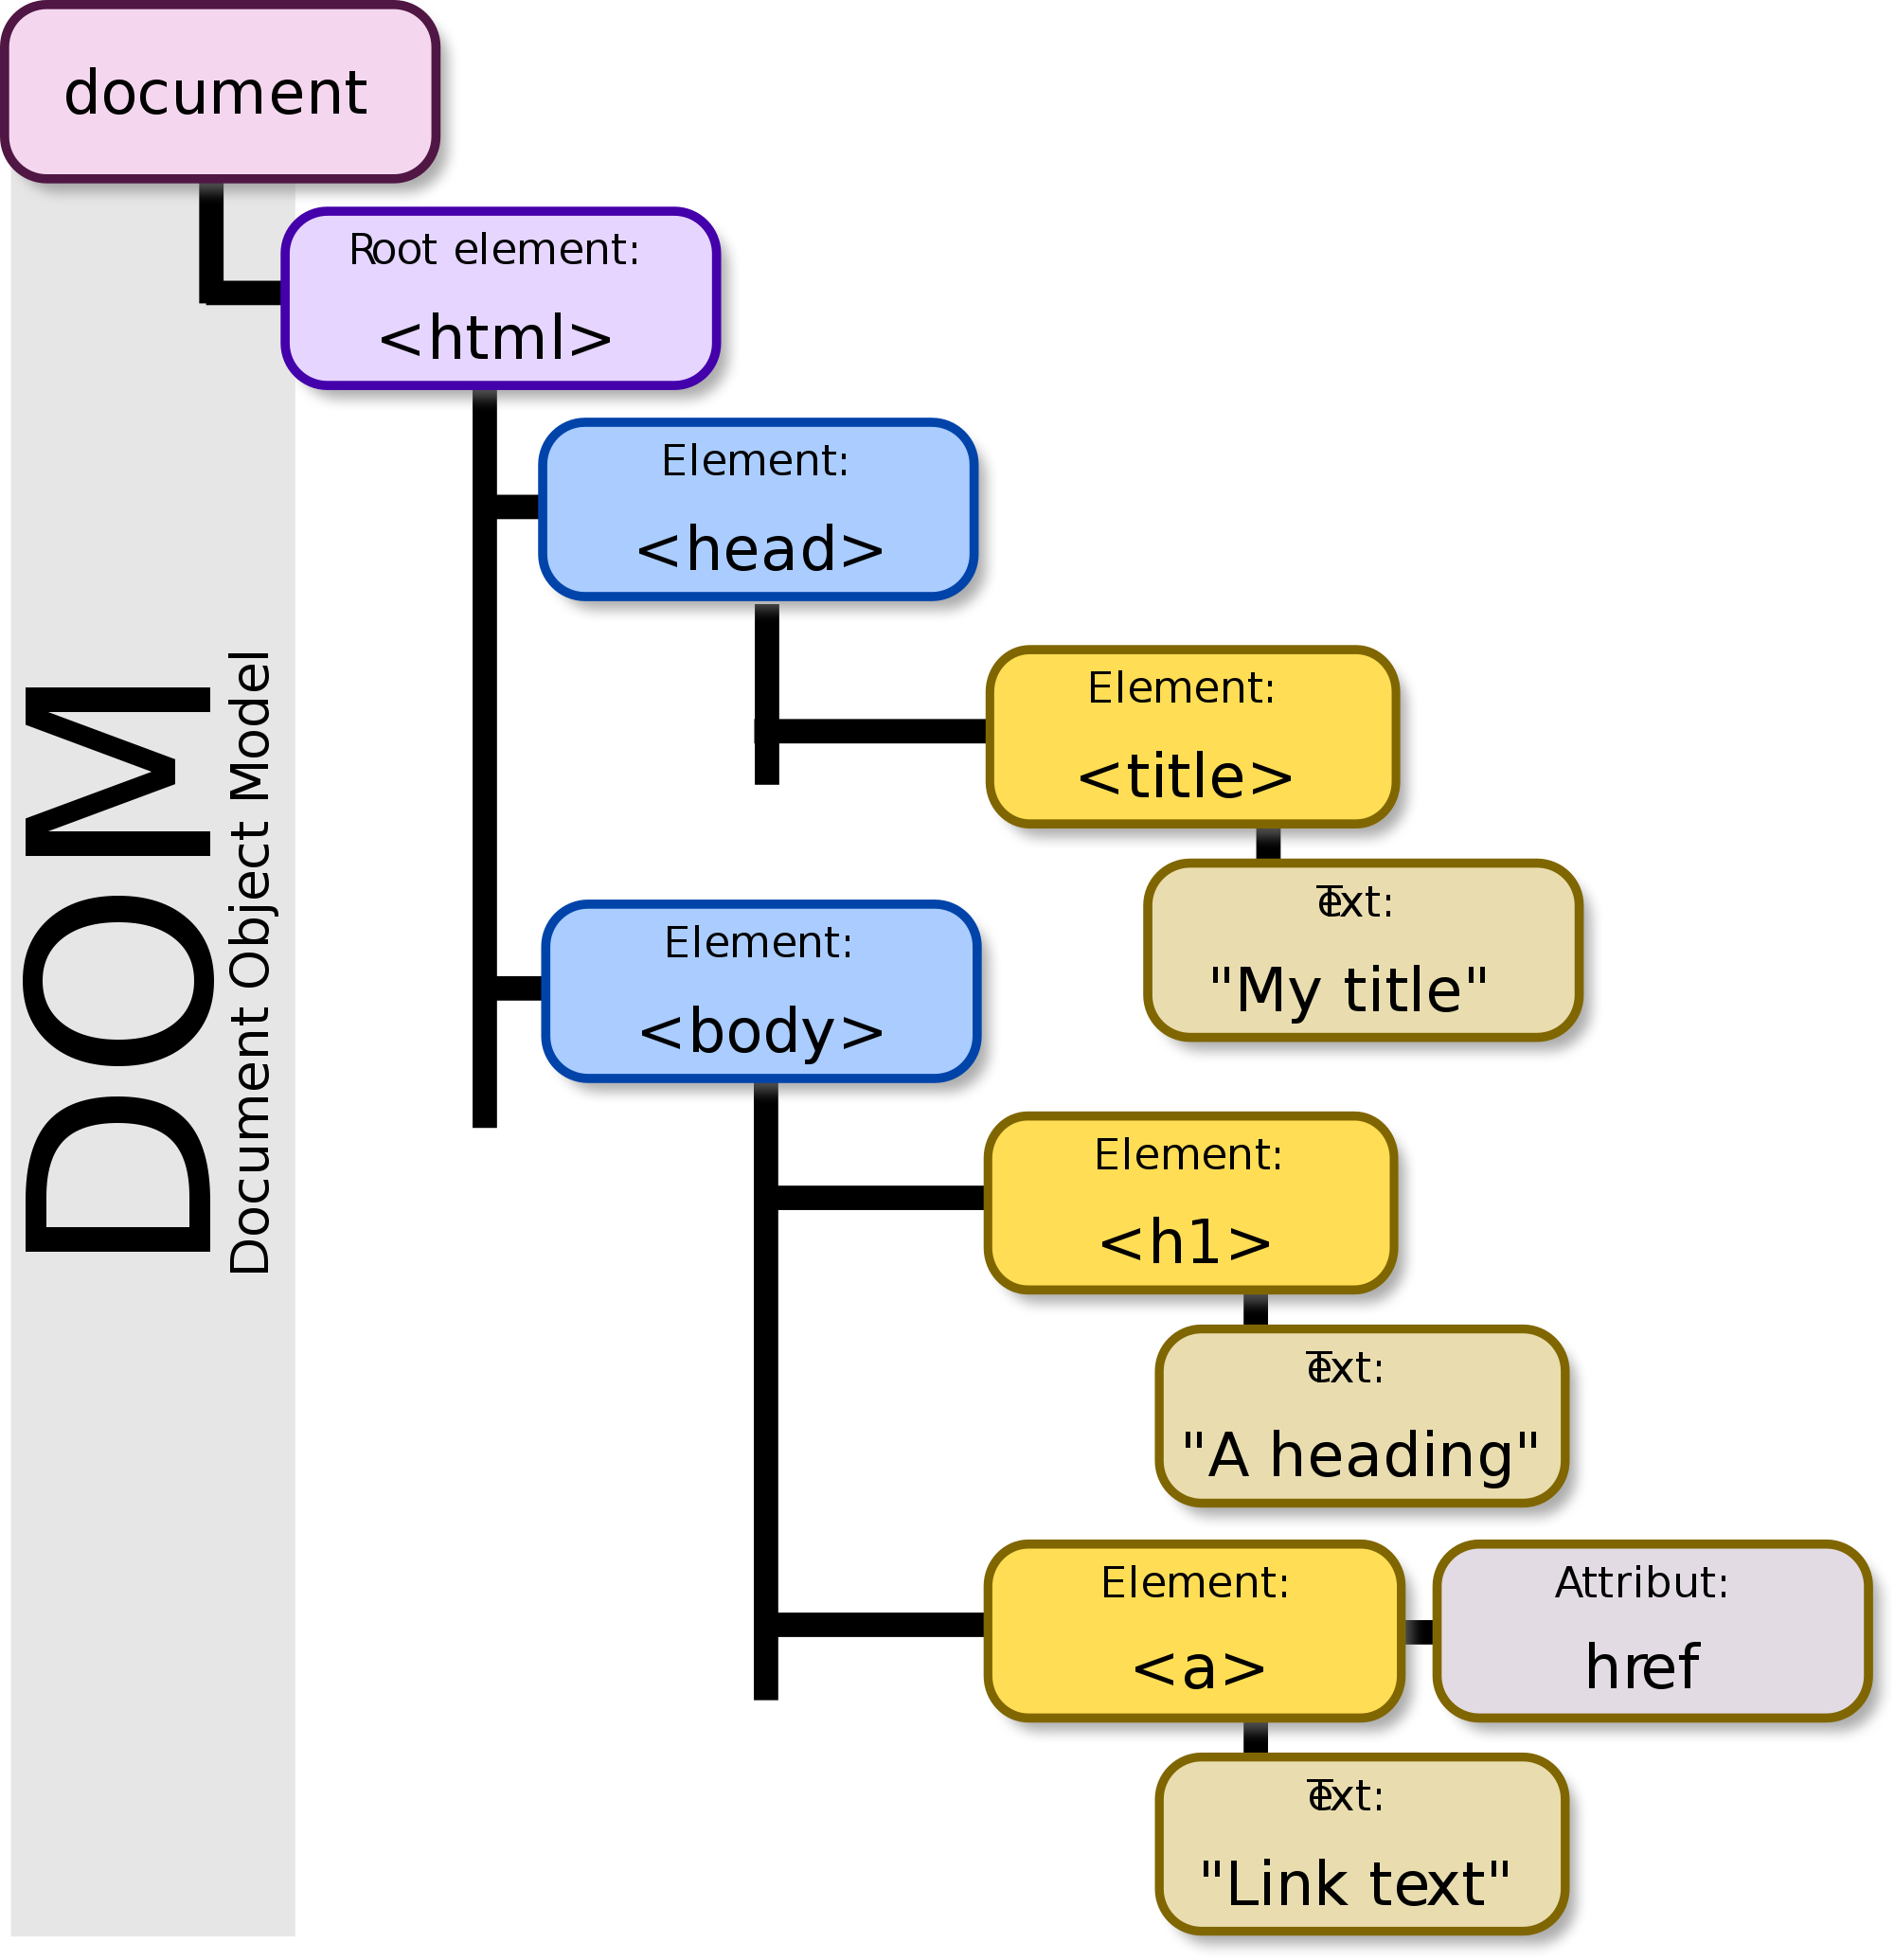
\includegraphics[width=0.75\linewidth]{./3_Tecnologias/Img/DOMModel.png}
\end{center}
\caption{Esquema general del DOM.}
\source{https://en.wikipedia.org/wiki/Document\_Object\_Model}
\label{DOMModel}
\end{figure}


Aunque en este TFG se trabaja con el estándar de JavaScript llamado ECMAScript 2016, en la actualidad la última versión es ECMAScript 2017, lanzada en Junio de este mismo año. A continuación se detallan algunos elementos de importancia que se utilizaron en la elaboración de este TFG. Su lugar de uso se detalla en el siguiente capítulo del presente documento.

\paragraph{\emph{Web Real-Time Communications}} ~\\

WebRTC es una tecnología que permite a las aplicaciones Web capturar y transmitir datos de audio y vídeo, así como intercambiar datos entre navegadores sin un intermediario. Los estándares que componen WebRTC hacen posible compartir datos y realizar videoconferencias \emph{peer-to-peer}, sin que sea necesario que los usuarios instalen complementos u otros elementos \emph{software} de terceros. Junto a las API \emph{MediaStream Recording} y \emph{Media Capture and Streams} proporcionan a la Web una gama de capacidades multimedia que incluyen captura y grabación de multimedia en disco, conferencias de audio y vídeo, intercambio de archivos e incluso gestión de identidad.

Es un estándar actualmente en desarrollo por la \emph{World Wide Web Consortium} (\acrshort{W3C}) y el IETF. Para transferir los datos multimedia se utiliza el protocolo \emph{Realtime Transport Protocol }(\acrshort{RTP}).

El \emph{getUserMedia()} es el método principal mediante el que se solicitan al usuario los permisos necesarios para usar un dispositivo de entrada multimedia (como la cámara o el micrófono). Produce una interfaz \emph{MediaStream} consistente en las pistas de los tipos de multimedia solicitados. Generalmente se usa accediendo a la interfaz \emph{MediaDevices} con la siguiente orden \mintinline[breaklines=true, breakbytokenanywhere=true]{javascript}{navigator.mediaDevices.getUserMedia(constraints).then(...)} siendo \emph{constraints} el parámetro que indica el tipo de multimedia que se solicita y then la función que contendría los callbacks a ejecutar en caso de éxito o error según la \emph{Promise API}.

La API \emph{MediaStream Recording} está muy relacionada captura los datos generados por el objeto \emph{MediaStream} para su análisis, procesado o guardado en disco. Se basa en una única interfaz, \emph{MediaRecorder}, que se encarga de obtener los datos del \emph{MediaStream} mediante una serie de eventos. El proceso de grabación es muy sencillo:

\begin{itemize}
\item Se crea el \emph{MediaStream} fuente de los datos multimedia.
\item Se crea el objeto \emph{MediaRecorder}, especificando la transmisión de origen y otras opciones pertinentes.
\item Configurar el gestor \emph{MediaRecorder.ondataavailable} para el evento \emph{dataavailable}, que sería llamado cada vez que haya datos disponibles.
\item Controlar el proceso de grabación mediante los métodos disponibles, por ejemplo con \emph{MediaRecorder.start()} para comenzar y \emph{MediaRecorder.stop()} para detener la grabación.
\item El evento \emph{dataavailable} tiene un atributo \emph{data} que contiene la información multimedia adquirida, pudiendo procesarse como se requiera.
\end{itemize}

La transmisión de datos en Web puede verse enormemente beneficiada por JSON soportado de forma nativa desde ECMAScript 5, aunque debido a su popularidad son ya muchos los lenguajes que han incluido generadores y analizadores de su sintaxis.

\paragraph{\emph{AJAX}} ~\\

El AJAX utiliza peticiones HTTP para que las aplicaciones Web puedan enviar datos al servidor y recibir datos del mismo en segundo plano, sin interferir en el comportamiento y la visualización de la Web. De este modo, junto a la manipulación del DOM realizada por JavaScript, se permite cambiar el contenido dinámicamente con información procedente del servidor sin tener que actualizar la totalidad de la página. En la actualidad se utiliza JSON en lugar de XML por su integración nativa con JavaScript.

\paragraph{\emph{jQuery}} ~\\

A menudo, trabajar con determinadas funciones de JavaScript (manipulación del DOM, manejar eventos, usar AJAX) puede generar documentos difíciles de leer por su extensión y lo confuso de su sintaxis. La jQuery es una biblioteca JavaScript gratuita y de código abierto que trata de simplificar todos estos procesos del lado del cliente. Permite a los desarrolladores crear complementos con los que añadir una capa más de abstracción a las interacciones de bajo nivel siguiendo un enfoque modular. Actualmente se halla en su versión 3. Para utilizarlo en un sitio Web ha de ser incluido como se incluiría un archivo JavaScript cualquiera en un archivo HTML. La popularidad de jQuery radica en cómo simplifica la lectura y el análisis del código. Por ejemplo, si desde un archivo JavaScript deseamos realizar una petición AJAX de tipo GET al archivo del servidor \emph{send-ajax.php} se tendría que escribir el bloque de código \ref{AJAX} (cliente).

\begin{listing}[H]
\begin{minted}
[
frame=lines,
framesep=2mm,
baselinestretch=1.2,
bgcolor=lightgray,
fontsize=\footnotesize,
breaklines=true,
breaksymbolleft={}
]
{javascript}
// Inicializar la petición HTTP.
var xhr = new XMLHttpRequest();
xhr.open('get', 'send-ajax-data.php');

// Monitorizar los cambios de estado de la petición.
xhr.onreadystatechange = function () {
    var DONE = 4; // readyState = DONE significa que la petición se ha hecho.
    var OK = 200; // status 200 es un retorno con éxito.
    if (xhr.readyState === DONE) {
        if (xhr.status === OK) {
            console.log(xhr.responseText); // Aquí estaría la respuesta del servidor
        } else {
          console.log('Error: ' + xhr.status); // Ha ocurrido un error durante la petición.
        }
    }
};
// Enviar la petición a send-ajax-data.php
xhr.send(null);
\end{minted}
\caption{Petición AJAX normal}
\label{AJAX}
\end{listing}

El mismo ejemplo utilizando jQuery, donde el carácter \$ representa el objeto jQuery a través del cual se accede a todos sus usos, se muestra en el bloque de código \ref{jQueryAJAX}.

\begin{listing}[H]
\begin{minted}
[
frame=lines,
framesep=2mm,
baselinestretch=1.2,
bgcolor=lightgray,
fontsize=\footnotesize,
breaklines=true,
breaksymbolleft={}
]
{javascript}
$.get('send-ajax-data.php')
    .done(function(data) {
        console.log(data);
    })
    .fail(function(data) {
        console.log('Error: ' + data);
    });
\end{minted}
\caption{Petición AJAX con jQuery}
\label{jQueryAJAX}
\end{listing}

\paragraph{\emph{Bootstrap}} ~\\

Bootstrap es un \emph{framework} que simplifica la carga de trabajo, adaptada para el diseño de aplicaciones móviles. Contiene plantillas basadas en HTML y CSS para tipografías, formas, botones, navegación y otros componentes, así como algunos componentes opcionales de JavaScript. Utiliza un sistema de rejilla o \emph{grid} para ayudar en el diseño de la web, proporcionando así un sencillo sistema de filas, cada una de ellas subdividida hasta en 12 columnas, con el que puede establecerse la proporción visual de los elementos de la pantalla. En la Figura \ref{gridBootstrap} se muestra un ejemplo de uso del sistema de rejilla en Bootstrap, con un elemento sirviendo de cabecera y varios contenedores alineados bajo el mismo en grupos de tres.

\begin{figure}[!t]
\begin{center}
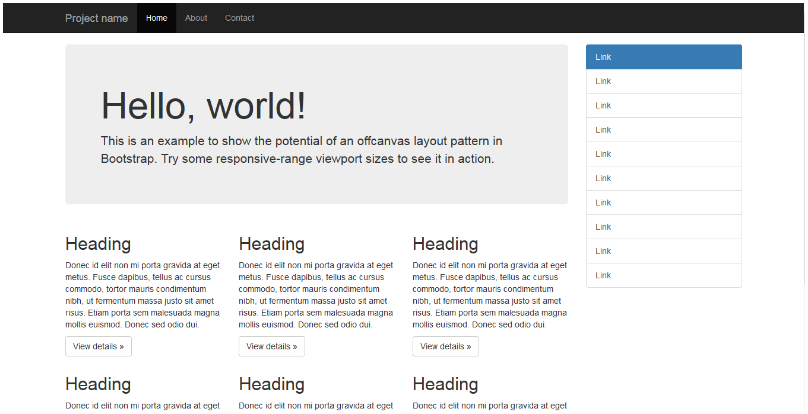
\includegraphics[width=0.75\linewidth]{./3_Tecnologias/Img/gridBootstrap.png}
\end{center}
\caption{Ejemplo de diseño con Bootstrap.}
\source{http://getbootstrap.com/docs/4.0/examples/offcanvas/}
\label{gridBootstrap}
\end{figure}
\cleardoublepage
\clearpage
\vspace*{\stretch{2}}%{\fill}
\begin{center}
\begin{minipage}{.75\textwidth}
\section{Análisis previo y funcional}

Una vez revisada la idea general que se busca en este TFG y las tecnologías de las que hacemos uso para lograrlo, en este capítulo mostramos el análisis previo (requisitos) y el funcional (visión de alto nivel de los distintos módulos funcionales principales de que consta el sistema). % \pagebreak
\end{minipage}
\end{center}
\vspace{\stretch{3}} % \vfill % equivalent to \vspace{\fill}
\clearpage% https://tex.stackexchange.com/questions/70714/center-horizontally-and-vertically-a-block-of-text

\subsection{Objetivo y análisis de requisitos}
El objetivo de nuestro sistema de sensado móvil colaborativo, asimétrico con beneficio para todos los participantes, es implantar un sistema capaz de ofrecer un servicio de conexión WiFi a Internet a cambio de datos procedentes del sensor de audio (micrófono) del dispositivo móvil que utilice el cliente (aunque no limitado a este tipo de dispositivos). Para ello utilizamos una combinación de hardware y aplicaciones software ya existente, programando desde cero los módulos restantes.

Los requisitos del sistema son los siguientes:

\begin{itemize}
\item Soporte para múltiples navegadores y sistemas operativos, incluyendo móviles.
\item Mínima interacción con el usuario: sólo se requiere de la provisión de permisos la primera vez que se utiliza el sistema en un Punto de acceso determinado. Si se cambia de punto de acceso es necesario volver a dar permisos.
\item Que proporcione más datos aparte de los del sensor de audio.
\item Proveer distintos modos de conexión a Internet.
\end{itemize}

El primer requisito podría alcanzarse de forma sencilla. Dado que a priori vamos a emplear tecnología Web basándonos en estándares que todos los navegadores modernos deben estar preparados para procesar no se requeriría instalar ninguna aplicación o complemento de navegador adicional en los clientes del servicio. Además, se tendría en cuenta el diseño Web responsivo, de forma que la visualización del contenido se adapte al tamaño y características del dispositivo. Sin embargo, existen ciertas particularidades.

Los estándares utilizados para implantar la funcionalidad de captura de sonido, como WebRTC y MediaStream Recording, están aún abiertos y tienen poco tiempo, por lo que solo están soportados en versiones muy recientes de los navegadores o incluso, hasta hace poco tiempo, únicamente en sus versiones experimentales. Por ejemplo, Safari, el navegador Web de Apple por defecto para sus ordenadores con MacOS y los dispositivos iOS, ha comenzado a trabajar con los estándares WebRTC y relacionados hace tan solo un año, anunciando su compatibilidad para la versión 11 del navegador que salida en Septiembre de 2017. Por el momento, para Safari solo puede encontrarse una compatibilidad preliminar en su versión para desarrolladores, Safari Technology Preview \cite{SafariWebRTC}.

En cuanto al segundo requisito, se plantea que las únicas interacciones que tenga que hacer el usuario con el servicio intermedio de portal cautivo antes de obtener acceso a Internet sea la concesión de permisos de ubicación y captura de audio y otro botón para comenzar el proceso de conexión, representando una ventaja sobre otros sistemas de portal cautivo donde hay múltiples redirecciones, procesos de creación de cuentas de usuario y de inicio de sesión.

Para alcanzar el tercer requisito se trata de aumentar la usabilidad del servicio más allá de capturar un fragmento de sonido, obteniendo también su ubicación y una marca de tiempo para poder hacer análisis estadísticos, mapeos de niveles de señal 3D en función del tiempo, etc.

El cuarto requisito ha surgido a partir de las pruebas realizadas y el desarrollo iterativo e incremental del sistema. Esto es, inicialmente se especificó únicamente un modo de conexión a Internet debiendo el cliente Web mantener abierta la pestaña del navegador Web en la que se proporcionó el permiso para acceder al micrófono. La aplicación javascript de esa pestaña capturaba un fragmento de audio de 5 segundos cada 3 minutos. La ventaja es que la ofrece al usuario una conexión más estable. La desventaja es que retiene el control del micrófono en modo exclusivo para esa aplicación Javascript. Haciendo desarrollos incrementales se detectó este comportamiento a priori no explícito, por lo que se observó que este comportamiento no sería adecuado para aquellos usuarios que quisieran hacer uso del micrófono a la vez que está conectado a Internet (por ejemplo, mensajería de audio vía aplicaciones de mensajería instantánea). Por ello, en segundo lugar se especificó como requisito previo que pudiera existir un nuevo modo de conexión a Internet. Esto es, ofrecer un tiempo de conexión fijo de 30 minutos a cambio de un único archivo de audio inicial, tras lo cual podría cerrarse la pestaña del navegador de la Aplicación Web y hacer uso libre del micrófono del dispositivo durante este tiempo.

\subsection{Análisis previo}

El sistema está compuesto de varios elementos que interactúan entre sí. A continuación se ofrece un resumen del funcionamiento de cada elemento, los módulos que lo componen y las tareas asociadas a los mismos:

\begin{itemize}
\item \emph{Hardware necesario}: se supone que en el local a monitorizar ya existe un acceso a Internet al cual se puede conectar un Punto de acceso WiFi. Por ello, únicamente es necesario una Raspberry Pi 3 Model B con el sistema operativo Raspbian, un módulo software controlador del módulo WiFi 802.11 (Hostapd) para habilitar su funcionamiento como Punto de Acceso, el software de control de acceso y el servicio de portal cautivo. La configuración de este software para que funcionara adecuadamente llevó mucho tiempo debido a la falta de información o bien información obsoleta sobre estas aplicaciones. Por ello hubo de realizarse muchas pruebas de ensayo-error hasta que definitivamente pudimos dar con la configuración correcta.
\item \emph{Aplicaciones software configurables}: para proveer el acceso a Internet es necesario utilizar las siguientes aplicaciones que ya existen y que se deben configurar adecuadamente. Destacar que esta tarea de configuración no es sencilla, debido a la falta de información veraz, la obsolescencia de la información existente y la dificultad de instalarlos en la Raspberry Pi 3. Por este motivo hubo de realizar múltiples pruebas de ensayo y error hasta dar con la configuración adecuada, cuyas ideas generales proporcionamos a continuación:
\begin{itemize}
\item \emph{Control de acceso}:
\begin{itemize}
\item \emph{RADIUS}: necesario para la autenticación de los usuarios. Se utilizó el daloRADIUS, para la gestión interna del acceso de usuarios, recibiendo las credenciales proporcionadas por el servicio de portal cautivo y gestionando su conexión.
\item \emph{CovaChilli y su entorno}: necesario para redirigir correctamente los paquetes entrantes (autorizados previamente por RADIUS) desde la interfaz inalámbrica a la interfaz cableada y viceversa. Aquí hubo que configurar las ubicaciones de nuestro portal cautivo propio, los ajustes de autenticación de usuarios y habilitar el uso de \acrshort{SSL}.
\end{itemize}
\item \emph{Node.js}: necesario para implementar el servidor donde alojar nuestro portal cautivo, recibir y procesar los ficheros de audio generados e instalar servicios de monitorización del mismo.
\end{itemize}
\item \emph{Aplicaciones software desarrolladas desde cero}:
\begin{itemize}
\item \emph{Portal cautivo}: enlaza a los usuarios con el control de acceso mediante un sistema de control de usuarios intermedio, realizando también la tarea de captura y almacenamiento de archivos de audio procedentes de los micrófonos de los dispositivos, que es lo que da sentido al sistema global. Su funcionalidad se detalla a continuación. Su funcionalidad básica es:
\begin{itemize}
\item \emph{Servidor Web}: implantado con Node.js, se encargaría de lo siguiente:
\begin{itemize}
\item Servir la aplicación Web a los usuarios que se conecten a la red.
\item Recibir y almacenar archivos de audio de los usuarios conectados.
\item Llevar un control de los usuarios a los que se ha dado acceso a Internet.
\item Informar a los clientes del estado del servidor.
\end{itemize}
\item \emph{Cliente Web}: implantado con , HTML, CSS y JavaScript, y se encarga de lo siguiente:
\begin{itemize}
\item Ser el punto de entrada de los usuarios al sistema, ofreciendo dos modalidades de conexión diferentes.
\item Comprobar el estado del servidor.
\item Adquirir datos de ubicación y marca de tiempo de los usuarios.
\item Capturar una señal de audio de los usuarios en intervalos constantes.
\item Enviar la señal de audio al servidor.
\item Pedir credenciales de usuario al servidor.
\item Conectar al usuario a Internet con las credenciales recibidas. 
\end{itemize}
\end{itemize}
\end{itemize}
\end{itemize}

\subsection{Análisis funcional}

La estructura global del sistema podría entenderse como un conjunto de módulos que proporcionen un nivel de abstracción adicional, útil para comprender el sistema. Después, pueden dividirse estos módulos en otros submódulos que representen las funciones desempeñadas por cada uno de ellos individualmente en el sistema global. Muchos de estos submódulos representan instalaciones de \emph{software} completas en sí mismas.

Considerando esta aproximación al sistema podemos representar el mismo como una combinación de tres módulos o capas, todos ellos implantados sobre el \emph{hardware} anteriormente mencionado y interrelacionados entre sí. En la Figura \ref{modulos} se muestra el conjunto de módulos principales considerados.

\begin{figure}[!t]
\begin{center}
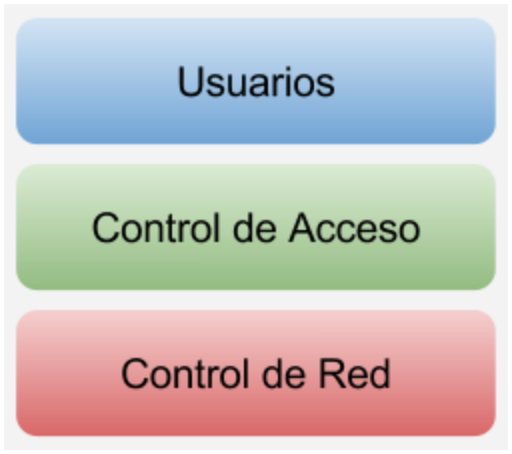
\includegraphics[width=0.5\linewidth]{./4_AnalisisFuncional/Img/modulos.png}
\end{center}
\caption{Diagrama de módulos funcionales}
%\source{http://coova.github.io/CoovaChilli/}
\label{modulos}
\end{figure}

Un primer módulo de \emph{Usuarios} consiste tanto en la única interfaz que los usuarios del sistema (\emph{Vista}) como el servidor que proporciona dicha interfaz junto a un primer control de usuarios (\emph{Controlador} y una parte del \emph{Modelo} relacionado con las acciones que lleva a cabo el servidor). El segundo módulo es el de \emph{Control de Acceso}, que incluye todo el software dedicado a esta gestión, formado por CoovaChilli y su entorno (\emph{Observador}). Por último se halla el módulo de Control de Red, que incluye todo el \emph{software} que permite a la Raspberry Pi funcionar como Punto de Acceso inalámbrico y la configuración de las diferentes redes que entran en juego en el sistema.

Huelga decir que, si bien los clientes del servicio solo interactuarían con el módulo de Usuarios, los otros dos módulos del sistema son accesibles a un administrador, que se encargaría de su correcta configuración inicial y posterior mantenimiento.

\subsubsection{Módulo Usuarios}
Es el módulo de más alto nivel y el único punto de contacto visible de los usuarios con el servicio. Está compuesto de cinco submódulos; un grupo de tres submódulos que interactúan entre sí para proporcionar el servicio, que son la aplicación Web, el servidor y el control de usuarios; un módulo que hace de interfaz con el módulo inferior de Control de Acceso, biblioteca CoovaChilli; y un último módulo que configura y controla el uso de esta interfaz. En la Figura \ref{moduloUsers} se muestra un esquema básico de las relaciones entre los diferentes submódulos que conforman la capa de Usuarios.

\begin{figure}[!t]
\begin{center}
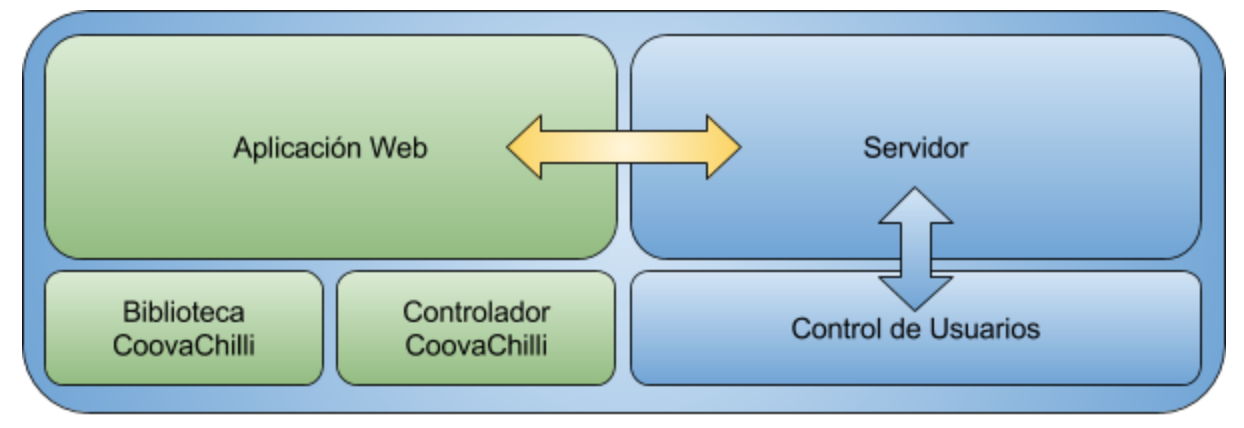
\includegraphics[width=0.75\linewidth]{./4_AnalisisFuncional/Img/moduloUsers.png}
\end{center}
\caption{Diagrama de submódulos del módulo Usuarios}
%\source{http://coova.github.io/CoovaChilli/}
\label{moduloUsers}
\end{figure}

La \emph{Aplicación Web} contiene los datos del portal cautivo al que se redirigen los clientes cuando traten de conectarse a la red inalámbrica. Sus funciones, ya adelantadas en el análisis previo pero ampliadas aquí, son:

\begin{itemize}
\item Adquirir los permisos de ubicación y captura de audio del usuario.
\item Comprobar el estado del servidor para evitar hacer el proceso si este está lleno (haciendo imposible la conexión al servicio).
\item Capturar una muestra corta de dicho audio una única vez o a intervalos regulares, dependiendo del modo de conexión escogido, y enviarla al servidor.
\item Recibir las credenciales de usuario enviadas por el servidor, utilizando como nombre de archivo las coordenadas y la marca de tiempo de la última consulta de geolocalización.
\item Gestionar la conexión de los usuarios con las credenciales recibidas, todo ello por medio de la configuración y las funciones de la biblioteca CoovaChilli y su controlador.
\item Además, está programada para cerrar la conexión si su pestaña del navegador se cierra o se recarga de alguna forma.
\end{itemize}

En la Figura \ref{flujoSistema} se muestra un diagrama de flujo con la funcionalidad básica del sistema en una primera conexión. En este diagrama se omite la fase de elección de los diferentes modos de conexión.

\begin{figure}[!t]
\begin{center}
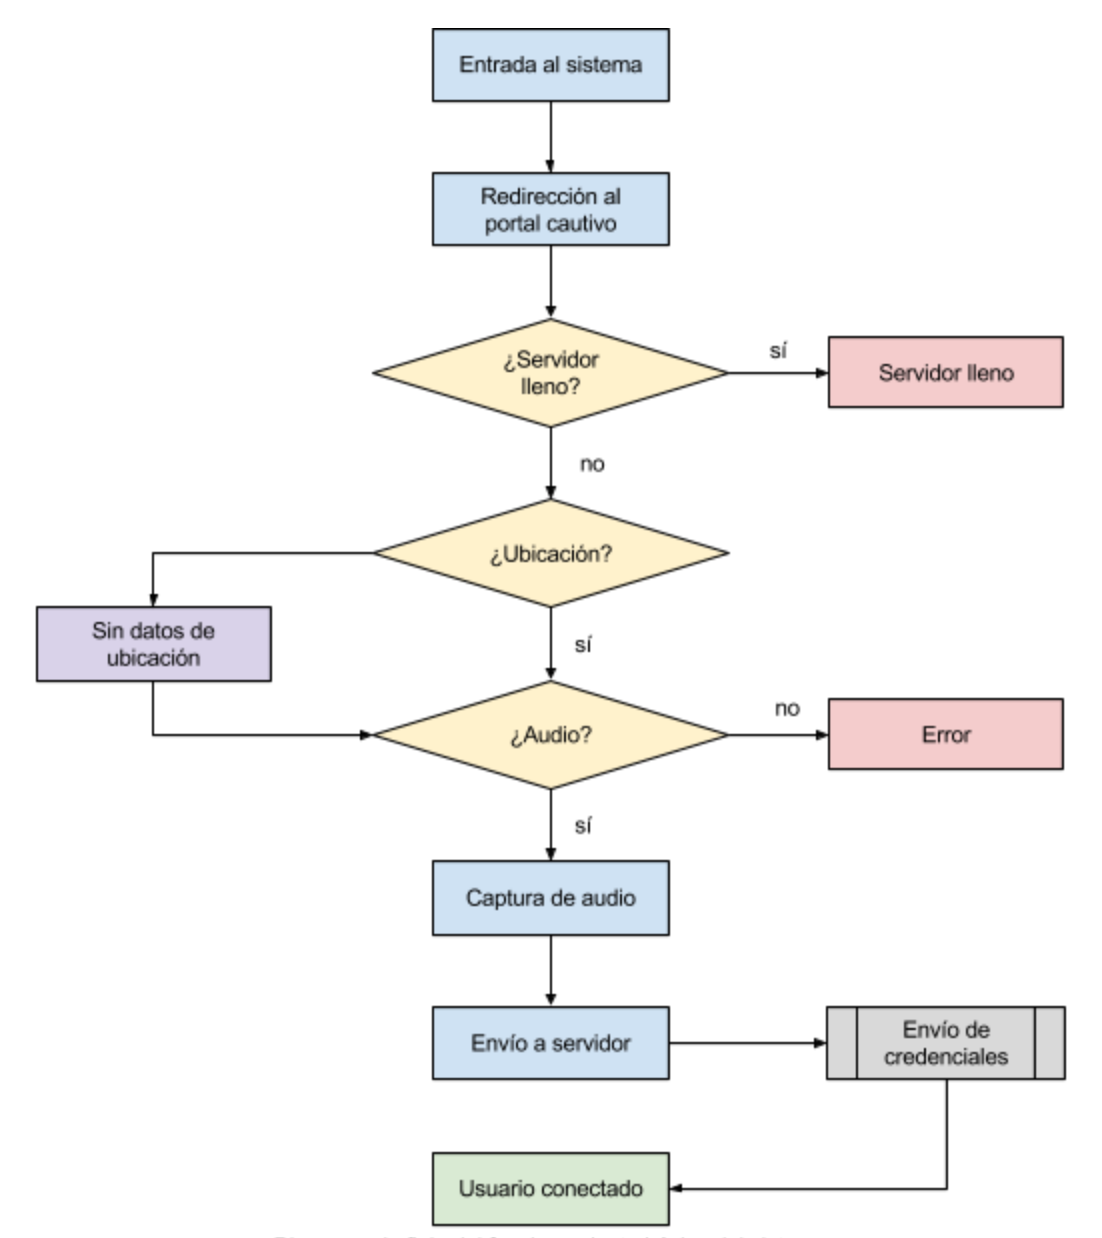
\includegraphics[width=0.75\linewidth]{./4_AnalisisFuncional/Img/flujoSistema.png}
\end{center}
\caption{Diagrama de la funcionalidad de la conexión a Internet a través del portal cautivo modificado}
%\source{http://coova.github.io/CoovaChilli/}
\label{flujoSistema}
\end{figure}

Todas las consultas que ocurren entre la aplicación Web y el servidor utilizan peticiones GET y POST gestionadas mediante AJAX.

El \emph{Servidor} se encarga de enviar la Aplicación Web en forma de HTML estático a los usuarios que realicen peticiones al mismo, y de comunicarse con los clientes y el Control de Usuarios para aportar la funcionalidad deseada. Sus funciones ampliadas son:

\begin{itemize}
\item Servir la Aplicación Web.
\item Comprobar el estado del servidor comunicándose con el \emph{Control de Usuarios}, informando a la \emph{Aplicación Web} si el servicio está disponible o por el contrario está lleno, con lo que no podría prestarse el servicio.
\item Si recibe un archivo de audio de un cliente que aún no tiene credenciales asignadas, pide al \emph{Control de Usuarios} unas credenciales que se encuentren disponibles en su base de datos y las almacena a la espera de que la \emph{Aplicación Web} las pida.
\item Enviar las credenciales almacenadas a la \emph{Aplicación Web}, informando al \emph{Control de Usuarios} para que marque dichas credenciales como utilizadas.
\item Recibir notificaciones de desconexión de usuarios por parte de la \emph{Aplicación Web} y pasar dicha información al \emph{Control de Usuarios} para marcar un usuario como libre en la base de datos.
\end{itemize}

Para llevar a cabo todas estas tareas se utiliza Node.js, los módulos de npm \emph{Express} para la funcionalidad de servidor, \emph{Formidable} para la gestión de archivos de audio entrantes. \emph{Body-Parser} para leer determinadas variables procedentes de la Aplicación Web y los módulos del núcleo de Node.js, Fs para acceder al sistema de archivos y escribir en él y Path para trabajar con las rutas de archivos y directorios.

El \emph{Control de Usuarios} se encarga de gestionar los usuarios activos e inactivos por medio de una base de datos sencilla, implementada con dos archivos JSON, uno para cada modo de conexión, y dos archivos JavaScript que controlan a cada archivo JSON por separado actuando como módulos Node.js del \emph{Servidor}. Si la cantidad de usuarios posible se hiciera lo suficientemente grande, este módulo y su archivo JSON podrían ser reemplazados por una aplicación de base de datos más potente (MySQL, MongoDB...). Los archivos base de datos JSON constan de un \emph{array} de usuarios, cada uno de ellos con los siguientes atributos:

\begin{itemize}
\item \emph{id}: un número entero igual o superior a 0 que actúa como identificador interno de usuario.
\item \emph{username}: el nombre del usuario.
\item \emph{password}: la contraseña del usuario.
\item \emph{isActive}: una variable booleana, que tiene la asignación \emph{true} si el usuario está ocupado y \emph{false} en caso contrario.
\end{itemize}

Las funciones de los archivos JavaScript que controlan al archivo JSON anterior son:

\begin{itemize}
\item Buscar un usuario inactivo en el archivo de base de datos, devolviendo el identificador y las credenciales de dicho usuario si lo hubiera.
\item Asignar usuarios como activos o inactivos escribiendo en el atributo \emph{isActive} correspondiente.
\item Hacer externas las credenciales del usuario seleccionado para que el \emph{Servidor} pueda accederlas y hacer sus operaciones.
\end{itemize}

La biblioteca \emph{CoovaChilli} es un archivo JavaScript denominado \verb+ChilliController.js+, proporcionado por la instalación de CoovaChilli en el directorio \verb+/etc/chilli/www/+. Se encarga de enlazar la Aplicación Web con la interfaz JSON de CoovaChilli creando el objeto global \emph{chilliController}, que puede utilizar los métodos descritos en el capítulo anterior para gestionar la conexión y desconexión de usuarios al servicio.

Por último, el \emph{Controlador CoovaChilli} es un archivo JavaScript de configuración, que modifica los atributos por defecto del objeto \emph{chilliController} creado por la biblioteca CoovaChilli y enlaza los métodos de dicho objeto con acciones concretas de la Aplicación Web.

\subsubsection{Módulo Control de Acceso}
Este módulo está basado en instalaciones y configuraciones de \emph{software} concernientes la gestión interna del control de acceso al servicio. Puede dividirse en tres submódulos: \emph{CovaChilli}, \emph{Servidor RADIUS} e \emph{Interfaz Web de control de RADIUS}. Hemos preferido denominar a los dos primeros submódulos con los nombres originales del software utilizado por claridad. La funcionalidad que aprovechamos de estas aplicaciones es la que tienen, en particular, para este TFG. La tarea aquí básicamente es encontrar, tarea no sencilla, la instalación y configuración adecuada de estos submódulos. El tercer submódulo es una implantación propia que llevó mucha dificultad debido a la complejidad de la conexión entre estos submódulos. En la Figura \ref{moduloControlAcceso} se muestra un diagrama de estos submódulos.

\emph{CoovaChilli} es el submódulo que se encarga de la mayor parte del trabajo. Redirige las conexiones entrantes no autenticadas al portal cautivo implantado en el módulo de \emph{Usuarios} y mantiene un contacto constante con el \emph{Servidor RADIUS}. Como parte de este submódulo se destaca también la \emph{Interfaz JSON}, que viene incluida en la instalación de CoovaChilli y hace posible comunicar dicho \emph{software} con nuestra \emph{Aplicación Web}.

El \emph{Servidor RADIUS} es el gestor de AAA requerido por CoovaChilli para funcionar, aunque es posible implantar otro tipo de servicios para llevar a cabo esta gestión, en este TFG se ha utilizado la aplicación \emph{FreeRADIUS}. En este submódulo también se incluye todo aquel \emph{software} que sea obligatorio para que el servidor funcione, como las instalaciones de bases de datos y su respectiva configuración.

Por supuesto, para que el sistema pueda funcionar, la base de usuarios del \emph{servidor RADIUS} y la existente en los archivos JSON del submódulo \emph{Controlador de Usuarios}, pertenecientes al módulo de de \emph{Usuarios}, ha de ser la misma.

Opcionalmente, puede instalarse un administrador gráfico del Servidor RADIUS para hacer más intuitiva su gestión. En este caso se incluye el submódulo \emph{Interfaz Web de control RADIUS}, representada por una instalación del administrador Web daloRADIUS funcionando sobre el servidor Web \emph{NGINX}.

\begin{figure}[!t]
\begin{center}
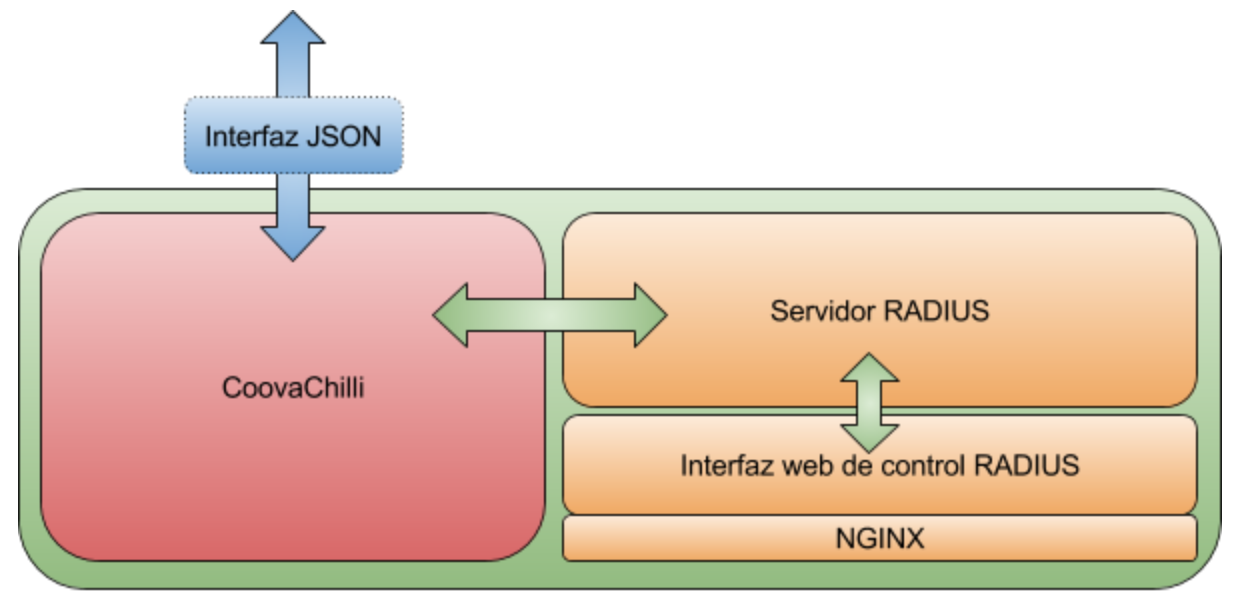
\includegraphics[width=0.75\linewidth]{./4_AnalisisFuncional/Img/moduloControlAcceso.png}
\end{center}
\caption{Diagrama de submódulos del módulo Control de Acceso}
%\source{http://coova.github.io/CoovaChilli/}
\label{moduloControlAcceso}
\end{figure}

\subsubsection{Módulo Control de Red}
El módulo de \emph{Control de Red} es el de más bajo nivel de nuestro sistema, encargado de configurar y gestionar el comportamiento de los componentes \emph{hardware} de la Raspberry Pi. Puede dividirse en tres submódulos: la \emph{Configuración de las Interfaces de Red}, \emph{Hostapd} y el propio dispositivo sobre el que opera todo el servicio: la \emph{Raspberry Pi} con el sistema operativo Raspbian. Hemos preferido denominar a los módulos segundo y tercero como la aplicación original y el hardware por simplicidad para que se entienda que en esos módulos la tarea principal fue la de instalarlos y configurarlos adecuadamente (recurriendo a la técnica de ensayo y error en la mayoría de la veces). En la Figura \ref{moduloControlRed} se muestra el esquema de submódulos de este módulo. 

\begin{figure}[!t]
\begin{center}
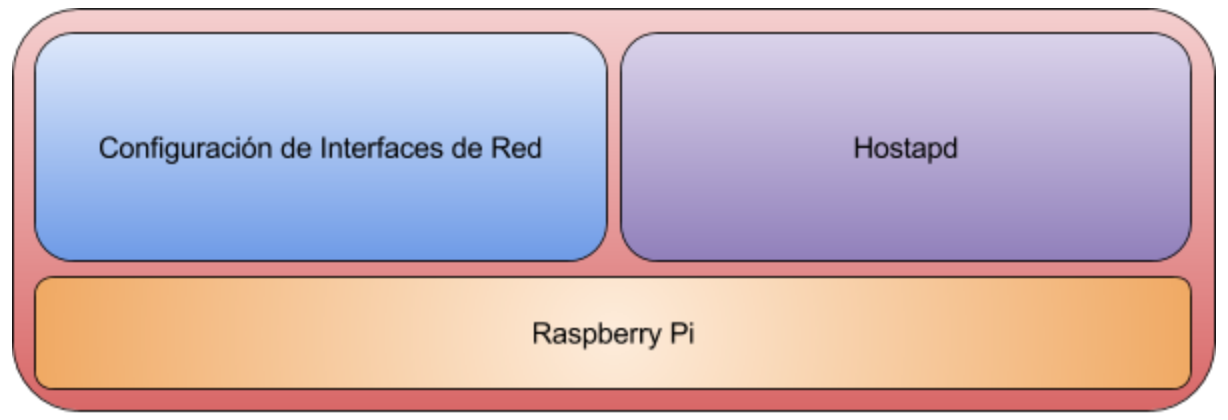
\includegraphics[width=0.75\linewidth]{./4_AnalisisFuncional/Img/moduloControlRed.png}
\end{center}
\caption{Diagrama de submódulos del módulo de Control de Red}
%\source{http://coova.github.io/CoovaChilli/}
\label{moduloControlRed}
\end{figure}

El submódulo \emph{Configuración de Interfaces de Red} consiste en utilizar las herramientas instaladas en Raspbian (adquiriendo las que no estén disponibles por defecto) para implantar y configurar las redes necesarias para el funcionamiento del sistema. Las dos redes principales que intervienen, la cableada Ethernet \emph{eth0} y la inalámbrica \emph{wlan0}, varían su configuración según el entorno en el que se encuentren. La \emph{wlan0} debe configurarse con IP estática y se le debe asignar la red correspondiente, dado que va a ser nuestro Punto de Acceso WiFi.

La configuración de \emph{eth0} depende de la red que proporciona el acceso a Internet al sistema. Por ejemplo, la red cableada de la Universidad (donde hicimos pruebas) solo es accesible cuando la interfaz tiene una IP determinada en el punto de conexión, no pudiendo conectarse si no se asigna la IP adecuada. En una instalación de Internet casera puede configurarse la interfaz sin IP y dejar que el DHCP del router de la instalación asigne una dirección adecuada para establecer su red local.

Esta configuración incluye el paso necesario de habilitar el \emph{flag} del \emph{kernel} Linux del sistema operativo Raspbian para que permita el proceso de reenvío de paquetes IP, o IP forwarding, desde la interfaz cableada a la inalámbrica y viceversa. Sin este paso la instalación de CoovaChilli, que basa su funcionalidad de paso de paquetes entre interfaces mediante el uso de órdenes \emph{iptables} de Linux \cite{TUNTAP2}, no podría funcionar.

\begin{figure}[!ht]
\begin{center}
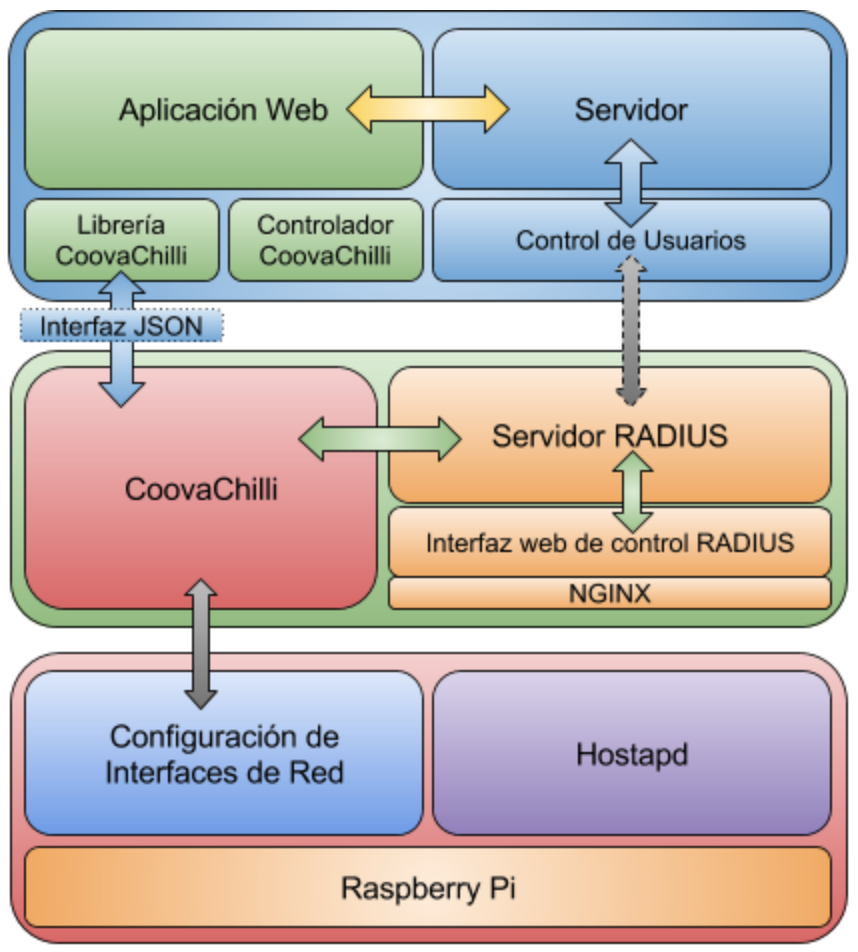
\includegraphics[width=0.75\linewidth]{./4_AnalisisFuncional/Img/modulosTotal.png}
\end{center}
\caption{Esquema completo de los módulos funcionales del sistema}
%\source{http://coova.github.io/CoovaChilli/}
\label{modulosTotal}
\end{figure}

Como también se adelantó en el anterior capítulo, Hostapd es un servicio que se ejecuta en segundo plano, configurando y permitiendo el uso de la interfaz inalámbrica \emph{wlan0} como punto de acceso WiFi 802.11n para que los clientes se conecten a nuestro servicio.

El submódulo \emph{Raspberry Pi}, con el sistema operativo Raspbian, proporciona las interfaces de red necesarias, \emph{software} y dependencias para instalar todo el ecosistema y las opciones de configuración de red que hacen posible la implementación total del servicio.

Para una mayor entendimiento global de todo el sistema instalado, configurado y desarrollado, en la Figura \ref{modulosTotal} se presenta un diagrama que engloba los tres módulos, incluyendo sus submódulos, y las interrelaciones existentes entre los mismos.
\cleardoublepage
\clearpage
\vspace*{\stretch{2}}
\begin{center}
\begin{minipage}{.75\textwidth}
\section{Análisis orgánico de la implantación del \emph{software}}

Una vez revisado el análisis previo y funcional del sistema de sensado móvil colaborativo mediante una visión \emph{top-down}, en este capítulo presentamos  el análisis orgánico de la implantación mediante una visión \emph{bottom-up}. Esto es, primero se configura el nivel inferior y el \emph{Control de Red}, tras lo cual se va ascendiendo en el modelo hasta llegar a la implantación del portal cautivo, en el nivel de \emph{Usuarios} y el nivel más alto del sistema. La descripción de la instalación del hardware se presenta en el Apéndice \ref{ApendiceA}.
\end{minipage}
\end{center}
\vspace{\stretch{3}} % \vfill % equivalent to \vspace{\fill}
\clearpage% https://tex.stackexchange.com/questions/70714/center-horizontally-and-vertically-a-block-of-text

\subsection{Módulos de Control de Red y de Acceso}
Una vez instalado Raspbian y arrancada con éxito la Raspberry Pi 3 (explicado en el Apéndice \ref{ApendiceA}), es necesario seguir configurando el ecosistema e instalando el \emph{software} necesario, idealmente mediante el gestor de paquetes y manejador de dependencias \emph{apt-get} y trabajando en todo momento desde el terminal \emph{bash}. Esto prepara el \emph{software} de los módulos \emph{Control de Red} y \emph{Control de Acceso}. Se detalla el procedimiento llevado a cabo en el mismo orden en el que se implementó en la práctica para que sea reproducible de forma sencilla la instalación de un nuevo sistema.

\subsubsection{Ajustes e instalaciones preliminares}
Una de las primeras configuraciones consiste en modificar el archivo \emph{/etc/network/interfaces} para introducir los detalles de nuestra red inalámbrica. Este paso prepara el submódulo \emph{Configuración de Interfaces Red} perteneciente al módulo de \emph{Control de Red}. En este TFG se ha utilizado la siguiente configuración de red para la interfaz inalámbrica \emph{wlan0}, que recordamos es la interfaz inalámbrica a la que se conectan eventualmente los usuarios del servicio.

\begin{listing}[H]
\begin{minted}
[
frame=lines,
framesep=2mm,
baselinestretch=1.2,
bgcolor=lightgray,
fontsize=\footnotesize,
breakanywhere,
breaklines=true,
breaksymbolleft={}
]
{bash}
auto wlan0
allow-hotplug wlan0
iface wlan0 inet static
    address 192.168.10.1
    netmask 255.255.255.0
    network 192.168.10.1
    post-up echo 1 > /proc/sys/net/ipv4/ip_forward
\end{minted}
\caption{Configuración de la interfaz de red wlan0}
\label{InterfacesConf}
\end{listing}

La última línea, \emph{post-up echo 1 > /proc/sys/net/ipv4/ip\_forward}, es la activación del \emph{flag} del \emph{kernel} que habilita el paso de datagramas IP tratados en la descripción del módulo de Control de Red. Si se prefiere utilizar esta orden de otra forma y así asegurarse de que el \emph{flag} queda activado también puede editarse el archivo \emph{/etc/sysctl.conf}, quitando el carácter de comentario (\emph{\#}) en la línea \emph{net.ipv4.ip\_forward=1} y reiniciando el servicio de red mediante la siguiente orden: \emph{/etc/init.d/networking restart}.

Una vez configurada la interfaz inalámbrica pueden instalarse los paquetes necesarios para preparar los módulos. Se incluyen algunos paquetes previos necesarios para la instalación posterior de \emph{software}, como herramientas para transferencia de datos (\emph{libcurl}), utilidades de red manejadas por CoovaChilli (\emph{iptables}), compiladores (\emph{gcc}) y gestores de dependencias para los mismos (\emph{make}). Recordamos que esta instalación debe ser realizada por el superusuario, por lo que se debe entrar en \emph{root} ejecutando primero la orden \emph{sudo su} o por el contrario utilizar la orden previa \emph{sudo} para cada orden a introducir. Además, pueden instalarse todos los paquetes necesarios con una sola orden escribiendo todos los nombres seguidos después de la orden \emph{apt-get install} y forzando una respuesta afirmativa a todas las preguntas que nos realice el terminal al instalar los paquetes usando los modificadores \emph{-y --force-yes}.

Los más relevantes para nuestro sistema son los paquetes \emph{freeradius} y \emph{mysql-server}, pero aquí se incluyen todos los instalados en la configuración de nuestro servicio:

\begin{listing}[H]
    \begin{minted}
    [
    frame=lines,
    framesep=2mm,
    baselinestretch=1.2,
    bgcolor=lightgray,
    fontsize=\footnotesize,
    breakanywhere,
    breaklines=true,
    breaksymbolleft={}
    ]
    {bash}
sudo apt-get install -y --force-yes debconf-utils
\end{minted}
\end{listing}

Con este primer paquete puede establecerse una contraseña para el usuario \emph{root} de la base de datos MySQL con las siguientes órdenes, a ejecutar después de que acabe el anterior, y sustituyendo la palabra CONTRASEÑA de las órdenes por la contraseña escogida. De esta forma, \emph{mysql-server} no pide una contraseña de \emph{root} en el momento de su instalación. Si no que se establece una contraseña diferente, la utilizada por defecto en la instalación de \emph{mysql-server} para Raspbian es \emph{raspbian}..

\begin{listing}[H]
    \begin{minted}
    [
    frame=lines,
    framesep=2mm,
    baselinestretch=1.2,
    bgcolor=lightgray,
    fontsize=\footnotesize,
    breakanywhere,
    breaklines=true,
    breaksymbolleft={}
    ]
    {bash}
echo 'mysql-server mysql-server/root_password password CONTRASEÑA' | debconf-set-selections
echo 'mysql-server mysql-server/root_password_again password CONTRASEÑA' | debconf-set-selections
\end{minted}
\end{listing}

Tras esto, ya pueden instalarse el resto de paquetes necesarios que habíamos comentado al principio.

\begin{listing}[H]
    \begin{minted}
    [
    frame=lines,
    framesep=2mm,
    baselinestretch=1.2,
    bgcolor=lightgray,
    fontsize=\footnotesize,
    breakanywhere,
    breaklines=true,
    breaksymbolleft={}
    ]
    {bash}
sudo apt-get install -y --force-yes debhelper libssl-dev libcurl4-gnutls-dev mysql-server freeradius freeradius-mysql gcc make libnl1 libnl-dev pkg-config iptables
\end{minted}
\end{listing}
La herramienta \emph{apt-get} instala también todos los paquetes de dependencias adicionales necesarias para el funcionamiento de los paquetes declarados.

Nótese que en este punto ya se ha empezado a instalar \emph{software} correspondiente al módulo de \emph{Control de Acceso}, como \emph{FreeRADIUS} y el servidor de bases de datos \emph{MySQL} con el que este va a funcionar. En el siguiente apartado se procede a su configuración.

\subsubsection{Configuración del Servidor RADIUS} \label{RADIUSConf}

Durante el paso anterior se instaló el servidor de base de datos MySQL y el servidor RADIUS. A continuación se procede a crear la base de datos a usar por el programa FreeRADIUS utilizando para ello unos \emph{scripts} proporcionados en su propia instalación.

Primero se crea la base de datos con la orden \emph{mysql}, utilizando el usuario root y la contraseña especificada anteriormente.

\begin{listing}[H]
    \begin{minted}
    [
    frame=lines,
    framesep=2mm,
    baselinestretch=1.2,
    bgcolor=lightgray,
    fontsize=\footnotesize,
    breakanywhere,
    breaklines=true,
    breaksymbolleft={}
    ]
    {bash}
echo 'create database radius' | mysql -u root -p CONTRASEÑA
\end{minted}
\end{listing}

Esto pone en marcha la interfaz de línea de órdenes de MySQL, con el usuario y contraseña detallados en las opciones, y le introduce el comando escrito entre comillas.

Tras esto, utilizamos una serie de \emph{scripts} que la instalación de FreeRADIUS ubica en su árbol de directorios y los introducimos como órdenes de MySQL para la base de datos \emph{radius} creada, de forma parecida a la utilizada en la última orden.

\begin{listing}[H]
\begin{minted}
[
frame=lines,
framesep=2mm,
baselinestretch=1.2,
bgcolor=lightgray,
fontsize=\footnotesize,
breakanywhere,
breaklines=true,
breaksymbolleft={}
]
{bash}
mysql -u root -p CONTRASEÑA radius < /etc/freeradius/sql/mysql/schema.sql
mysql -u root -p CONTRASEÑA radius < /etc/freeradius/sql/mysql/admin.sql
mysql -u root -p CONTRASEÑA radius < /etc/freeradius/sql/mysql/nas.sql
\end{minted}
\caption{Inserción de órdenes SQL desde ficheros de FreeRADIUS}
\label{RADIUSdatabaseScripts}
\end{listing}

Como opción antes de ejecutar estas órdenes, y para incrementar la seguridad, se puede modificar la contraseña por defecto de FreeRADIUS para operar en la base de datos (\emph{radpass}) en el archivo \emph{/etc/freeradius/sql/mysql/admin.sql}.

El siguiente paso es habilitar el soporte de SQL en el archivo de configuración de FreeRADIUS y como opción activar los contadores diarios. Para ello se debe editar el archivo ubicado en \emph{/etc/freeradius/radiusd.conf} y eliminando el carácter de comentario (\emph{\#}) de las líneas \emph{\$INCLUDE sql.conf}, \emph{\$INCLUDE sql/mysql/counter.conf} y opcionalmente de \emph{daily}.

Tras editar estos archivos, solo queda detener temporalmente la ejecución de FreeRADIUS, activar la autenticación SQL, comprobar que la configuración es correcta y volver a iniciar el servicio: \emph{service freeradius stop}.

Para activar la autenticación SQL hay que editar el archivo \emph{/etc/freeradius/sites-available/default} y quitar los comentarios de todas las líneas que contengan \emph{sql}. Una vez hecho esto comprobamos la configuración y reanudamos el servicio.

\begin{listing}[H]
    \begin{minted}
    [
    frame=lines,
    framesep=2mm,
    baselinestretch=1.2,
    bgcolor=lightgray,
    fontsize=\footnotesize,
    breakanywhere,
    breaklines=true,
    breaksymbolleft={}
    ]
    {bash}
freeradius -C
service freeradius start
\end{minted}
\end{listing}

En este punto FreeRADIUS aún no ha terminado del todo su configuración, pero para ello es necesario que acaben las instalaciones de los demás componentes.

\subsubsection{Instalación de CoovaChilli} \label{CoovaInstall}

Llegados a este punto podemos instalar y configurar el núcleo de funcionamiento de nuestro sistema, que es el servicio CoovaChilli. Como se comentó anteriormente, este \emph{software} es un proyecto de código abierto basado en una antigua solución propietaria. Lamentablemente, su código no se encuentra disponible en forma de paquete precompilado que se pueda instalar mediante un orden sencillo con el gestor de paquetes \emph{apt-get}, sino que se ha de descargar el código fuente y compilarlo manualmente, convirtiéndolo en un paquete .deb instalable de forma manual en sistemas basados en Debian. En este TFG se ha utilizado el código fuente de la aplicación alojado en GitHub, que permite dicha compilación, descargándolo mediante la herramienta de control de versiones git que ha de estar instalada en nuestro sistema operativo.

Como sucedió con el paso de FreeRADIUS, deben realizarse unas instalaciones previas de paquetes y dependencias auxiliares antes de comenzar la propia instalación de CoovaChilli y los demás elementos de \emph{software}, entre los que se encuentra \emph{git}.

\begin{listing}[H]
    \begin{minted}
    [
    frame=lines,
    framesep=2mm,
    baselinestretch=1.2,
    bgcolor=lightgray,
    fontsize=\footnotesize,
    breakanywhere,
    breaklines=true,
    breaksymbolleft={}
    ]
    {bash}
apt-get install -y --force-yes git libjson-c-dev haserl gengetopt devscripts libtool bash-completion autoconf automake
\end{minted}
\end{listing}

Tras esto, hay que descargar el código fuente de CoovaChilli en un directorio y compilarlo en un paquete instalable en Debian, que puede lograrse con una utilidad del sistema operativo en unas pocas líneas. Este último proceso de compilación puede llevar tiempo y si no está todo previamente instalado y configurado puede fallar.

\begin{listing}[H]
    \begin{minted}
    [
    frame=lines,
    framesep=2mm,
    baselinestretch=1.2,
    bgcolor=lightgray,
    fontsize=\footnotesize,
    breakanywhere,
    breaklines=true,
    breaksymbolleft={}
    ]
    {bash}
cd /usr/src
git clone https://github.com/coova/coova-chilli.git
\end{minted}
\end{listing}

Tras acabar el proceso de descarga, comenzamos el proceso de compilación situándonos en la raíz del código fuente recién descargado con la línea anterior.

\begin{listing}[H]
    \begin{minted}
    [
    frame=lines,
    framesep=2mm,
    baselinestretch=1.2,
    bgcolor=lightgray,
    fontsize=\footnotesize,
    breakanywhere,
    breaklines=true,
    breaksymbolleft={}
    ]
    {bash}
cd /usr/src/coova-chilli
dpkg-buildpackage -us -uc
\end{minted}
\end{listing}

En este punto comienza la compilación del código fuente. Al finalizar, tendríamos un archivo de nombre similar a \emph{coova-chilli\_1.3.0\_armhf.deb} en el directorio \emph{/usr/src/} y podríamos proceder a instalarlo situándonos en dicho directorio y utilizando el gestor de paquetes \emph{dpkg}.

\begin{listing}[H]
    \begin{minted}
    [
    frame=lines,
    framesep=2mm,
    baselinestretch=1.2,
    bgcolor=lightgray,
    fontsize=\footnotesize,
    breakanywhere,
    breaklines=true,
    breaksymbolleft={}
    ]
    {bash}
cd /usr/src
dpkg -i coova-chilli_1.3.0_armhf.deb
\end{minted}
\end{listing}

\paragraph{Configuración Inicial de CoovaChilli} \label{CoovaConfig} ~\\

Llegados a este punto el programa CoovaChilli está instalado y podemos proceder a su configuración. Esta configuración en su mayoría se basa, como se adelantó en la descripción del \emph{software} del anterior capítulo, en modificar el archivo \emph{/etc/chilli/defaults} o hacer una copia de éste bajo el nombre \emph{config} teniendo allí las modificaciones con respecto a \emph{defaults}. Sin embargo, hay dos pasos previos a la configuración de este archivo.

En primer lugar debemos modificar el \emph{script} que CoovaChilli ejecuta al ponerse en marcha la interfaz TUN (ubicado en \emph{/etc/chilli/up.sh}) introduciendo una regla de la herramienta \emph{iptables} para permitir el reenvío de los paquetes IP desde la interfaz de red cableada \emph{eth0}, que se almacena en una variable interna de la configuración de CoovaChilli llamada \emph{HS\_WANIF}.

\begin{listing}[H]
    \begin{minted}
    [
    frame=lines,
    framesep=2mm,
    baselinestretch=1.2,
    bgcolor=lightgray,
    fontsize=\footnotesize,
    breakanywhere,
    breaklines=true,
    breaksymbolleft={}
    ]
    {bash}
    iptables -I POSTROUTING -t nat -o $HS_WANIF -j MASQUERADE
    \end{minted}
    \end{listing}

También debemos activar el \emph{flag} que permite activar CoovaChilli en el archivo \emph{/etc/default/chilli/} cambiando el valor de la variable \emph{START\_CHILLI} de 0 a 1.

Tras esto, se debe editar el archivo de configuración de CoovaChilli introduciendo los valores adecuados a nuestro sistema en los atributos relevantes en este momento en el archivo \emph{/etc/chilli/defaults} o bien en su copia renombrada como \emph{/etc/chilli/config}, que al iniciar el sistema reemplaza los valores dados en defaults donde difieran. Dado que en este momento aún no se encuentra instalada la herramienta \emph{hostapd} (ver más adelante) aún no tenemos habilitado un SSID para nuestro sistema, por lo que en un paso posterior tras la instalación de \emph{hostapd} debemos volver a este archivo de configuración e introducir el nombre del SSID que hayamos establecido. En el caso de este TFG, el SSID utilizado es \emph{RasPiDav}.

\begin{listing}[H]
\begin{minted}
[
frame=lines,
framesep=2mm,
baselinestretch=1.2,
bgcolor=lightgray,
fontsize=\footnotesize,
breaklines=true,
breaksymbolleft={}
]
{bash}
HS_WANIF=eth0
HS_LANIF=wlan0
HS_NETWORK=192.168.10.0
HS_UAMLISTEN=192.168.10.1
HS_UAMALLOW=192.168.10.0
HS_SSID=RasPiDav
HS_COAPORT=3799
HS_UAMSECRET=
\end{minted}
\caption{Configuración de CoovaChilli}
\label{CoovaConf}
\end{listing}

Debido al funcionamiento de nuestro portal cautivo, que opera con la interfaz JSON de CoovaChilli, es necesario dejar en blanco el campo \emph{HS\_UAMSECRET}, de lo contrario la aplicación Web no podría iniciar sesión en el servicio con las credenciales obtenidas.

\paragraph{Instalación de Haserl} \label{HaserlInstallTitle} ~\\

Dado que algunas de las funciones de CoovaChilli necesitan del programa Haserl (como su pequeño portal cautivo por defecto implementado con \emph{Web Scripts}) hace falta instalarlo y añadir su ruta de instalación a la configuración de CoovaChilli. Para ello hacemos un procedimiento similar al usado en la instalación de CoovaChilli, salvo que en este caso compilamos el programa con la utilidad \emph{make}.

\begin{listing}[H]
\begin{minted}
[
frame=lines,
framesep=2mm,
baselinestretch=1.2,
bgcolor=lightgray,
fontsize=\footnotesize,
breaklines=true,
breaksymbolleft={}
]
{bash}
cd /usr/src
wget http://downloads.sourceforge.net/project/haserl/haserl-devel/haserl-0.9.35.tar.gz
tar zxvf  haserl-0.9.35.tar.gz
cd /usr/src/haserl-0.9.35
./configure
make
make install
\end{minted}
\caption{Instalando Haserl}
\label{HaserlInstall}
\end{listing}

Tras esto actualizamos la ruta de \emph{Haserl} para CoovaChilli en el archivo \emph{/etc/chilli/wwwsh} buscando la línea \emph{haserl=} y modificándola a \emph{haserl=/usr/local/bin/haserl}. Tras esto, solo queda poner en marcha CoovaChilli con la siguiente orden.

\begin{listing}[H]
    \begin{minted}
    [
    frame=lines,
    framesep=2mm,
    baselinestretch=1.2,
    bgcolor=lightgray,
    fontsize=\footnotesize,
    breakanywhere,
    breaklines=true,
    breaksymbolleft={}
    ]
    {bash}
service chilli start
\end{minted}
\end{listing}

\subsubsection{Instalación y configuración de Hostapd} \label{HostapdInstallConfig}

En este momento se prepara la herramienta \emph{hostapd} para poner en marcha la interfaz WiFi como Punto de Acceso IEEE 802.11n, comenzando por su instalación y continuando con su configuración.

\begin{listing}[H]
    \begin{minted}
    [
    frame=lines,
    framesep=2mm,
    baselinestretch=1.2,
    bgcolor=lightgray,
    fontsize=\footnotesize,
    breakanywhere,
    breaklines=true,
    breaksymbolleft={}
    ]
    {bash}
apt-get install -y --force-yes hostapd
\end{minted}
\end{listing}

Cuando termine la instalación se edita el archivo de configuración \emph{/etc/default/hostapd} añadiendo la ruta del archivo de configuración que contiene los atributos deseados para nuestro punto de acceso, que está ubicado en \emph{/etc/hostapd/hostapd.conf}. Para ello buscamos la línea que contenga \emph{DAEMON\_CONF=}, nos aseguraremos de que está sin comentar y le especificaremos la ruta entre comillas, de manera que quede de la siguiente forma: \emph{DAEMON\_CONF=``/etc/hostapd/hostapd.conf''}.

Ahora configuramos el mismo archivo cuya ruta hemos indicado en el ajuste anterior, indicando todos los atributos para nuestro punto de acceso incluyendo el driver a utilizar (\emph{nl80211}). Recordamos que la interfaz establecida ha de ser la misma que indicamos en el archivo de configuración \emph{defaults} o \emph{config} de CoovaChilli como \emph{HS\_LANIF}, en nuestro caso \emph{wlan0}, que tiene la red estática ya configurada en el archivo interfaces al principio de la implantación. Además, el SSID también ha de ser el mismo que indicamos a CoovaChilli con la variable \emph{HS\_SSID}.

\begin{listing}[H]
\begin{minted}
[
frame=lines,
framesep=2mm,
baselinestretch=1.2,
bgcolor=lightgray,
fontsize=\footnotesize,
breaklines=true,
breaksymbolleft={}
]
{bash}
interface=wlan0
driver=nl80211
ssid=RasPiDav
hw_mode=g
channel=6
auth_algs=1
beacon_int=100
dtim_period=2
max_num_sta=255
rts_threshold=2347
fragm_threshold=2346
ieee80211n=1
wmm_enabled=1
ht_capab=[HT40][SHORT-GI-20][DSSS_CCK-40]
\end{minted}
\caption{Configuración de Hostapd}
\label{HostapdConf}
\end{listing}

En este punto reiniciamos hostapd para que utilice los ajustes deseados. Al ejecutar este orden ya sería visible la red WiFi de la Raspberry Pi 3 (Figura \ref{redesVisibles}) desde otros dispositivos con el SSID indicado:

\begin{listing}[H]
    \begin{minted}
    [
    frame=lines,
    framesep=2mm,
    baselinestretch=1.2,
    bgcolor=lightgray,
    fontsize=\footnotesize,
    breakanywhere,
    breaklines=true,
    breaksymbolleft={}
    ]
    {bash}
    service hostapd start
    \end{minted}
    \end{listing}

\begin{figure}[!t]
\begin{center}
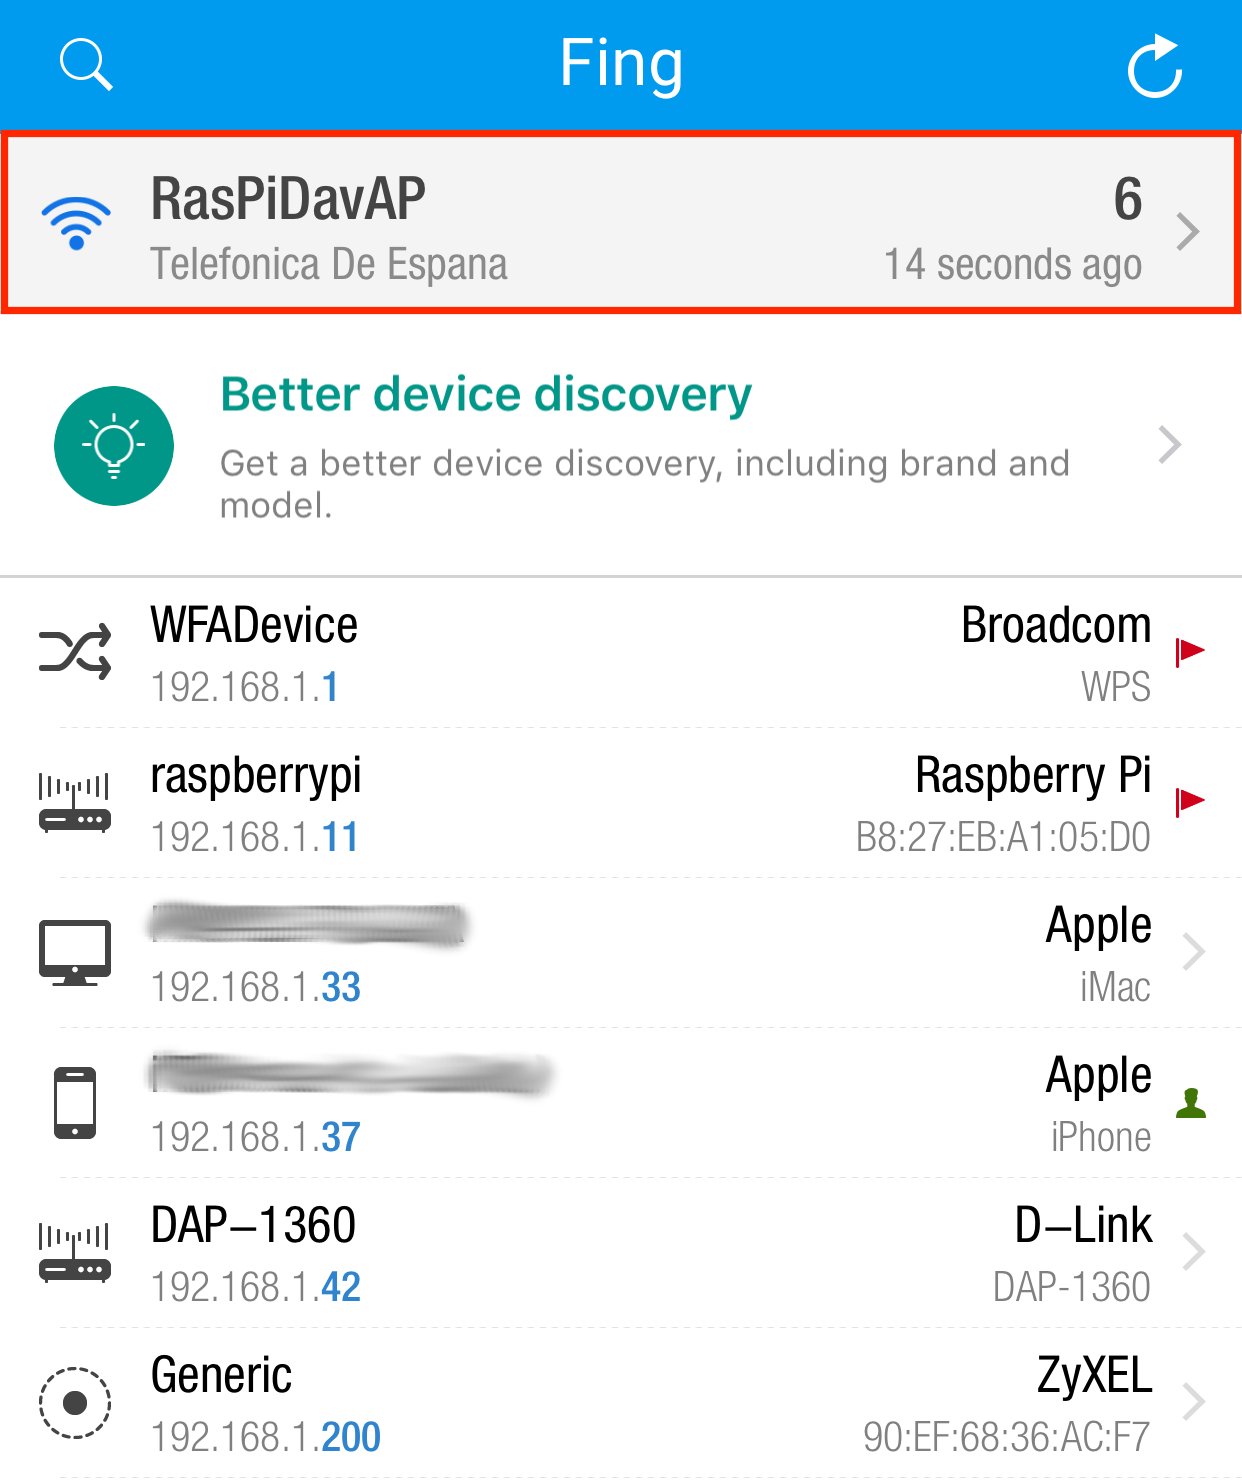
\includegraphics[width=0.75\linewidth]{./5_AnalisisOrganico/Img/redesVisibles.png}
\end{center}
\caption{Ventana que muestra todas las redes WiFi disponibles y entre ellas la que hemos configurado (en este caso RasPiDavAP, recuadrada en rojo)}
% \source{http://coova.github.io/CoovaChilli/}
\label{redesVisibles}
\end{figure}

\subsubsection{La interfaz Web de daloRADIUS} \label{daloRADIUSInstall}

Para facilitar la administración del servicio, incluyendo la gestión del servidor RADIUS, puede resultar útil implementar servicios que ofrecen interfaces gráficas fáciles de comprender y manejar. Para hacer uso de uno de los servicios de este tipo más conocidos para FreeRADIUS, conocido como daloRADIUS, instalamos el servidor Web NGINX y alojamos allí los archivos necesarios para gestionar el servidor RADIUS desde una aplicación tan sencilla y ubicua como el navegador Web.

En primer lugar, instalamos el servidor Web y las herramientas necesarias para utilizar daloRADIUS, que son sobre todo librerías de soporte PHP.

\begin{listing}[H]
    \begin{minted}
    [
    frame=lines,
    framesep=2mm,
    baselinestretch=1.2,
    bgcolor=lightgray,
    fontsize=\footnotesize,
    breakanywhere,
    breaklines=true,
    breaksymbolleft={}
    ]
    {bash}
    apt-get install -y --force-yes php5-mysql php-pear php5-gd php-db php5-fpm libgd2-xpm-dev libpcrecpp0 libxpm4 nginx php5-xcache
    \end{minted}
\end{listing}

Cuando acabe esta instalación el programa \emph{NGINX} queda instalado y podríamos alojar el contenido Web que deseamos servir en el directorio \emph{/usr/share/nginx/html/}. En nuestro caso, descargamos los contenidos de daloRADIUS, los descomprimimos allí y renombramos el directorio generado para acceder a él al teclear la futura URL desde el navegador.

\begin{listing}[H]
\begin{minted}
[
frame=lines,
framesep=2mm,
baselinestretch=1.2,
bgcolor=lightgray,
fontsize=\footnotesize,
breaklines=true,
breaksymbolleft={}
]
{bash}
cd /usr/src
wget https://sourceforge.net/projects/daloradius/files/latest/download
tar zxvf download -C /usr/share/nginx/html/
mv /usr/share/nginx/html/daloradius-0.9-9 /usr/share/nginx/html/daloradius
\end{minted}
\caption{Instalando daloRADIUS}
\label{daloRADIUS}
\end{listing}

Aunque no los usamos en este TFG, conviene remarcar que daloRADIUS también incluye portales cautivos de ejemplo para ser usados con \emph{CoovaChilli} en el árbol de directorios que hemos descomprimido y renombrado, implementados usando PHP y JavaScript. Tras nuestros cambios, estos portales cautivos quedan ubicados en la ruta \emph{/usr/share/nginx/html/daloradius/contrib/chilli/}.

La descarga de daloRADIUS contiene archivos específicos que lo habilitan para ser usado con \emph{FreeRADIUS} y \emph{MySQL}. Para utilizarlos debemos copiar dichos archivos existentes en el árbol de directorios de \emph{daloRADIUS} y colocarlos en los directorios de \emph{FreeRADIUS} indicados en las siguientes órdenes, reemplazando las originales. Por seguridad conviene detener el servicio \emph{FreeRADIUS} antes de modificar archivos y hacer copia de seguridad de los archivos que quedan reemplazados, renombrándolos o cambiando las extensiones.

\begin{listing}[H]
\begin{minted}
[
frame=lines,
framesep=2mm,
baselinestretch=1.2,
bgcolor=lightgray,
fontsize=\footnotesize,
breaklines=true,
breakanywhere,
breaksymbolleft={}
]
{bash}
service freeradius stop
cp /usr/share/nginx/html/daloradius/contrib/configs/freeradius-2.1.8/cfg1/raddb/sql/mysql/counter.conf /etc/freeradius/sql/mysql/counter.conf
cp /usr/share/nginx/html/daloradius/contrib/configs/freeradius-2.1.8/cfg1/raddb/sites-available/default /etc/freeradius/sites-available/default
cp /usr/share/nginx/html/daloradius/contrib/configs/freeradius-2.1.8/cfg1/raddb/modules/sql.conf /etc/freeradius/sql.conf
\end{minted}
\caption{Configuración de daloRADIUS para trabajar con FreeRADIUS}
\label{RADIUSdatabases}
\end{listing}

Dado que el último archivo que hemos ubicado (\emph{/etc/freeradius/sql.conf}) procede de una instalación nueva de daloRADIUS contiene la contraseña utilizada por defecto en FreeRADIUS, por lo que debemos editarlo para que tenga la contraseña que indicamos en el paso correspondiente del apartado \ref{RADIUSConf}. Recordamos que, si no se cambió, la contraseña utilizada por defecto es \emph{radpass}.

Tras estos pasos podemos iniciar el servidor RADIUS de nuevo y utilizar el \emph{script} específico de \emph{daloRADIUS} incluido en la instalación para añadir la configuración de \emph{daloRADIUS} en MySQL, añadiendo también los permisos de usuario correspondientes para poder manejar el servidor. Recordamos que la palabra CONTRASEÑA en mayúscula en este caso hace referencia a la contraseña utilizada para el usuario \emph{root} del servidor MySQL.

\begin{listing}[H]
\begin{minted}
[
frame=lines,
framesep=2mm,
baselinestretch=1.2,
bgcolor=lightgray,
fontsize=\footnotesize,
breaklines=true,
breaksymbolleft={}
]
{bash}
service freeradius start
mysql -u root -p CONTRASEÑA radius < /usr/share/nginx/html/daloradius/contrib/db/fr2-mysql-daloradius-and-freeradius.sql
echo "GRANT ALL ON radius.* to 'radius'@'localhost';" > /tmp/grant.sql
echo "GRANT ALL ON radius.* to 'radius'@'127.0.0.1';" >> /tmp/grant.sql
mysql -u root -p CONTRASEÑA < /tmp/grant.sql
\end{minted}
\caption{Creando bases de datos para daloRADIUS}
\label{daloRADIUSdatabases}
\end{listing}

Además, actualizamos el archivo de daloRADIUS que contiene el usuario y contraseña de la base de datos para que tenga el usuario y contraseña del servidor RADIUS. Este archivo está en \emph{/usr/share/nginx/html/daloradius/library/daloradius.conf.php} y ha de tener los siguientes valores en los campos correspondientes. Recordamos que esta contraseña es la del servidor RADIUS, indicada por CONTRASEÑA-RADIUS, (por defecto \emph{radpass} si no la cambiamos).

\begin{listing}[H]
    \begin{minted}
    [
    frame=lines,
    framesep=2mm,
    baselinestretch=1.2,
    bgcolor=lightgray,
    fontsize=\footnotesize,
    breakanywhere,
    breaklines=true,
    breaksymbolleft={}
    ]
    {bash}
$configValues['CONFIG_DB_USER'] = 'radius';
$configValues['CONFIG_DB_PASS'] = 'CONTRASEÑA-RADIUS';
\end{minted}
\end{listing}

\paragraph{Configurando NGINX para servir daloRADIUS} \label{NGINXdaloRADIUS} ~\\

Tras preparar \emph{daloRADIUS} para su funcionamiento hemos de configurar el servidor NGINX para que nos sirva la página principal correcta al introducir la ruta adecuada en el navegador. Para esta configuración editamos el archivo \emph{/etc/nginx/sites-available/default} añadiendo la siguiente directriz de servidor. Para acceder a la interfaz Web en el futuro utilizamos el puerto 80.

\begin{listing}[H]
\begin{minted}
[
frame=lines,
framesep=2mm,
baselinestretch=1.2,
bgcolor=lightgray,
fontsize=\footnotesize,
breaklines=true,
breaksymbolleft={}
]
{bash}
server {
           listen 80 default_server;
           listen [::]:80 default_server;
           root /usr/share/nginx/html;
           index index.html index.htm index.php;
           server_name _;
           location / {
               try_files $uri $uri/ =404;
           }
           location ~ \.php$ {
               include snippets/fastcgi-php.conf;
               fastcgi_pass unix:/var/run/php5-fpm.sock;
           }
}
\end{minted}
\caption{Directriz de servidor de NGINX para daloRADIUS}
\label{directiveNGINX}
\end{listing}

Llegados a este punto solo queda comprobar que la configuración de NGINX es la correcta y reiniciar tanto el servidor Web como \emph{hostapd}.

\begin{listing}[H]
    \begin{minted}
    [
    frame=lines,
    framesep=2mm,
    baselinestretch=1.2,
    bgcolor=lightgray,
    fontsize=\footnotesize,
    breakanywhere,
    breaklines=true,
    breaksymbolleft={}
    ]
    {bash}
nginx -t
service nginx restart
service hostapd restart
\end{minted}
\end{listing}

Tras esto podemos acceder a \emph{daloRADIUS} desde el navegador para realizar las gestiones deseadas utilizando la IP proporcionada a la interfaz cableada. Por ejemplo, si la IP de dicha interfaz es 192.168.1.30 se puede acceder a \emph{daloRADIUS} accediendo a la URL \emph{http://192.168.1.30/daloradius/}.

\paragraph{Utilizando daloRADIUS para añadir a los usuarios del servicio} \label{daloRADIUSusers} ~\\

Una vez terminada nuestra instalación solo queda añadir usuarios al servidor RADIUS para que puedan conectarse al servicio, usando para ello el portal cautivo cuya implantación veremos en los siguientes apartados. Gracias a la instalación de \emph{daloRADIUS} podemos añadir estos usuarios de forma gráfica a través del navegador Web en lugar de utilizar órdenes SQL desde un terminal. Cuando accedamos a \emph{daloRADIUS} accediendo a la URL descrita anteriormente se carga una vista similar a la de la Figura \ref{daloLogin}.

\begin{figure}[!t]
\begin{center}
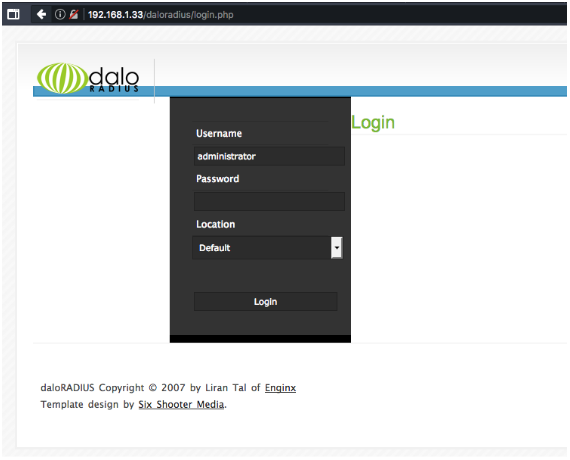
\includegraphics[width=0.75\linewidth]{./5_AnalisisOrganico/Img/daloLogin.png}
\end{center}
\caption{Vista de la página de entrada a daloRADIUS}
% \source{http://coova.github.io/CoovaChilli/}
\label{daloLogin}
\end{figure}

El usuario \emph{administrator} está ya escrito en el campo \emph{Username}. La contraseña para dicho usuario, a escribir en el campo inferior, es \emph{radius}. Al hacer clic en el botón \emph{Login} entramos en la pantalla principal de daloRADIUS (Figura \ref{daloMain}).

\begin{figure}[!t]
\begin{center}
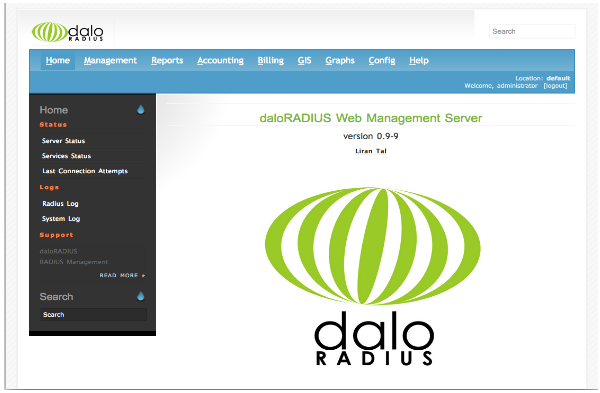
\includegraphics[width=0.75\linewidth]{./5_AnalisisOrganico/Img/daloMain.png}
\end{center}
\caption{Vista principal de daloRADIUS}
% \source{http://coova.github.io/CoovaChilli/}
\label{daloMain}
\end{figure}

Aquí hacemos clic en la pestaña \emph{Management} del menú superior y tras ello en la opción \emph{New User} del menú lateral izquierdo, lo que nos conduce al formulario de añadir nuevo usuario que nos permite escoger el tipo de autenticación a utilizar. En nuestro caso es la primera opción, \emph{Username Authentication} (Figura \ref{daloNewUser}).

\begin{figure}[!t]
\begin{center}
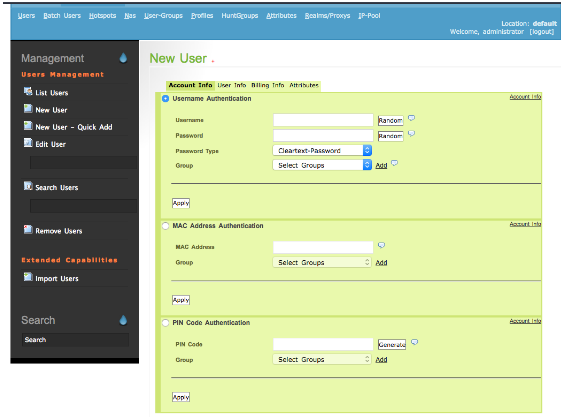
\includegraphics[width=0.75\linewidth]{./5_AnalisisOrganico/Img/daloNewUser.png}
\end{center}
\caption{Vista de la página de manejo de usuarios en daloRADIUS}
% \source{http://coova.github.io/CoovaChilli/}
\label{daloNewUser}
\end{figure}

Pulsando el botón \emph{Apply} tras haber rellenado los campos se completa el proceso de creación de usuario. Haciendo clic en el elemento \emph{List Users} del menú lateral izquierdo podemos ver una lista de los usuarios registrados en el servicio y varios menús desplegables con detalles sobre los mismos.

Además de registrar usuarios es posible asignarlos en grupos y modificar algunos atributos, por ejemplo el tiempo de conexión, máximo volumen de datos a transferir o incluso el intervalo de tiempo en el que es posible conectarse. Dichos atributos pertenecen a \emph{FreeRADIUS}, aunque \emph{daloRADIUS} permite usar atributos y variables de otros fabricantes, y pueden cambiarse en la pestaña \emph{Attributes} al crear un nuevo usuario o seleccionar uno ya existente de la lista (Figura \ref{daloAttributes}).

\begin{figure}[!t]
\begin{center}
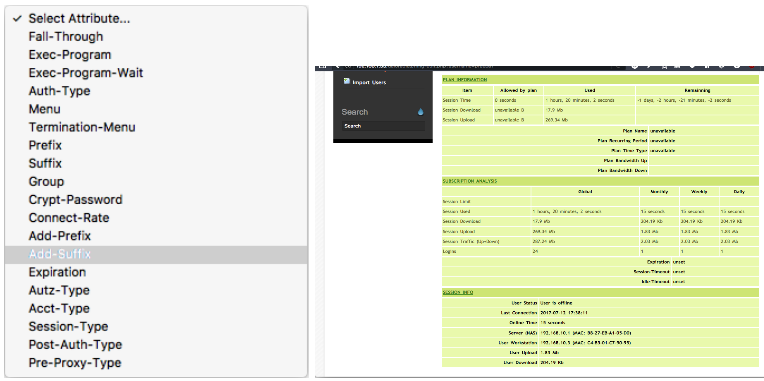
\includegraphics[width=0.75\linewidth]{./5_AnalisisOrganico/Img/daloAttributes.png}
\end{center}
\caption{Vista de la página de Attributes de daloRADIUS}
% \source{http://coova.github.io/CoovaChilli/}
\label{daloAttributes}
\end{figure}

Para añadir usuarios en bloque, daloRADIUS ofrece un modo de añadir conjuntos completos de usuarios, facilitando en gran parte el proceso de población de la base de datos. Para ello, en el submenú \emph{Management} puede seleccionarse la opción \emph{Batch Users}, tras lo cual la opción de añadir usuarios en bloque, consultarlos o eliminarlos queda disponible en la barra lateral izquierda. Es posible gestionar el modo en que se generan los nombres de usuario, la longitud de los caracteres utilizados, el número de instancias o los grupos a los que pertenecerán. Este conjunto de usuarios, recién creado, puede exportarse a un archivo Excel y \emph{Comma Separated Values} (\acrshort{CSV}), que pueden ser pasados a un \emph{parser} que pase los pares usuario-contraseña a otro formato, como se ha hecho en este TFG, o incluso imprimirse en forma de tarjetas para entregar a posibles usuarios (Figura \ref{daloBatchUsers}).

\begin{figure}[!t]
\begin{center}
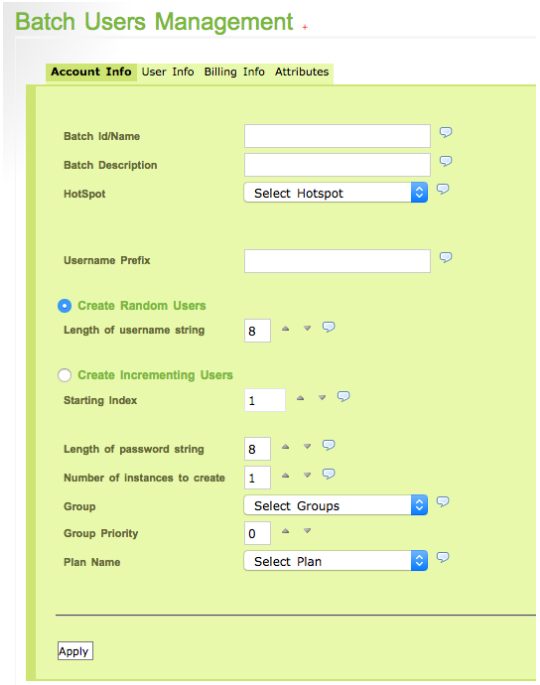
\includegraphics[width=0.75\linewidth]{./5_AnalisisOrganico/Img/daloBatchUsers.png}
\end{center}
\caption{Vista de la página de entrada a daloRADIUS por lotes}
% \source{http://coova.github.io/CoovaChilli/}
\label{daloBatchUsers}
\end{figure}

Para implantar dos tipos de usuarios, el caso de este TFG, donde hay un conjunto de usuarios que solo tienen un tiempo de conexión de 30 m, puede crearse un segundo conjunto de usuarios que cuenten con dicha restricción haciendo uso del atributo \emph{RADIUS Session-Timeout} definido en la RFC 2865. Tras seleccionar el atributo se le asigna el valor buscado medido en segundos (Figura \ref{daloBatchUsersMan}).

\begin{figure}[!t]
\begin{center}
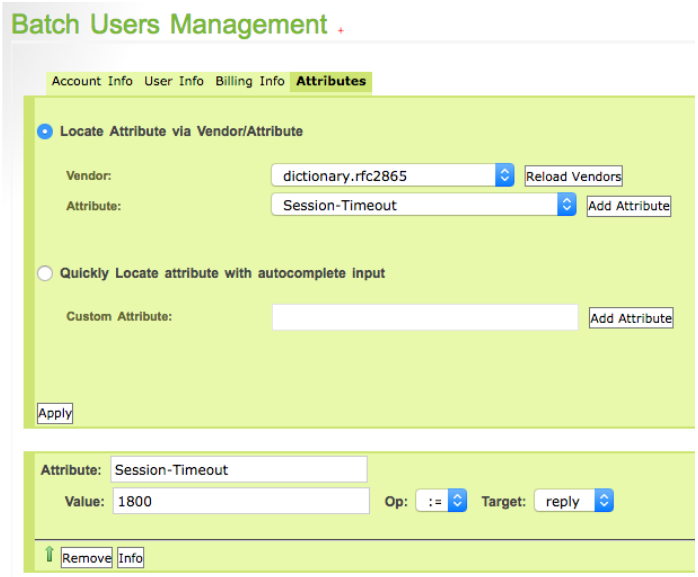
\includegraphics[width=0.75\linewidth]{./5_AnalisisOrganico/Img/daloBatchUsersMan.png}
\end{center}
\caption{Vista de la página de RADUIS Session-timeout de daloRADIUS}
% \source{http://coova.github.io/CoovaChilli/}
\label{daloBatchUsersMan}
\end{figure}

\subsection{Módulo de Usuarios}
A diferencia de los dos módulos anteriores, cuya implantación se basa únicamente en la instalación y configuración de \emph{software}, el módulo de usuarios cuenta con un mayor esfuerzo de programación, encontrándose el módulo en su totalidad contenido en único directorio del sistema constituido por archivos JavaScript, JSON, HTML y CSS. A continuación analizamos la implantación general y de cada uno de los submódulos que constituyen el módulo de usuarios, sobre todo aquellos que han sido programados desde cero, entrando en un mayor detalle sobre sus funciones individuales.

\subsubsection{Configuración previa y estructura del módulo} \label{userModuleConfig}
Dado que el módulo de usuarios basa su funcionamiento en Node.js y npm debemos instalar estos dos componentes, pues habitualmente la versión de los mismos incluida por defecto en los sistemas operativos Linux es muy antigua. Los pasos necesarios para descargar e instalar ambas utilidades varían según el sistema operativo. En nuestro caso, Node.js no está incluido por defecto en los repositorios por lo que en principio no puede instalarse con un sencillo comando de \emph{apt-get}. Podemos añadir un repositorio de su última versión para su fácil instalación y actualización con un único paso previo desde el terminal, tras el cual podremos instalarlo siguiendo el procedimiento habitual.

\begin{listing}[H]
    \begin{minted}
    [
    frame=lines,
    framesep=2mm,
    baselinestretch=1.2,
    bgcolor=lightgray,
    fontsize=\footnotesize,
    breakanywhere,
    breaklines=true,
    breaksymbolleft={}
    ]
    {bash}
curl -sL https://deb.nodesource.com/setup_8.x | sudo -E bash -
sudo apt-get install -y nodejs
    \end{minted}
\end{listing}

Este procedimiento instala tanto Node.js como el gestor de paquetes npm, permitiendo su ejecución desde terminal con las órdenes \emph{node} y \emph{npm} respectivamente.

Se ha implementado el módulo de usuarios completo en un único directorio. En la Figura \ref{repoGitHub} se adjunta una imagen con la estructura del mismo sacada directamente del repositorio alojado en \emph{GitHub}.

\begin{figure}[!t]
\begin{center}
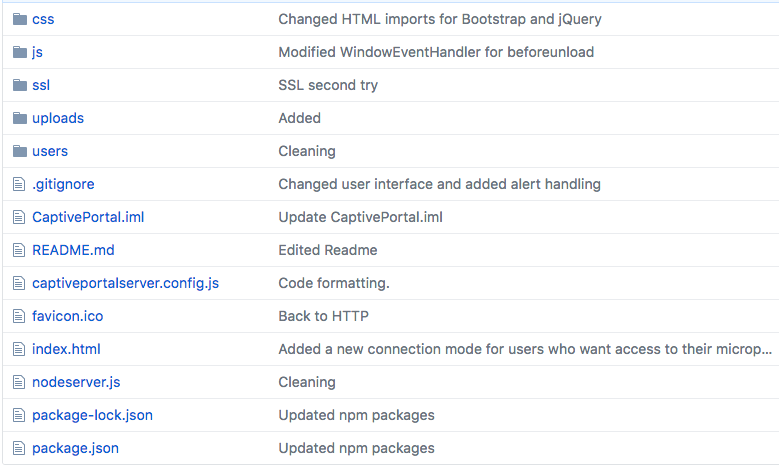
\includegraphics[width=0.75\linewidth]{./5_AnalisisOrganico/Img/repoGitHub.png}
\end{center}
\caption{Imagen de la estructura del directorio en el que se incluye el código programado para el módulo Usuario}
% \source{http://coova.github.io/CoovaChilli/}
\label{repoGitHub}
\end{figure}

%A excepción de los directorios scripts y csvgen y del archivo CaptivePortal.iml, correspondientes respectivamente a utilidades de configuración y archivos propios del \emph{software} de trabajo, c
Cada archivo o directorio está directamente relacionado con uno de los submódulos, quedando distribuidos de la siguiente forma.

\begin{itemize}
\item \emph{Control de Usuarios}: directorio \emph{users} y todos sus archivos.
\item \emph{Servidor}: archivos \emph{nodeserver.js}, \emph{captiveportalserver.config.js}, \emph{package.json} y \emph{package-lock.json} y directorio \emph{uploads}.
\item \emph{Aplicación Web}: archivos \emph{index.html} y directorios \emph{js}, \emph{css}, \emph{ssl} y todos sus archivos.
\end{itemize}

El funcionamiento de dicho módulo y las interrelaciones existentes entre sus submódulos se adelantaron en secciones anteriores de este capítulo. El diagrama de secuencia de la Figura \ref{diagramUML} muestra la interacción de la aplicación Web (\emph{Web App}), el servidor (\emph{Server}) y el las acciones que puede hacer el usuario (\emph{User Ctrl}).

\begin{figure}[!t]
\begin{center}
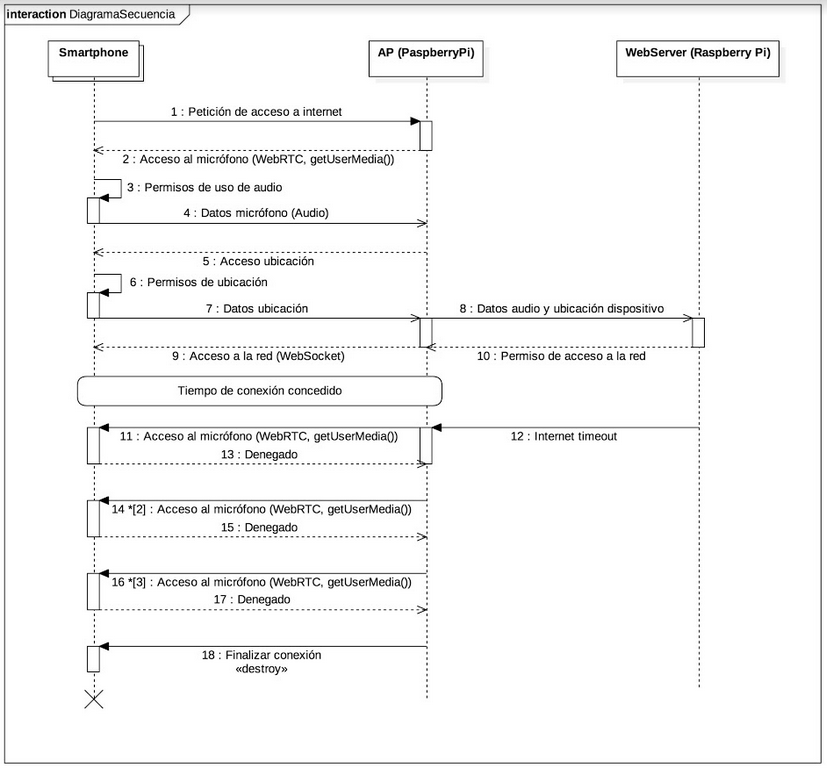
\includegraphics[width=0.75\linewidth]{./5_AnalisisOrganico/Img/diagramUML.png}
\end{center}
\caption{Diagrama de secuencia de los componentes del módulo de Usuario}
% \source{http://coova.github.io/CoovaChilli/}
\label{diagramUML}
\end{figure}


Donde las auto-interacciones 5, 6 y 7 son pedidas al usuario y las 13 y 16 son llevadas a cabo a través de la interfaz JSON de \emph{CoovaChilli}. Sobre este último aspecto se profundiza más adelante.

\subsubsection{Submódulo de Control Usuarios} \label{userControl}

Como ya adelantamos, en cuanto a estructura de directorios, el submódulo de control de usuarios está totalmente contenido en el directorio \emph{users} de nuestro módulo de Usuario. Consta de cuatro archivos: dos bases de datos de usuarios JSON (\emph{users.json} y \emph{usersOneTime.json}) y los archivos JavaScript que controlan dichas bases de datos (\emph{userController.js} y \emph{userControllerOneTime.js}). Los archivos con el sufijo \emph{--OneTime} en el nombre indican que son la base de datos y controlador correspondientes a la opción de conectarse durante 30 minutos a cambio de un único archivo de audio (Figura \ref{usersDir}).

\begin{figure}[!t]
\begin{center}
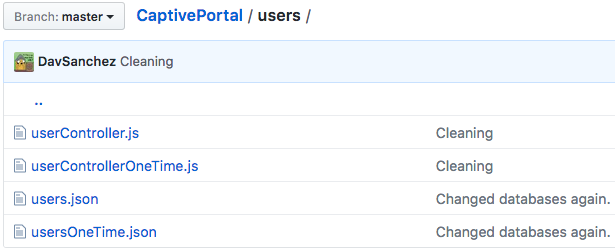
\includegraphics[width=0.75\linewidth]{./5_AnalisisOrganico/Img/usersDir.png}
\end{center}
\caption{Vista del directorio con los archivos del submódulo Control de Usuarios}
% \source{http://coova.github.io/CoovaChilli/}
\label{usersDir}
\end{figure}

Si la base de usuarios se vuelve lo suficientemente grande y soporta una carga mucho mayor que la existente en las pruebas realizadas en este TFG este módulo podría reemplazarse por una herramienta de base de datos más potente a utilizar (SQL, MongoDB) o incluso dejar de ser un submódulo separado del propio servidor RADIUS del módulo de control de acceso, permitiendo al servidor trabajar directamente con la base de datos de FreeRADIUS.

Dado que cuatro los archivos constituyen dos pares muy similares se analizan en el mismo apartado.

\paragraph{Los archivos \emph{users.json} y \emph{usersOneTime.json}} \label{usersJSONFiles} ~\\

Estos archivos alojan una base de datos muy sencilla en forma de un array de usuarios con cuatro atributos cada uno, estructurada de la manera mostrada en el bloque de código \ref{usersJSONstructure}.

\begin{listing}[H]
\begin{minted}
[
frame=lines,
framesep=2mm,
baselinestretch=1.2,
bgcolor=lightgray,
fontsize=\footnotesize,
breaklines=true,
breaksymbolleft={}
]
{json}
{
  "users": [
    {
      "id": 0,
      "username": "prueba1",
      "password": "prueba1",
      "isActive": false
    },
    {
      "id": 1,
      "username": "prueba2",
      "password": "prueba2",
      "isActive": false
    },
    {
      "id": 2,
      "username": "prueba3",
      "password": "prueba3",
      "isActive": false
    }
  ]
}
\end{minted}
\caption{Atributos de los usuarios en las bases de datos}
\label{usersJSONstructure}
\end{listing}

El atributo \emph{id} se utiliza a efectos de programación, para llevar un control de los usuarios sin utilizar cadenas de caracteres; el \emph{username} y \emph{password} son obviamente las credenciales de cada usuario y el atributo booleano \emph{isActive} actúa como un \emph{flag} que marca los usuarios activos en ese momento en el sistema.

Los valores username y password deben corresponder con usuarios y contraseñas ya existentes en el servidor RADIUS, introducidas a través de daloRADIUS o ordens SQL en la base de datos tal y como se vio en apartados anteriores.

\subparagraph{\emph{userController.js} y \emph{userControllerOneTime.js}} \label{usersControllers} ~\\

Estos archivos controlan la base de datos detallada en el apartado anterior, consultando y actualizando sus valores a petición del servidor. Sus funciones están definidas mediante los siguientes métodos y requerimientos.

\begin{listing}[H]
\begin{minted}
[
frame=lines,
framesep=2mm,
baselinestretch=1.2,
bgcolor=lightgray,
fontsize=\footnotesize,
breaklines=true,
breaksymbolleft={}
]
{javascript}
var fs = require('fs');
var userObj = require('./users.json');
\end{minted}
\caption{Importación de módulos de userController.js}
% \label{usersControllerImports}
\end{listing}

El objeto \emph{fs} es la importación del módulo \emph{fs} de Node.js, que permite la lectura y escritura síncrona o asíncrona de archivos. Lo utilizamos para actualizar los campos de la base de datos según sea necesario. El objeto \emph{userObj}, como puede observarse, es la importación del archivo de la propia base de datos JSON.

Aparte, el controlador de usuarios tiene tres funciones externas, a usar por el servidor, y cuatro funciones internas que usa el propio controlador. Comenzamos presentando las funciones internas y luego, de cara al análisis del servidor, pasamos a las externas.

\begin{listing}[H]
\begin{minted}
[
frame=lines,
framesep=2mm,
baselinestretch=1.2,
bgcolor=lightgray,
fontsize=\footnotesize,
breaklines=true,
breaksymbolleft={}
]
{javascript}
function setUserActive(userId) {
    userObj.users[userId].isActive = true;
    writeUsersFile(userObj);
}

function setUserInactive(userId) {
    userObj.users[userId].isActive = false;
    writeUsersFile(userObj);
}
\end{minted}
\caption{Funciones internas de userController.js}
% \label{usersControllerImports}
\end{listing}

Estas dos funciones se explican de forma sencilla con ayuda del \emph{log} que emiten en consola al ser llamadas. Su función es modificar el objeto \emph{userObj}, que recordemos contiene la base de datos, marcando el usuario pasado como parámetro como activo, y por tanto ocupado, o inactivo (libre). Tras modificar estos valores se escriben en el archivo original llamando a la función \emph{writeUsersFile()}.

\begin{listing}[H]
\begin{minted}
[
frame=lines,
framesep=2mm,
baselinestretch=1.2,
bgcolor=lightgray,
fontsize=\footnotesize,
breaklines=true,
breaksymbolleft={}
]
{javascript}
function writeUsersFile(userJSON){
    fs.writeFileSync("./users/users.json", JSON.stringify(userJSON, null, 2));
}
\end{minted}
\caption{Escritura del objeto userObj en fichero JSON}
% \label{usersControllerImports}
\end{listing}

Esta es la función que escribe en el archivo JSON el estado actual del objeto \emph{userObj}, a efectos reemplazando el archivo antiguo por uno nuevo. El último parámetro pasado a la función \emph{JSON.stringify()} sirve para dar formato de saltos de línea e indentación, con el objetivo de mejorar la lectura del archivo para humanos:

\begin{listing}[H]
\begin{minted}
[
frame=lines,
framesep=2mm,
baselinestretch=1.2,
bgcolor=lightgray,
fontsize=\footnotesize,
breaklines=true,
breaksymbolleft={}
]
{javascript}
function prepareToConnect(userId) {
   return [userObj.users[userId].id, userObj.users[userId].username, userObj.users[userId].password, false, 0];
\end{minted}
\caption{Preparación de credenciales}
% \label{usersControllerImports}
\end{listing}

El objetivo de esta última función interna es retornar un vector de cinco elementos para ser usado en las funciones externas llamadas por el servidor. Los elementos son la \emph{id}, \emph{username} y \emph{password} del usuario que tenga el \emph{id} pasado por parámetros junto a dos \emph{flags} que indican el tipo de usuario y el estado de su conexión. Este vector se almacena en la variable \emph{creds} del servidor, que se detalla en el apartado \ref{serverSubmodule}.

A continuación se detallan las funciones externas, que recordamos sirven de interfaz entre el \emph{Control de Usuarios} y el \emph{Servidor}, este las llama para obtener credenciales, pedir el estado de la base de datos y actualizar valores de la misma.

\begin{listing}[H]
\begin{minted}
[
frame=lines,
framesep=2mm,
baselinestretch=1.2,
bgcolor=lightgray,
fontsize=\footnotesize,
breaklines=true,
breaksymbolleft={}
]
{javascript}
exports.userInactive = function(id) {
    setUserInactive(id);
};

exports.checkInactiveUser = function () {
    var counter = 0;
    for (var i = 0; i<userObj.users.length; i++){
        if (!userObj.users[i].isActive){
            counter++;
        }
    }
    return counter;
};

exports.getInactiveUser = function() {
   userObj = JSON.parse(fs.readFileSync('./users/users.json', 'utf8'));
   for (var i =0; i<userObj.users.length; i++){
       if (!userObj.users[i].isActive){
           setUserActive(i);
           return prepareToConnect(i);
       }
   }
   return ["", "", "", "", ""];
};
\end{minted}
\caption{Funciones externas de userController.js}
% \label{usersControllerImports}
\end{listing}

Nótese el cambio en la implantación de las funciones. Mientras que las funciones internas pueden programarse utilizando primero la palabra reservada \emph{function}, el operador de asignación y tras este el nombre de la función y su comportamiento, Node.js requiere de una sintaxis diferente para externalizar funciones. Ha de utilizarse el formato \emph{exports.nombreDeLaFuncion = function(...) \{...\}} para que otros archivos JavaScript de Node.js puedan utilizarlas, importando el archivo donde estas se encuentran de la misma forma que si fuese un módulo \emph{npm}.

La primera función, \emph{userInactive}, simplemente llama a la función interna \emph{setUserInactive}, por lo que es el servidor quien decide cuándo un usuario se marca como inactivo por medio del controlador de usuarios. Las dos funciones siguientes tienen un comportamiento muy similar. Mientras que la primera de ellas solo se encarga de comprobar si la base de datos tiene al menos un usuario libre, recorriendola e incrementando coincidencias de usuarios libres por medio de un contador, la segunda de ellas tiene el cometido de retornar el primer usuario libre que encuentre en su recorrido de la base de datos, retornando un vector de cinco elementos nulos si no hay ningún usuario activo en la base de datos.

\subsubsection{Submódulo Servidor.} \label{serverSubmodule}

El servidor interactúa tanto con la aplicación Web, por medio de peticiones AJAX, como con el controlador de usuarios por medio de la importación de módulos y uso de las funciones externas, como ya se comentó en la sección dedicada al mismo. Es aquí donde la mayoría de paquetes \emph{npm} —sobre todo Express— entran en funcionamiento, necesitando previamente realizar las importaciones necesarias. Obsérvese que se importan todos los módulos de los que se ha hablado previamente en el capítulo anterior, por lo que sus funciones o características no se repiten de nuevo en detalle:

\begin{listing}[H]
\begin{minted}
[
frame=lines,
framesep=2mm,
baselinestretch=1.2,
bgcolor=lightgray,
fontsize=\footnotesize,
breaklines=true,
breaksymbolleft={}
]
{javascript}
var express = require('express');
var app = express();
var http = require('http');
var https = require('https');
var path = require('path');
var formidable = require('formidable');
var fs = require('fs');
var userController = require('./users/userController');
var userControllerOneTime = require('./users/userControllerOneTime');
var bodyParser = require('body-parser');
var creds = {
   id: -1,
   username: "prueba",
   password: "pruebaPass",
   oneTimePass: false,
   connected: 0
};
\end{minted}
\caption{Inicialización de variables del servidor node}
% \label{usersControllerImports}
\end{listing}

Aparte de las importaciones de módulos y paquetes \emph{npm}, destacan las tres últimas declaraciones de variables. La variable \emph{userController} que contiene al archivo JavaScript correspondiente al submódulo de controlador de usuarios, la variable \emph{app} que no es más que el objeto Express que implementa todas las funcionalidades de servidor, y la variable \emph{creds} que es el objeto donde se almacenan temporalmente las credenciales a enviar a la instancia de la aplicación Web, estando la id en el valor -1 para indicar cuando no hay ningún usuario almacenado.

Como ya vimos en el capítulo anterior al detallar las tecnologías a utilizar, el funcionamiento de servidor mediante Express se logra mediante unas pocas líneas de código. Sin embargo, previamente han de configurarse los diferentes \emph{middlewares} a utilizar e implantarse los diferentes manejadores de rutas a las que se envían las peticiones HTTP. Empezando por orden, primero se establecen los \emph{middlewares} de nivel de aplicación mediante las funciones \emph{app.use(...)}.

\begin{listing}[H]
\begin{minted}
[
frame=lines,
framesep=2mm,
baselinestretch=1.2,
bgcolor=lightgray,
fontsize=\footnotesize,
breaklines=true,
breaksymbolleft={}
]
{javascript}
app.use(express.static(path.join(__dirname, '')));
app.use(bodyParser.json());
app.use(bodyParser.urlencoded({
    extended: true
}));
\end{minted}
\caption{Configurando las opciones del servidor Express}
% \label{usersControllerImports}
\end{listing}

Estos usos corresponden al servicio de archivos HTML estáticos y a los analizadores sintácticos de los datos recibidos, a cuyos contenidos podremos acceder si están codificados con los tipos declarados aquí, JSON y URL-encoded.

A continuación se procede a declarar los manejadores de las posibles rutas a las que llegan peticiones HTTP y el procedimiento a llevar a cabo cuando esto ocurra. Estas rutas se declaran mediante la sintaxis \emph{app.method(`/ruta/', function(req, res) \{...\})}, donde \emph{method} es el método HTTP con el que llega la petición (GET, POST, PUT…), \emph{req} el objeto petición y \emph{res} el objeto respuesta.

\begin{listing}[H]
\begin{minted}
[
frame=lines,
framesep=2mm,
baselinestretch=1.2,
bgcolor=lightgray,
fontsize=\footnotesize,
breaklines=true,
breaksymbolleft={}
]
{javascript}
app.get('/', function(req, res){
    res.sendFile(path.join(__dirname, 'index.html'));
});
\end{minted}
\caption{Ruta raíz del portal cautivo}
% \label{usersControllerImports}
\end{listing}

La principal es, lógicamente, la petición HTTP correspondiente a la raíz del servicio Web. Esto corresponde a servir el archivo HTML index.html del que se habla en la sección del submódulo aplicación Web.

La Aplicación Web servida tiene que tener un medio para saber si la reserva de usuarios del servicio está completa, no pudiendo prestar el servicio a ningún usuario más. Para ello se implementa un manejador de ruta en \emph{/serverstatus} que llama a las funciones correspondientes del controlador de usuarios, tal y como se ve en el siguiente código. El cliente contacta con el servidor para conocer esta información por medio de una petición GET.

\begin{listing}[H]
\begin{minted}
[
frame=lines,
framesep=2mm,
baselinestretch=1.2,
bgcolor=lightgray,
fontsize=\footnotesize,
breaklines=true,
breaksymbolleft={}
]
{javascript}
app.get('/serverstatus', function (req, res) {
   if (userController.checkInactiveUser()) {
       res.send("true"); // El servidor parece estar bien
   } else {
       res.send("false"); // El servidor parece estar lleno
   }
});
\end{minted}
\caption{Ruta de comprobación de servidor}
% \label{usersControllerImports}
\end{listing}

Nótese que el condicional utilizado sería \emph{true} si el contador utilizado en la función del controlador de usuarios \emph{checkInactiveUser()} tiene un valor distinto de cero:

\begin{listing}[H]
\begin{minted}
[
frame=lines,
framesep=2mm,
baselinestretch=1.2,
bgcolor=lightgray,
fontsize=\footnotesize,
breaklines=true,
breaksymbolleft={}
]
{javascript}
app.get('/creds', function (req, res) {
    var jsonCr = JSON.stringify(creds);
    res.send(jsonCr);
});
\end{minted}
\caption{Obtención de credenciales}
% \label{usersControllerImports}
\end{listing}

Esta ruta a \emph{/creds} se encarga de pasar a la \emph{Aplicación Web} el valor actual de la variable \emph{creds} implementada al principio del código fuente del servidor. El valor de dicho objeto cambiará, obteniendo las credenciales de un usuario recién marcado como activo del controlador de usuarios, cuando un usuario que no esté conectado al servicio envíe un archivo de audio por primera vez al servidor.

\begin{listing}[H]
\begin{minted}
[
frame=lines,
framesep=2mm,
baselinestretch=1.2,
bgcolor=lightgray,
fontsize=\footnotesize,
breaklines=true,
breaksymbolleft={}
]
{javascript}
app.post('/userlogoff', function (req, res) {
    if (req.body.oneTimePass === false) {
        userController.userInactive(req.body.id);
        res.end('success');
    }
});
\end{minted}
\caption{Desconexión de usuario}
% \label{usersControllerImports}
\end{listing}

También hace falta una forma de saber que un usuario de la Aplicación Web se ha desconectado. Cuando esto ocurre la aplicación Web manda un aviso al servidor por medio de una petición POST a la ruta \emph{/userlogoff}, con lo que el servidor hace que el controlador de usuarios marque el usuario en cuestión como desconectado en la base de datos.

\begin{listing}[H]
\begin{minted}
[
frame=lines,
framesep=2mm,
baselinestretch=1.2,
bgcolor=lightgray,
fontsize=\footnotesize,
breaklines=true,
breaksymbolleft={}
]
{javascript}
function setCreds() {
    var data = userController.getInactiveUser();
    creds.id = data[0];
    creds.username = data[1];
    creds.password = data[2];
    creds.oneTimePass = data[3];
}
\end{minted}
\caption{Almacenando las credenciales}
% \label{usersControllerImports}
\end{listing}

Esta función tiene de cometido modificar los valores del objeto \emph{creds}, que pasan a contener las credenciales del usuario enviado desde el controlador de usuarios. Existe además una función similar a esta llamada \emph{setCredsOneTime()} que se encarga de la misma tarea pero utilizando el controlador correspondiente a los usuarios con una conexión única de 30 minutos.

A continuación implantamos los manejadores de ruta más relevantes del \emph{Servidor}, los que gestionan la llegada de archivos de audio y los guardan en el directorio \emph{uploads} del sistema de archivos:

\begin{listing}[H]
\begin{minted}
[
frame=lines,
framesep=2mm,
baselinestretch=1.2,
bgcolor=lightgray,
fontsize=\footnotesize,
breaklines=true,
breaksymbolleft={}
]
{javascript}
app.post('/upload', function (req, res) {
    
        var form = new formidable.IncomingForm();
    
        form.uploadDir = path.join(__dirname, '/uploads');
    
        form.on('file', function (field, file) {
            fs.rename(file.path, path.join(form.uploadDir, file.name), function () { });
        });
    
        form.on('error', function (err) {
            console.log('An error has occured: \n' + err);
        });
    
        form.on('end', function () {
            console.log("Upload successful.");
            setCreds();
            res.end('success');
        });
    
        form.parse(req);
    });
});
\end{minted}
\caption{Procesado de ficheros de audio procedentes del cliente}
% \label{usersControllerImports}
\end{listing}

\begin{listing}[H]
\begin{minted}
[
frame=lines,
framesep=2mm,
baselinestretch=1.2,
bgcolor=lightgray,
fontsize=\footnotesize,
breaklines=true,
breaksymbolleft={}
]
{javascript}
app.post('/loggedupload', function (req, res) {
    var form = new formidable.IncomingForm();
    form.uploadDir = path.join(__dirname, '/uploads');
    form.on('file', function (field, file) {
        fs.rename(file.path, path.join(form.uploadDir, file.name), function () { });
    });
    form.on('error', function (err) {
        console.log('An error has occured: \n' + err);
    });
    form.on('end', function () {
        console.log("Upload successful.");
        res.end('success');
    });
    form.parse(req);
});
\end{minted}
\caption{Procesado de ficheros de audio procedentes del cliente ya conectado}
% \label{usersControllerImports}
\end{listing}

\begin{listing}[H]
\begin{minted}
[
frame=lines,
framesep=2mm,
baselinestretch=1.2,
bgcolor=lightgray,
fontsize=\footnotesize,
breaklines=true,
breaksymbolleft={}
]
{javascript}
app.post('/onetimepassupload', function (req, res) {
    var form = new formidable.IncomingForm();
    form.uploadDir = path.join(__dirname, '/uploads');
    form.on('file', function (field, file) {
        fs.rename(file.path, path.join(form.uploadDir, file.name), function () { });
    });
    form.on('error', function (err) {
        console.log('An error has occured: \n' + err);
    });
    form.on('end', function () {
        console.log("Upload successful.");
        setCredsOneTime();
        res.end('success');
    });
    form.parse(req);
});
\end{minted}
\caption{Procesado de ficheros de audio procedentes de un cliente de 30 minutos}
% \label{usersControllerImports}
\end{listing}

Estos tres manejadores de ruta son prácticamente idénticos en cuanto a que gestionan la llegada de archivos de audio al sistema, la única diferencia que existe entre ellos radica que la ruta \emph{/loggedupload} se utiliza cuando el archivo de audio proviene de una instancia de la \emph{Aplicación Web} cuyo usuario ya está conectado al servicio —esto es, tiene acceso a Internet—, por lo que no hace falta buscar unas credenciales inactivas nuevas para que le sean proporcionadas. Por ello, en el \emph{callback} asociado al evento de finalización de la transacción de archivos, el primer manejador de ruta (\emph{/upload}) llama a la función \emph{setCreds()} para preparar las credenciales que son enviadas con las peticiones a las rutas vistas anteriormente. La ruta \emph{/onetimepassupload} se encarga de los archivos de audio procedentes de los usuarios que han optado por la conexión de 30 minutos.
Nótese también la diferencia entre la ruta de la petición HTTP de la primera ruta (\emph{upload}) y la ruta del directorio de destino en el sistema de archivos (\emph{uploads}), que puede llevar a conclusión debido a la similitud de los nombres.

\begin{listing}[H]
\begin{minted}
[
frame=lines,
framesep=2mm,
baselinestretch=1.2,
bgcolor=lightgray,
fontsize=\footnotesize,
breaklines=true,
breaksymbolleft={}
]
{javascript}
app.post('/userconnected', function (req, res) {
    if (req.body.connected != 1) {
        if (req.body.oneTimePass == true) {
            userControllerOneTime.userInactiveOneTime(req.body.id);

        } else {
            userController.userInactive(req.body.id);
        }
        res.end('success');
    } else if (req.body.oneTimePass == true) {
        setTimeout(function () {
            userControllerOneTime.userInactiveOnetime(req.body.id);
        }, 1920000);
        res.end('success');
    }
});
\end{minted}
\caption{Comprobando si el usuario logró conectarse}
% \label{usersControllerImports}
\end{listing}

Este último manejador de ruta se encarga de comprobar si el usuario se ha conectado correctamente en cada caso, liberando el usuario de la base de datos si la conexión no ha podido realizarse y estableciendo una cuenta atrás de 32 minutos para el caso de los usuarios que hayan escogido la opción de 30 m, tras la cual se libera el usuario utilizado.

Tras implementar todos los manejadores, solo queda implementar la función que pone en marcha el servidor al llamar al archivo \emph{nodeserver.js} mediante el comando \emph{node}, que como ya habíamos visto se consigue en escasas líneas de código. La única diferencia radica en que en este TFG se utiliza la opción segura HTTPS, dado que los navegadores ya no aceptan que un servicio Web tome los datos de audio y ubicación del dispositivo si el contexto no es seguro. Los pasos para obtener un certificado y clave \acrshort{SSL} necesarios para implementar HTTPS se detallan a continuación.

Para habilitar el servidor con HTTPS en nuestra aplicación Node.js solo debemos utilizar el siguiente código.

\begin{listing}[H]
\begin{minted}
[
frame=lines,
framesep=2mm,
baselinestretch=1.2,
bgcolor=lightgray,
fontsize=\footnotesize,
breaklines=true,
breaksymbolleft={}
]
{javascript}
const options = {
    key: fs.readFileSync('./ssl/key.pem'),
    cert: fs.readFileSync('./ssl/cert.pem'),
    passphrase: 'pruebassl'
};

https.createServer(options, app).listen(3000, function () {
    console.log('HTTPS server listening on port 3000');
});

\end{minted}
\caption{Preparando el servidor web con HTTPS}
% \label{usersControllerImports}
\end{listing}

Donde la variable \emph{options} contiene los archivos de certificado, clave y la \emph{passphrase} necesarios para ofrecer el servicio.

Para implementar correctamente transacciones con HTTPS se han de realizar una serie de configuraciones para habilitar \emph{Secure Sockets Layer} (SSL) en nuestros servicios, generando los certificados y claves pertinentes.

Existen varios servicios y proveedores de certificados autorizados con diferentes planes de precios. En este TFG se han utilizado certificados auto-firmados para ofrecer el servicio, lo que no es nada recomendable en una implantación real puesto que los navegadores Web advierten al usuario sobre la presencia de un certificado SSL de estas características, teniendo que añadir excepciones manualmente en dos direcciones diferentes (la de nuestro portal cautivo y la dirección IP de la interfaz JSON, 1.0.0.1) para ignorar dichas advertencias.

Para generar nuestra clave y certificado SSL puede utilizarse la herramienta OpenSSL, disponible en sistemas macOS y Linux. Con un solo orden pueden generarse los dos archivos necesarios.

\begin{listing}[H]
    \begin{minted}
    [
    frame=lines,
    framesep=2mm,
    baselinestretch=1.2,
    bgcolor=lightgray,
    fontsize=\footnotesize,
    breakanywhere,
    breaklines=true,
    breaksymbolleft={}
    ]
    {bash}
openssl req -x509 -sha256 -newkey rsa:4096 -keyout key.pem -out cert.pem -days 365
    \end{minted}
\end{listing}

Tras una serie de preguntas, entre las que se encuentra la \emph{passphrase} utilizada en el servidor, se generan los dos archivos necesarios: \emph{key.pem} y \emph{cert.pem}. Pueden ubicarse estos archivos en un directorio aparte y luego referenciarse en las configuraciones pertinentes. Para que la Aplicación Web Node.js haga uso de estos archivos, como ya se explicó anteriormente, hay que declarar sus rutas junto a la \emph{passphrase} en el objeto options que luego se utiliza en la función createServer(). Se vuelve a adjuntar el código utilizado por comodidad.

\begin{listing}[H]
\begin{minted}
[
frame=lines,
framesep=2mm,
baselinestretch=1.2,
bgcolor=lightgray,
fontsize=\footnotesize,
breaklines=true,
breaksymbolleft={}
]
{javascript}
const options = {
    key: fs.readFileSync('./ssl/key.pem'),
    cert: fs.readFileSync('./ssl/cert.pem'),
    passphrase: 'pruebassl'
};

https.createServer(options, app).listen(3000, function () {
    console.log('HTTPS server listening on port 3000');
});

\end{minted}
\caption{Preparando el servidor web con HTTPS}
% \label{usersControllerImports}
\end{listing}

También hay que habilitar el uso de SSL en el objeto \emph{chilliController}, definiendo el atributo necesario en el archivo \emph{chilliController.js}, que analizaremos más adelante, con la declaración: \emph{chilliController.ssl = true;}.

Por último, el propio \emph{software} CoovaChilli debe tener habilitado SSL en su configuración y referenciar el certificado y clave en la ruta donde se encuentren. Para ello se edita el archivo \emph{/etc/chilli/config} tal y como se vio en apartados anteriores, definiendo los siguientes atributos.

\begin{listing}[H]
    \begin{minted}
    [
    frame=lines,
    framesep=2mm,
    baselinestretch=1.2,
    bgcolor=lightgray,
    fontsize=\footnotesize,
    breakanywhere,
    breaklines=true,
    breaksymbolleft={}
    ]
    {bash}
HS_REDIRSSL=on
HS_SSLKEYFILE=/etc/chilli/sslkey/cert.pem
HS_SSLCERTFILE=/etc/chilli/sslkey/cert.pem
    \end{minted}
\end{listing}

\subsubsection{Submódulos de Aplicación Web} \label{webAppSubmodule}

Este submódulo es el que depende de un mayor número de archivos escritos en varios lenguajes y muy relacionados entre sí. Se procede a analizar uno por uno los más relevantes: \emph{index.html}, \emph{chilliController.js} y \emph{script.js}.

\paragraph{El archivo \emph{index.html}} \label{index.html} ~\\

El archivo HTML es el elemento principal del submódulo, enviado al navegador como respuesta a una petición HTTP GET al servidor Node.js, proporciona un entorno simple con un título, una breve descripción y tres botones. Esta descripción y la función de los botones mostrados cambian según las acciones llevadas a cabo por el usuario (Figura \ref{flujoBotones}).

\begin{figure}[!t]
\begin{center}
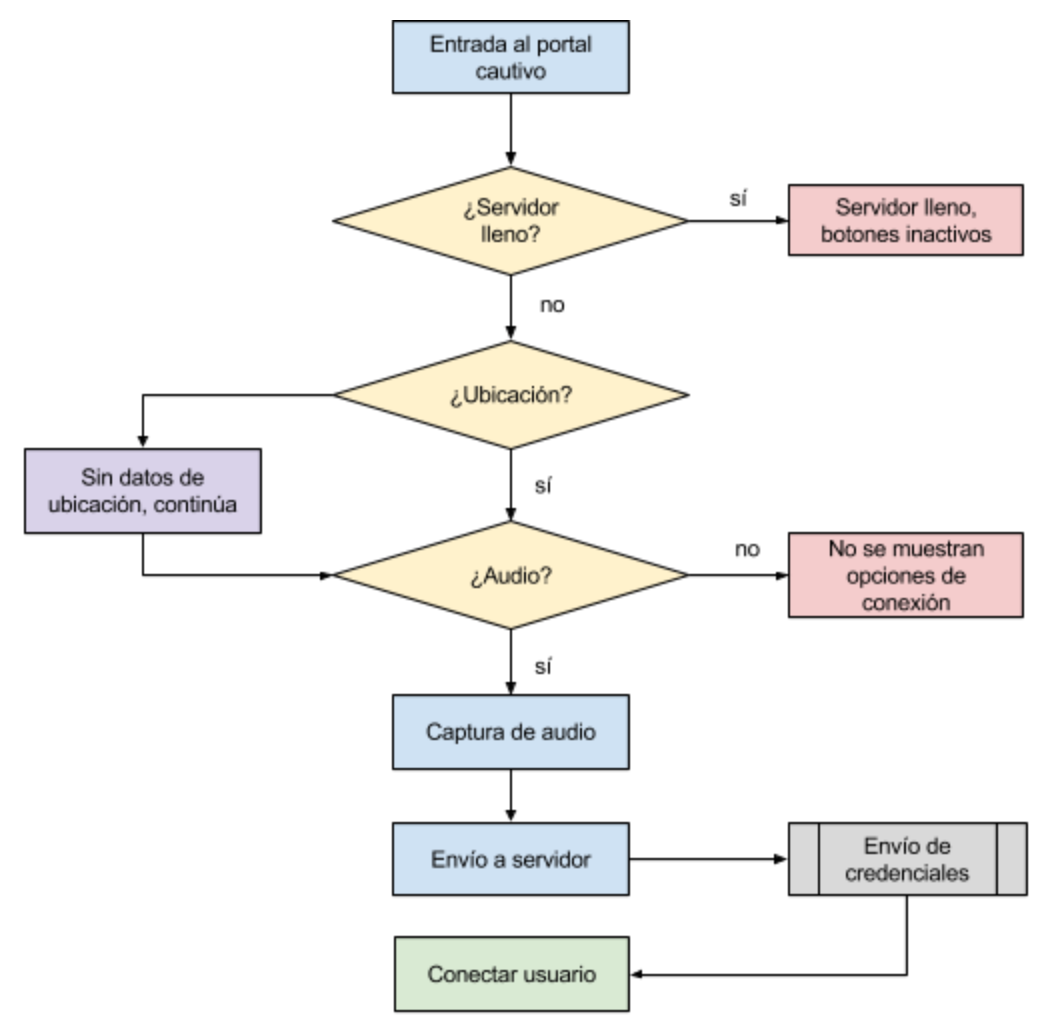
\includegraphics[width=0.75\linewidth]{./5_AnalisisOrganico/Img/flujoBotones.png}
\end{center}
\caption{Organigrama que indica cómo cambian los botones}
% \source{http://coova.github.io/CoovaChilli/}
\label{flujoBotones}
\end{figure}

Usando Bootstrap se logra un diseño responsivo. Esto es, la apariencia de la página Web mantiene unas proporciones estéticas adaptadas al tamaño del dispositivo utilizado, pudiendo utilizar cómodamente el servicio tanto desde un ordenador portátil como desde un teléfono móvil o una tablet. Se adjuntan capturas de pantalla de cómo se ve la interfaz Web en cada uno de los pasos desde un teléfono móvil (Figura \ref{responsiveDesign}).

\begin{figure}[!t]
\begin{center}
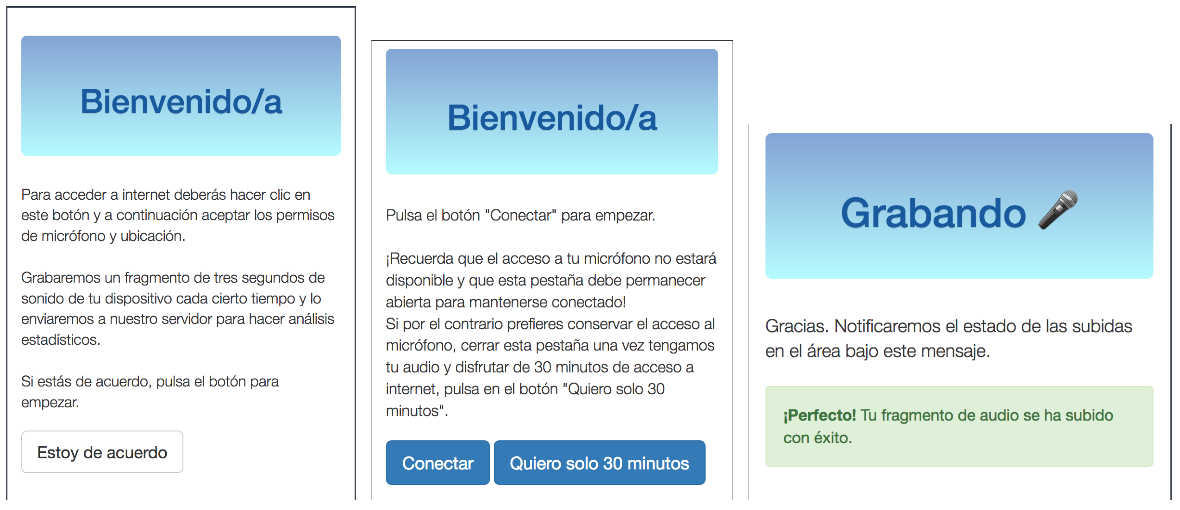
\includegraphics[width=0.75\linewidth]{./5_AnalisisOrganico/Img/responsiveDesign.png}
\end{center}
\caption{Diseño responsivo de la página Web principal}
% \source{http://coova.github.io/CoovaChilli/}
\label{responsiveDesign}
\end{figure}

El comportamiento de la aplicación Web aparte de su contenido visual vienen determinados por los \emph{scripts} incluidos en el archivo HTML justo antes de cerrar la etiqueta \emph{body}, que son analizados a continuación. Los archivos se encuentran en el directorio \emph{js} de nuestro árbol de directorios.

\begin{listing}[H]
\begin{minted}
[
frame=lines,
framesep=2mm,
baselinestretch=1.2,
bgcolor=lightgray,
fontsize=\footnotesize,
breaklines=true,
breaksymbolleft={}
]
{html}
<!DOCTYPE html>
<html lang="en">
<head>
// ...
</head>
<body>
// ...
<script src="js/jquery-3.2.1.min.js"></script>
<script src="js/bootstrap.min.js"></script>
<script src="js/ChilliLibrary.js"></script>
<script src="js/chilliController.js"></script>
<script src="js/script.js"></script>
</body>
</html>
\end{minted}
\caption{scripts importados en el documento HTML}
% \label{usersControllerImports}
\end{listing}

Los dos primeros \emph{scripts} incluidos son los \emph{frameworks} jQuery y Bootstrap, utilizados para facilitar la programación de peticiones AJAX y gestionar la interfaz de usuario, respectivamente, también se incluyó en la cabecera un archivo CSS de Bootstrap para funcionar junto al archivo JavaScript. Además, el \emph{framework} Bootstrap por sí mismo requiere de jQuery para funcionar correctamente.

El archivo \emph{ChilliLibrary.js}, como ya se adelantó en el capítulo 2, se encarga de crear un objeto global denominado \emph{chilliController} en nuestra \emph{Aplicación Web}, mediante el cual podemos comunicarnos con CoovaChilli, gestionar el inicio y cierre de sesiones y consultar la información de contabilidad.

El archivo \emph{chilliController.js} ajusta los parámetros del objeto \emph{chilliController} y aporta los métodos a ser usados por la \emph{Aplicación Web} actuando como capa intermedia entre el objeto \emph{chilliController} y el resto de elementos de la misma, como puede verse en los métodos de \emph{connect()} y \emph{disconnect()} que son llamados por el archivo \emph{script.js}.

\begin{listing}[H]
\begin{minted}
[
frame=lines,
framesep=2mm,
baselinestretch=1.2,
bgcolor=lightgray,
fontsize=\footnotesize,
breaklines=true,
breaksymbolleft={}
]
{javascript}
chilliController.ssl = true;

function connect(username, password){
    chilliController.logon(username, password);
}

function disconnect(userCreds){
   liberateUser(userCreds);
   chilliController.logoff();
}
\end{minted}
\caption{Habilitación de SSL, conexión y desconexión}
% \label{usersControllerImports}
\end{listing}

La función \emph{liberateUser()} se analiza en el apartado \ref{script.js} dedicado al archivo \emph{scripts.js}.
Además, asocia funciones locales a eventos del objeto \emph{chilliController} y se encarga de consultar el estado del mismo al ejecutarse por primera vez.

\begin{listing}[H]
\begin{minted}
[
frame=lines,
framesep=2mm,
baselinestretch=1.2,
bgcolor=lightgray,
fontsize=\footnotesize,
breaklines=true,
breaksymbolleft={}
]
{javascript}
chilliController.onError  = handleErrors;
chilliController.onUpdate = updateUI
// when the reply is ready, this handler function is called
function updateUI( cmd ) {
    console.log('You called the method ' + cmd +
        '\n Your current state is = ' + chilliController.clientState);
}
// If an error occurs, this handler will be called instead
function handleErrors ( code ) {
    console.log( 'The last contact with the Controller failed. Error code = ' + code );
}
//  finally, get current state
chilliController.refresh();
\end{minted}
\caption{Funciones adicionales de chilliController.js}
% \label{usersControllerImports}
\end{listing}

\paragraph{El archivo \emph{script.js}} \label{script.js} ~\\

La funcionalidad de la Aplicación Web viene determinada en gran medida por este archivo JavaScript, que hace uso de los siguientes variables y métodos.

\begin{listing}[H]
\begin{minted}
[
frame=lines,
framesep=2mm,
baselinestretch=1.2,
bgcolor=lightgray,
fontsize=\footnotesize,
breaklines=true,
breaksymbolleft={}
]
{javascript}
'use strict';

let id = val => document.getElementById(val),
    agreeBtn = id('agreeBtn'),
    recordBtn = id('recordBtn'),
    recordBtn30min = id('recordBtn30min'),
    alertsArea = id('alertsArea'),
    stream,
    recorder,
    chunks,
    media,
    serverStatus,
    locationTime;

var userCreds = {
    id: -1,
    username: "prueba",
    password: "pruebaPass",
    oneTimePass: false,
    connected: 0
};
\end{minted}
\caption{Funciones adicionales de chilliController.js}
% \label{usersControllerImports}
\end{listing}

La primera variable utiliza la función flecha (\emph{arrow function}) implementada en ECMAScript 6, y es equivalente a la sintaxis siguiente: \emph{let id = function(val) \{ return document.getElementById(val) \};}. Esta función es una forma abreviada de obtener los elementos del documento HTML, como puede verse en las cuatro siguientes variables: \emph{agreeBtn}, \emph{recordBtn}, \emph{recordBtn30min} y \emph{alertsArea} que corresponden a los elementos con ese identificador del documento HTML.

Las variables \emph{stream}, \emph{recorder}, \emph{chunks} y \emph{media} son utilizadas por las API WebRTC y \emph{MediaStream Recording} para su funcionalidad, que veríamos en acción al analizar los métodos del archivo. Las variables \emph{serverStatus}, \emph{locationTime} y \emph{userCreds} almacenan el estado del servidor en forma booleana, la latitud, longitud y marca de tiempo para usar en los nombres de los archivos de audio y las credenciales de usuario recibidas desde el servidor, respectivamente.

Al ser cargada la \emph{Aplicación Web} se ejecutan los siguientes métodos por medio de \emph{window.onload}.

\begin{listing}[H]
\begin{minted}
[
frame=lines,
framesep=2mm,
baselinestretch=1.2,
bgcolor=lightgray,
fontsize=\footnotesize,
breaklines=true,
breaksymbolleft={}
]
{javascript}
window.onload = () => {
    prepareSite();
    checkServerStatus();
    setInterval(checkServerStatus(), 500000);
};

function prepareSite() {
    if (navigator.geolocation) {
        try {
            navigator.geolocation.watchPosition(showPositionTime, positionError, geoOptions);
        }
        catch (err) {
            locationTime = 'LocError';
        }
    } else {
        locationTime = 'Geolocation is not supported by this browser';
    }
}

function checkServerStatus() {
    $.ajax({
        type: 'GET',
        url: '/serverstatus',
        dataType: 'text',
        success: function (data) {
            if (data === "true") {
                serverStatus = true;
            } else {
                serverStatus = false;
                agreeBtn.disabled = true;
                agreeBtn.textContent = "Servidor lleno";
            }
        }
    });
}
\end{minted}
\caption{Preparando el portal cautivo según llega el usuario}
% \label{usersControllerImports}
\end{listing}

La función \emph{prepareSite()} simplemente intenta activar la geolocalización del dispositivo a lo largo del tiempo mediante la función \emph{watchPosition()}, lo que implica que nada más cargar la página aparece la petición de permisos de ubicación, que el usuario puede aceptar o negar sin que eso perturbe el resto de la experiencia de usuario. Obviamente, si el usuario niega los permisos el servicio no contaría con los datos de ubicación de los archivos de audio procedentes de esta instancia de la Aplicación Web, pero en principio se ha diseñado teniéndolo en cuenta.

La función \emph{watchPosition()} cuenta con dos funciones \emph{callback} (en orden, manejadores de éxito y error) como dos primeros parámetros y un tercer parámetro de opciones, que en este caso simplemente activa la alta precisión de los datos entregados a la aplicación Web. Aquí se ven las implantaciones de estos tres parámetros.

\begin{listing}[H]
\begin{minted}
[
frame=lines,
framesep=2mm,
baselinestretch=1.2,
bgcolor=lightgray,
fontsize=\footnotesize,
breaklines=true,
breaksymbolleft={}
]
{javascript}
function showPositionTime(position) {
    locationTime = 'Lat' + position.coords.latitude +
        'Lon' + position.coords.longitude +
        'Time' + new Date();
}

var geoOptions = {
    enableHighAccuracy: true
};

function positionError(positionError) {
    console.log('Error ' + positionError.code + ' in geolocation: ' + positionError.message);
}
\end{minted}
\caption{Funciones y opciones para geolocalización}
% \label{usersControllerImports}
\end{listing}

Como puede verse, la función llamada al tener éxito en la solicitud de permisos de ubicación es la que almacena en la variable \emph{locationTime} los datos de ubicación y marca de tiempo, tal y como comentábamos al principio de la sección dedicada a este archivo.

La función \emph{checkServerStatus()} cuenta con la primera petición AJAX (de tipo GET a la ruta \emph{/serverstatus} que ya analizamos en la sección del servidor) realizada por el sistema. Aquí la \emph{Aplicación Web} insta al servidor a que compruebe su estado, buscando si hay usuarios libres para que la instancia de la aplicación pueda unir al usuario al servicio. Se establece también un intervalo de tiempo pasado el cual se vuelve a consultar el estado del servidor.

También se implanta un manejador de eventos para desconectar al usuario en caso de que cierre la pestaña del portal cautivo, lo que logra el requisito de que el usuario tenga que tener una pestaña del navegador abierta con la instancia de la \emph{Aplicación Web} en todo momento para no perder la conexión.

\begin{listing}[H]
\begin{minted}
[
frame=lines,
framesep=2mm,
baselinestretch=1.2,
bgcolor=lightgray,
fontsize=\footnotesize,
breaklines=true,
breaksymbolleft={}
]
{javascript}
window.onbeforeunload = e => {
    if (userCreds.id >= 0 && userCreds.oneTimePass == false) {
        disconnect(userCreds);
        userCreds.id = -1;
    }
    var dialogText = "Disconnecting...";
    e.returnValue = dialogText;
    return dialogText;
};
\end{minted}
\caption{Desconectando al usuario que abandona la página}
% \label{usersControllerImports}
\end{listing}

Este manejador llama a la función \emph{disconnect()} del objeto \emph{chilliController}, que a su vez llama a \emph{liberateUser()}, ambas con el identificador de usuario actual como parámetro en caso de que estuviera conectado. La función \emph{liberateUser()} no es más que otra petición AJAX al servidor con la ruta \emph{/userlogoff}, instándole a marcar el usuario como inactivo en la base de datos.

\begin{listing}[H]
\begin{minted}
[
frame=lines,
framesep=2mm,
baselinestretch=1.2,
bgcolor=lightgray,
fontsize=\footnotesize,
breaklines=true,
breaksymbolleft={}
]
{javascript}
function liberateUser(creds) {
    $.ajax({
        type: 'POST',
        url: '/userlogoff',
        data: creds,
        success: function (data) {
            console.log('success ' + data);
        }
    });
}
\end{minted}
\caption{Marcando usuario como desconectado en el servidor node}
% \label{usersControllerImports}
\end{listing}

Después de esto se programan los comportamientos de los botones. El primer botón que aparece en la visualización de la página es el que se debe pulsar al estar de acuerdo con las condiciones que se expresan en la primera descripción, teniendo este el identificador \emph{agreeBtn}. Este botón intenta configurar la captura de audio en el dispositivo según las API WebRTC y \emph{MediaStream Recording}, configurando las opciones de la grabación (en nuestro caso declarando que se captura audio, utilizando el \emph{\acrshort{MIME} type} y la extensión de archivo correspondiente al formato \emph{Ogg} \cite{OggRFC1, OggRFC2}) y determinando qué hacer con los archivos de audio generados según el tipo de usuario o si este tiene credenciales ya asignadas. Si el usuario deniega permisos o el dispositivo no soporta la tecnología utilizada el botón se desactiva y es imposible seguir adelante.

\begin{listing}[H]
\begin{minted}
[
frame=lines,
framesep=2mm,
baselinestretch=1.2,
bgcolor=lightgray,
fontsize=\footnotesize,
breaklines=true,
breaksymbolleft={}
]
{javascript}
agreeBtn.onclick = e => {
    let mediaOptions = {
        audio: {
            tag: 'audio',
            type: 'audio/ogg',
            ext: '.ogg',
            gUM: { audio: true }
        }
    };

    media = mediaOptions.audio;
    navigator.mediaDevices.getUserMedia(media.gUM).then(_stream => {
        stream = _stream;
        id('gUMArea').style.display = 'none';
        id('preRecordArea').style.display = 'inherit';
        recorder = new MediaRecorder(stream);
        recorder.ondataavailable = e => {
            chunks.push(e.data);
            if (recorder.state == 'inactive') {
                if (userCreds.id >= 0) {
                    loggedUserSaveAndSend();
                } else if (userCreds.oneTimePass === false) {
                    saveAndSend();
                } else {
                    saveAndSendOneTimePass();
                }
            }
        };
        log('got media successfully');
    }).catch(function(err){
        agreeBtn.disabled = true;
        agreeBtn.textContent = "Permiso denegado o incompatible";
    });
};
\end{minted}
\caption{Preparación para grabar y enviar el fragmento de audio}
% \label{usersControllerImports}
\end{listing}

Lo que activa el evento \emph{ondataavailable} es la finalización de una grabación de audio. Para controlar el inicio y final de estas grabaciones, así como su periodicidad, se utiliza una función que controla al segundo botón de la interfaz de usuario, que tiene el identificador \emph{recordBtn}, así como las sencillas funciones de inicio y parada implementadas según la API \emph{MediaStream Recording}. En caso de que el usuario seleccione la opción de conectarse durante 30 minutos habría pulsado el botón con el identificador \emph{recordBtn30min}, que tiene una estructura muy similar, solo variando en que no hay un intervalo regular donde la  grabación vuelva a empezar.

\begin{listing}[H]
\begin{minted}
[
frame=lines,
framesep=2mm,
baselinestretch=1.2,
bgcolor=lightgray,
fontsize=\footnotesize,
breaklines=true,
breaksymbolleft={}
]
{javascript}
recordBtn.onclick = e => {
    if (serverStatus === true) {
        userCreds.oneTimePass = false;
        id('preRecordArea').style.display = 'none';
        id('agreedArea').style.display = 'inherit';
        setTimeout(startRecording, 100);
        setInterval(startRecording, 180000);
    } else {
        console.log('Error');
    }
};

recordBtn30min.onclick = e => {
    if (serverStatus === true) {
        userCreds.oneTimePass = true;
        id('preRecordArea').style.display = 'none';
        id('agreedArea').style.display = 'inherit';
        setTimeout(startRecording, 100);
    } else {
        console.log('Error');
    }
};

function startRecording() {
    chunks = [];
    recorder.start();
    setTimeout(stopRecording, 5000);
}

function stopRecording() {
    recorder.stop();
}
\end{minted}
\caption{Grabando al ser autorizado por el usuario}
% \label{usersControllerImports}
\end{listing}

Como también puede verse en el último condicional de la función \emph{agreeBtn.onclick}, la anterior al último bloque de código, la función que se llamaría al final de cada grabación depende de si el usuario del servicio tiene unas credenciales asignadas o no en la variable \emph{userCreds} de su instancia de la aplicación Web o si, por el contrario, solo optó por conectarse durante 30 minutos. Estas tres funciones son muy similares en cuanto a que preparan el archivo para su envío al servidor mediante AJAX y lo renombran según los datos de ubicación y tiempo obtenidos y las opciones de audio, pero las rutas son diferentes y solo se intenta obtener credenciales en el caso de que no existan ya unas asignadas.

\begin{listing}[H]
\begin{minted}
[
frame=lines,
framesep=2mm,
baselinestretch=1.2,
bgcolor=lightgray,
fontsize=\footnotesize,
breaklines=true,
breaksymbolleft={}
]
{javascript}
function saveAndSend() {
    let blob = new Blob(chunks, { type: media.type });
    var fd = new FormData();
    fd.append('blob', blob, `${locationTime}${media.ext}`);

    $.ajax({
        url: '/upload',
        type: 'POST',
        data: fd,
        processData: false,
        contentType: false,
        success: function (data) {
            console.log('[Normal] upload successful! ' + data);
            receiveResponse();
            setAlert("success");
        },
        error: function (data) {
            console.log('[Normal] upload error ' + data);
            setAlert("error");
        }
    });
}
\end{minted}
\caption{Guardando y enviando el fragmento de audio (usuario recién llegado)}
% \label{usersControllerImports}
\end{listing}

\begin{listing}[H]
\begin{minted}
[
frame=lines,
framesep=2mm,
baselinestretch=1.2,
bgcolor=lightgray,
fontsize=\footnotesize,
breaklines=true,
breaksymbolleft={}
]
{javascript}
function loggedUserSaveAndSend() {
    let blob = new Blob(chunks, { type: media.type });
    var fd = new FormData();
    fd.append('blob', blob, `${locationTime}${media.ext}`);

    $.ajax({
        url: '/loggedupload',
        type: 'POST',
        data: fd,
        processData: false,
        contentType: false,
        success: function (data) {
            console.log('[Logged] upload successful! ' + data);
            setAlert("success");
        },
        error: function (data) {
            console.log('[Logged] upload error ' + data);
            setAlert("errorLogged");
        }
    });
}
\end{minted}
\caption{Guardando y enviando el fragmento de audio (usuario ya conectado)}
% \label{usersControllerImports}
\end{listing}

\begin{listing}[H]
\begin{minted}
[
frame=lines,
framesep=2mm,
baselinestretch=1.2,
bgcolor=lightgray,
fontsize=\footnotesize,
breaklines=true,
breaksymbolleft={}
]
{javascript}
function saveAndSendOneTimePass() {
    let blob = new Blob(chunks, { type: media.type });
    var fd = new FormData();
    fd.append('blob', blob, `${locationTime}${media.ext}`);

    $.ajax({
        url: '/onetimepassupload',
        type: 'POST',
        data: fd,
        processData: false,
        contentType: false,
        success: function (data) {
            console.log('[One-time] upload successful! ' + data);
            receiveResponse();
            setAlert("successOneTime");
        },
        error: function (data) {
            console.log('[One-time] upload error ' + data);
            setAlert("error");
        }
    });
}
\end{minted}
\caption{Guardando y enviando el fragmento de audio (usuario de 30 minutos)}
% \label{usersControllerImports}
\end{listing}

Nótese que en la segunda función, \emph{loggedUserSaveAndSend()}, aparte de variar la ruta, no se llama a la función \emph{receiveResponse()} al finalizar la transacción con éxito. En el caso de la primera función, el servidor habría guardado en su variable \emph{creds} las credenciales a utilizar, por lo que la \emph{Aplicación Web} realiza otra petición AJAX para obtenerlas.

\begin{listing}[H]
\begin{minted}
[
frame=lines,
framesep=2mm,
baselinestretch=1.2,
bgcolor=lightgray,
fontsize=\footnotesize,
breaklines=true,
breaksymbolleft={}
]
{javascript}
function receiveResponse() {
    $.ajax({
        type: 'GET',
        url: '/creds',
        dataType: 'json',
        success: function (data) {
            userCreds = data;
            connectUser(userCreds);
        }
    });
}
\end{minted}
\caption{Recibiendo credenciales del servidor}
% \label{usersControllerImports}
\end{listing}

Al tener éxito en esta petición las credenciales quedan almacenadas en la variable local \emph{userCreds}, por lo que solo queda conectarse con ellas por medio la función \emph{connect()} del objeto \emph{chilliController}, esperar un tiempo para que se realice la conexión y notificar al servidor del resultado del intento.

\begin{listing}[H]
\begin{minted}
[
frame=lines,
framesep=2mm,
baselinestretch=1.2,
bgcolor=lightgray,
fontsize=\footnotesize,
breaklines=true,
breaksymbolleft={}
]
{javascript}
function connectUser(data) {
    connect(data.username, data.password);

    setTimeout(2500, function () {
        if (chilliController.clientState === 1) {
            userCreds.connected = chilliController.clientState;
            $.ajax({
                type: 'POST',
                url: '/userconnected',
                data: userCreds,
                success: function (data) {
                    console.log('success ' + data);
                }
            });
        } else if (chilliController.clientState === 2) {
            setAlert("error");
        }
    });
}
\end{minted}
\caption{Intentando la conexión y comprobando el resultado}
% \label{usersControllerImports}
\end{listing}

Por último, la \emph{Aplicación Web} tiene un campo de alertas que notifican al usuario de la recepción de archivos de audio o errores durante las mismas mediante la función \emph{setAlert()}, llamada por otras funciones de este archivo ya expuestas anteriormente.

\begin{listing}[H]
\begin{minted}
[
frame=lines,
framesep=2mm,
baselinestretch=1.2,
bgcolor=lightgray,
fontsize=\footnotesize,
breaklines=true,
breaksymbolleft={}
]
{javascript}
function setAlert(info) {
    var newDiv = document.createElement("div");
    switch (info) {
        case "success":
            newDiv.className = "alert alert-success";
            newDiv.role = "alert";
            newDiv.innerHTML = "<strong>¡Perfecto!</strong> Tu fragmento de audio se ha subido con éxito.";
            break;
        case "error":
            newDiv.className = "alert alert-danger";
            newDiv.role = "alert";
            newDiv.innerHTML = "<strong>¡Vaya!</strong> Ha habido un error... Aún no tienes internet. <strong>Trata de conectarte de nuevo.</strong>";
            break;
        case "errorLogged":
            newDiv.className = "alert alert-danger";
            newDiv.role = "alert";
            newDiv.innerHTML = "<strong>¡Vaya!</strong> Ha habido un error enviando el fichero... Volveremos a intentarlo más tarde.";
            break;
        case "successOneTime":
            newDiv.className = "alert alert-success";
            newDiv.role = "alert";
            newDiv.innerHTML = "<strong>¡Perfecto!</strong> Tu fragmento de audio se ha subido con éxito. <strong>Ya puedes cerrar esta pestaña en tu navegador y disfrutar de tus 30 minutos de internet.</strong>";
            break;
    }
    alertsArea.appendChild(newDiv);
}
\end{minted}
\caption{Sistema de alertas para informar al usuario}
% \label{usersControllerImports}
\end{listing}
\cleardoublepage
\clearpage
\vspace*{\stretch{2}}%{\fill}
\begin{center}
\begin{minipage}{.75\textwidth}
\section{Análisis de la evaluación empírica}

Presentados la instalación del \emph{hardware} necesario y el análisis orgánico del software usado y programado desde cero, subrayar que por las características mínimas de la interfaz de usuario no es necesario dedicar más análisis que el realizado hasta el momento. En este capítulo presentamos los resultados experimentales de la evaluación del sistema con distintos tipos de terminales móviles. % \pagebreak
\end{minipage}
\end{center}
\vspace{\stretch{3}} % \vfill % equivalent to \vspace{\fill}
\clearpage% https://tex.stackexchange.com/questions/70714/center-horizontally-and-vertically-a-block-of-text

\subsection{Resultados con una tableta Android}
A continuación se muestra cómo un dispositivo portátil (en este caso una \emph{tablet} Samsung Galaxy GP-P5210, de 1 GB de RAM y con el sistema operativo Android 4.4.2) puede enviar su audio, recibir las credenciales en respuesta y conectarse a Internet. Las pruebas se hicieron con el navegador Chrome 61 y se monitorizaron los procesos con las herramientas de depuración remota de \emph{Chrome DevTools} \cite{ChromeDevTools}.
 
En la Figura \ref{connectionChilli} se muestran resaltados los datos relevantes en el proceso de conexión exitoso, en orden descendiente, correspondientes al guardado y envío de audio, recepción de credenciales y conexión con éxito, como revela el código de estado 1 al llamar a la función \emph{logon()}.

\begin{figure}[!t]
\begin{center}
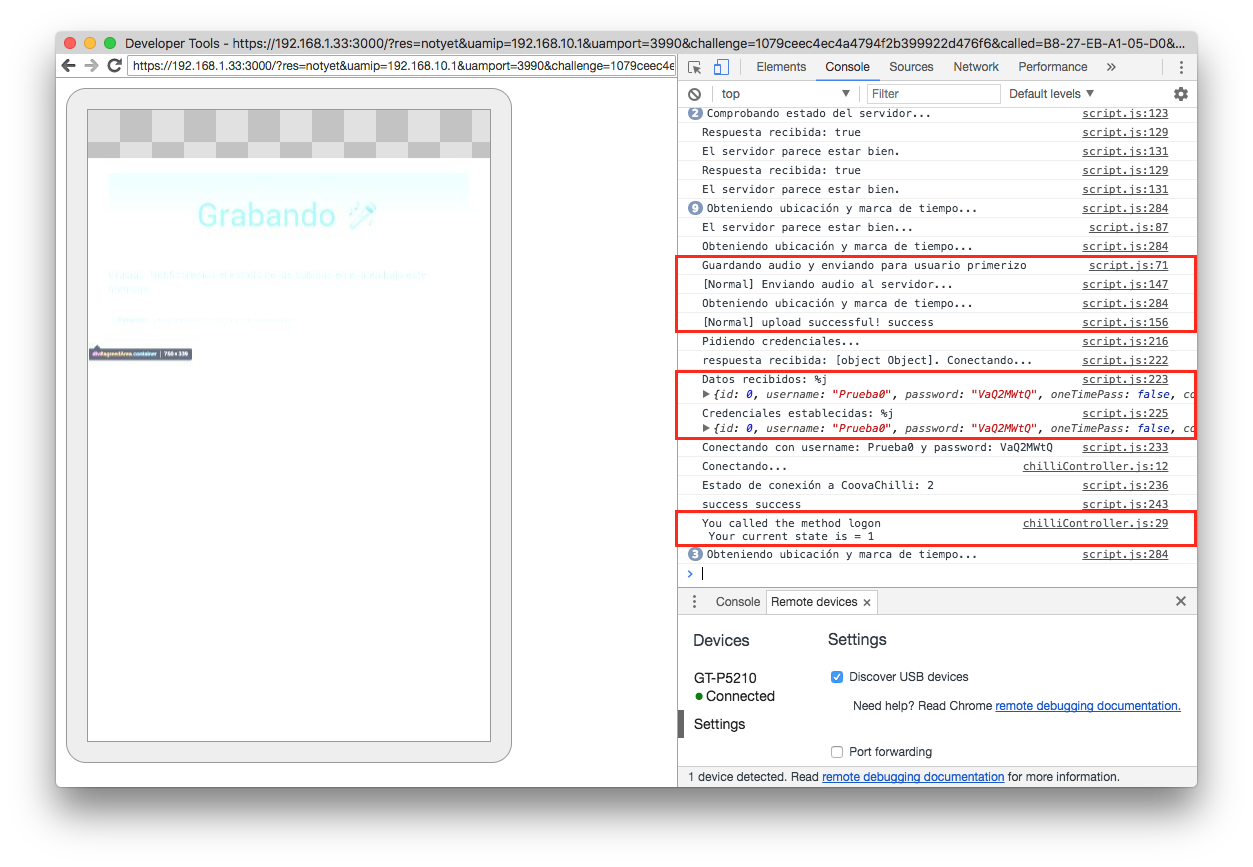
\includegraphics[width=0.75\linewidth]{./6_EvalEmpirica/Img/connectionChilli.png}
\end{center}
\caption{Datos relevantes del proceso de conexión con éxito de una tableta Android.}
\label{connectionChilli}
\end{figure}

Como se puede apreciar, cuando se envía el fichero de audio generado al servidor este responde con un objeto JavaScript que contiene las credenciales del tipo de usuario seleccionado. Tras recibir estos datos, el sistema realiza el \emph{login} con dichas credenciales, conectando al usuario a internet (como puede verse en el código de estado de la conexión, que es 1).

Dado que el proceso de desconexión automática implica cerrar la pestaña, lo que cancelaría la sesión de depuración en curso, se realizó una desconexión manual llamando a la función \emph{logoff()}. En la captura puede verse por orden descendiente el estado actual de la conexión a Internet tras llamar a la función \emph{refresh()} y la llamada a la función de desconexión y el código de estado resultante a estar desconectado (Figura \ref{chilliDisconnect}).

\begin{figure}[!t]
\begin{center}
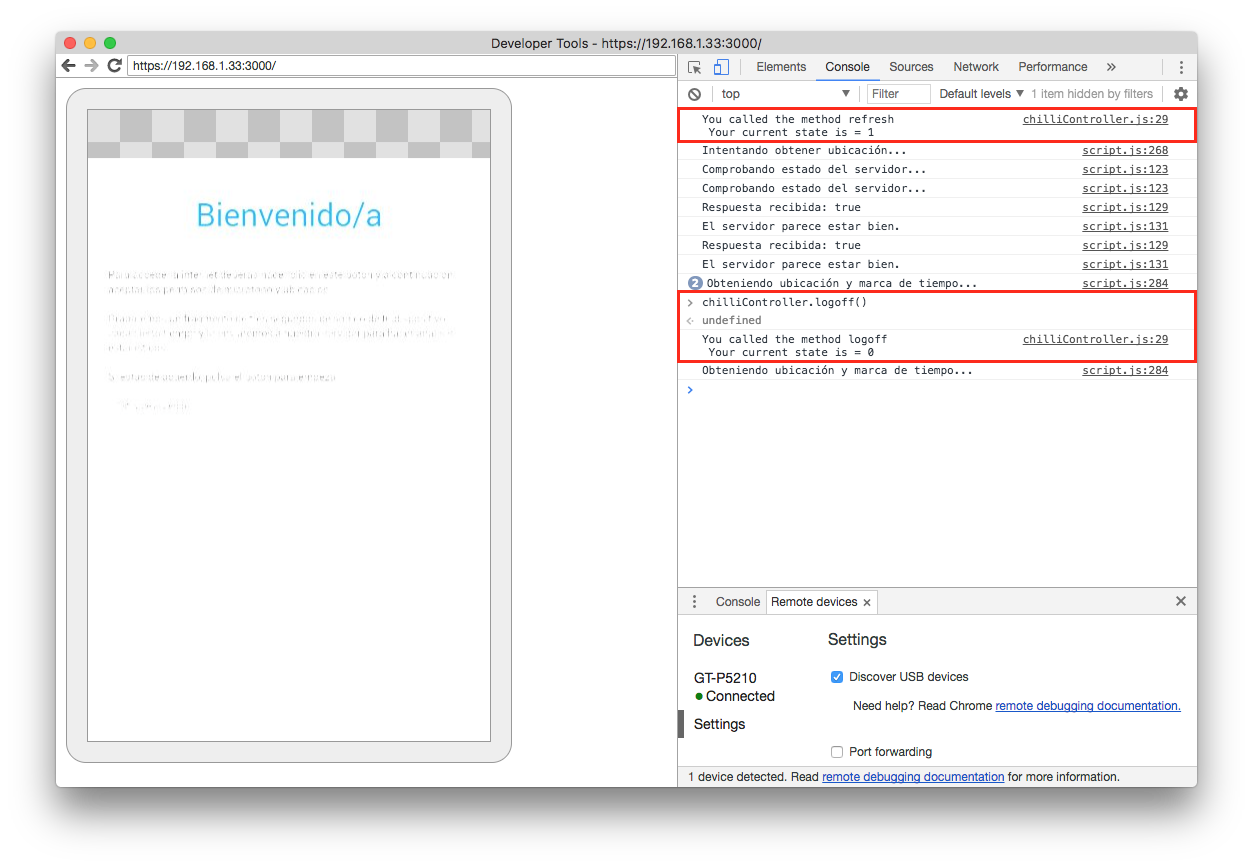
\includegraphics[width=0.75\linewidth]{./6_EvalEmpirica/Img/chilliDisconnect.png}
\end{center}
\caption{Proceso de desconexión.}
\label{chilliDisconnect}
\end{figure}

\subsection{Consumo de RAM del sistema en la Raspberry Pi}

Tras realizar las pruebas de funcionamiento pertinentes se analizó el consumo total de memoria de los procesos implicados en la implantación del sistema. Utilizando la herramienta \emph{htop}, disponible en sistemas Linux y que monitoriza la memoria física, memoria virtual, memoria de intercambio \emph{swap} y consumo de CPU tanto en valor absoluto como en porcentajes entre otras muchas cosas, se monitorizaron las estadísticas concernientes a las instancias de Node.js, \emph{hostapd}, \emph{CoovaChilli} y la estructura en la que se apoya: \emph{freeRADIUS} y \emph{MySQL}.

En la Figura \ref{htopGeneric} se muestra la ventana genérica al ejecutar el comando \verb+htop+ desde el terminal.

\begin{figure}[!t]
\begin{center}
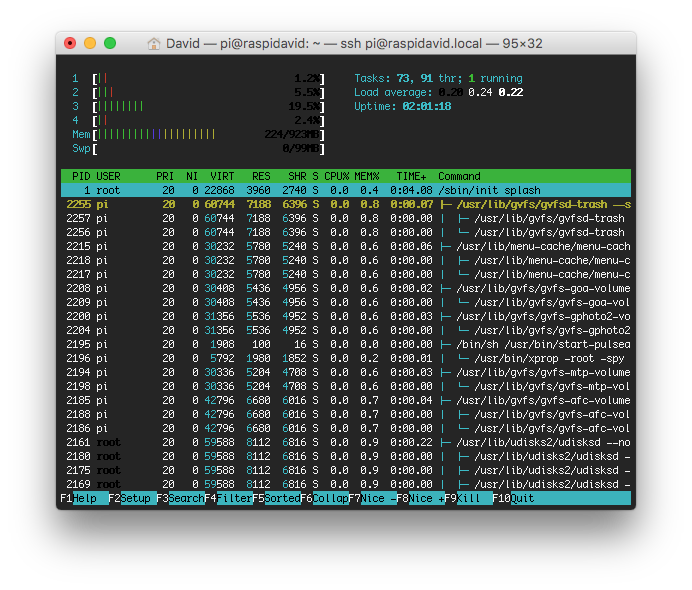
\includegraphics[width=0.75\linewidth]{./6_EvalEmpirica/Img/htopGeneric.png}
\end{center}
\caption{Ventana genérica para la orden htop.}
\label{htopGeneric}
\end{figure}

En la Figura \ref{htopNode} se muestra el consumo de recursos de Node.js.

\begin{figure}[!t]
\begin{center}
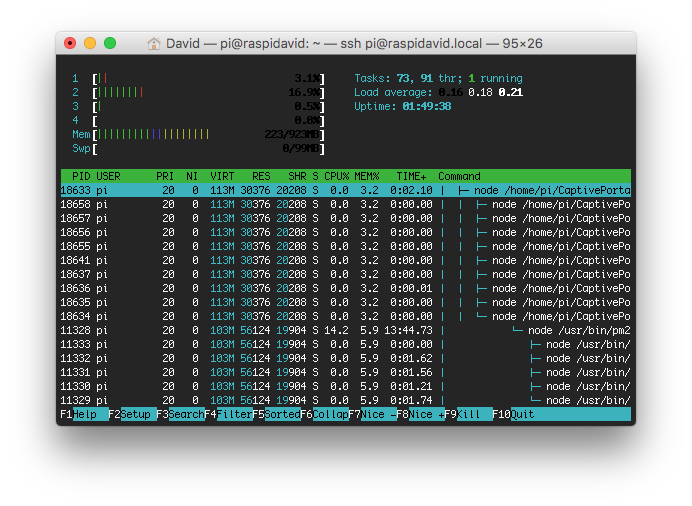
\includegraphics[width=0.75\linewidth]{./6_EvalEmpirica/Img/htopNode.png}
\end{center}
\caption{Consumo de recursos de Node.js.}
\label{htopNode}
\end{figure}

En esta captura puede apreciarse cómo el proceso que controla la instancia de la utilidad PM2 (que a su vez es la que controla la ejecución de nuestra instancia de \emph{node}) es la que destaca en el uso de recursos, utilizando un porcentaje de memoria del 5.9\% y un 14.2\% de la CPU. Lo que supone un bajo consumo.

En la Figura \ref{pm2monitNode} se muestra una cifra más inmediata del consumo total de nuestro proceso con la propia utilidad PM2, resaltada en azul en el campo superior izquierdo del monitor llamado con el comando \verb+pm2 monit+ (que se explica en el Anexo C). Que también se observa que es muy reducido.

\begin{figure}[!t]
\begin{center}
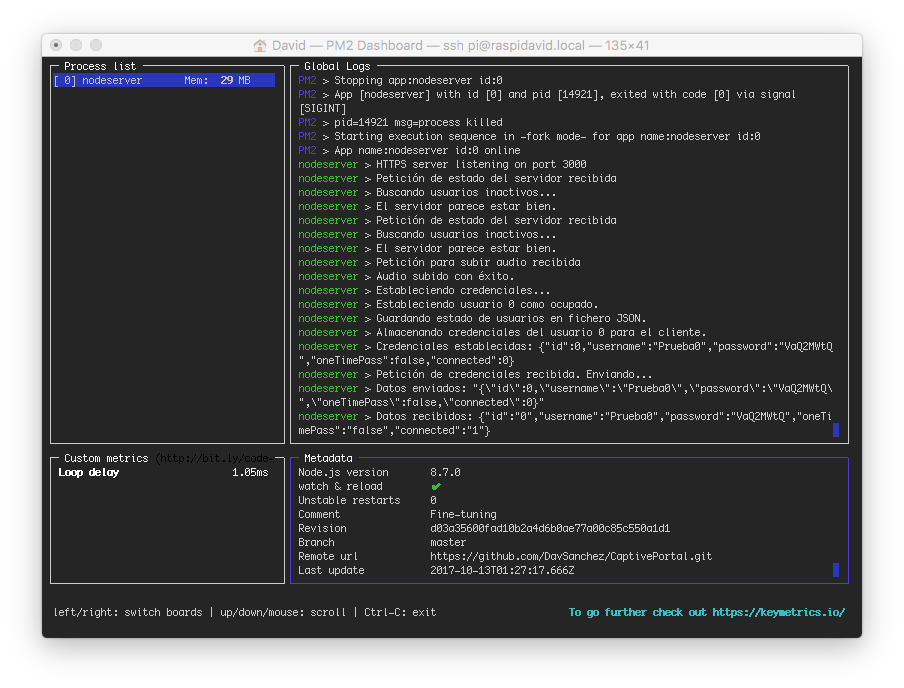
\includegraphics[width=0.75\linewidth]{./6_EvalEmpirica/Img/pm2monitNode.png}
\end{center}
\caption{Ventana de consumo usando la orden pms monit.}
\label{pm2monitNode}
\end{figure}

En la Figura \ref{htopChilli} se muestra el consumo de recursos de CoovaChilli. Se puede observar que el proceso correspondiente a CoovaChilli es ligero, no ocupando apenas procesador y un porcentaje muy bajo de la memoria total de la Raspberry Pi.

\begin{figure}[!t]
\begin{center}
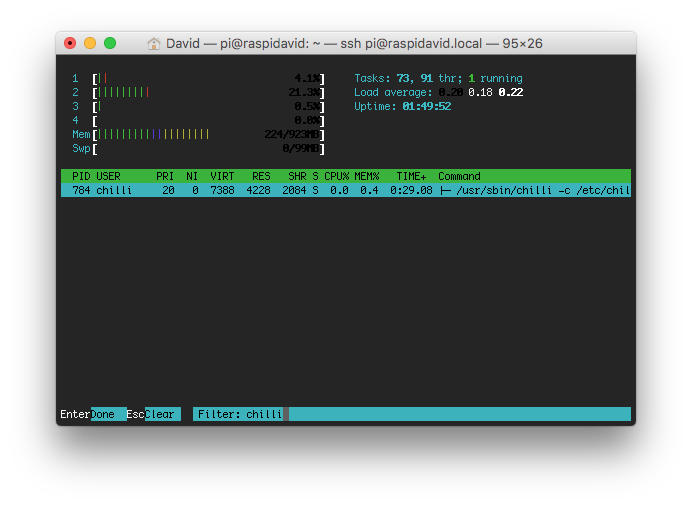
\includegraphics[width=0.75\linewidth]{./6_EvalEmpirica/Img/htopChilli.png}
\end{center}
\caption{Consumo de procesador y memoria de CoovaChilli.}
\label{htopChilli}
\end{figure}

En la Figura \ref{htopRADIUS} se muestra el consumo de recursos de freeRADIUS. Se puede observar que consume poco procesador, aunque su consumo en memoria es varias veces mayor al de CoovaChilli.

\begin{figure}[!t]
\begin{center}
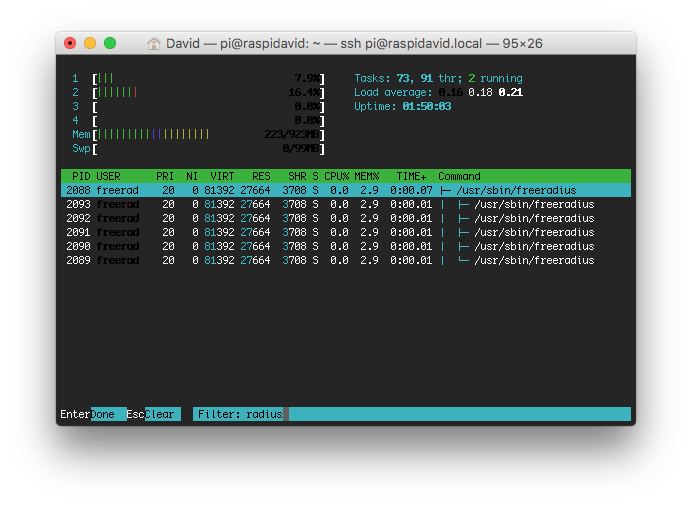
\includegraphics[width=0.75\linewidth]{./6_EvalEmpirica/Img/htopRADIUS.png}
\end{center}
\caption{Consumo de procesador y memoria de freeRADIUS.}
\label{htopRADIUS}
\end{figure}

En la Figura \ref{htopMySQL} se muestra el consumo de recursos de MySQL. Tal y como sucede con freeRADIUS, el consumo de procesador es muy bajo aunque su consumo de memoria es de hasta diez veces mayor al de CoovaChilli. Lo cual es lógico porque CoovaChilli requiere únicamente el almacenamiento de muy pocos datos relativos a conversiones de direcciones IP, en cambio ya únicamente el motor de la MySQL requiere de mucha más memoria.

\begin{figure}[!t]
\begin{center}
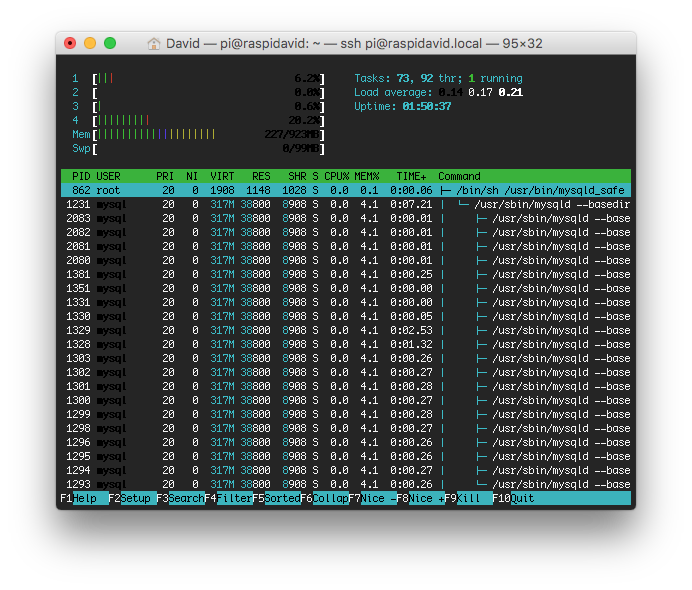
\includegraphics[width=0.75\linewidth]{./6_EvalEmpirica/Img/htopMySQL.png}
\end{center}
\caption{Consumo de procesador y memoria de MySQL.}
\label{htopMySQL}
\end{figure}

Por último, en la Figura \ref{htopHostapd} mostramos los recursos utilizados por \emph{hostapd}, cuyas estadísticas de consumo son similares al proceso de CoovaChilli.

\begin{figure}[!t]
\begin{center}
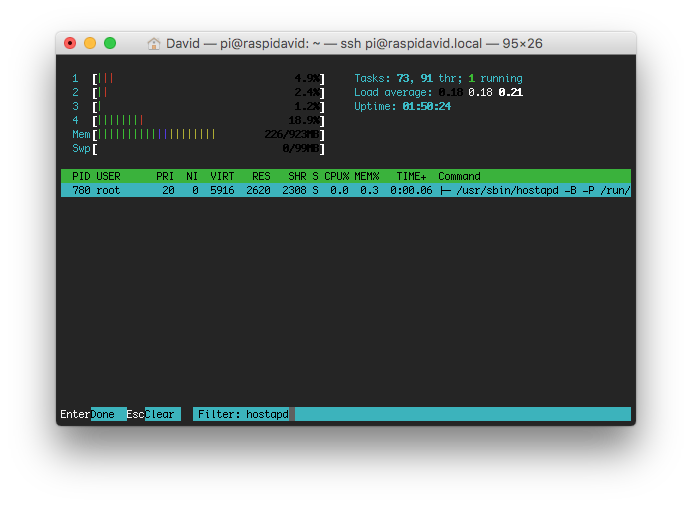
\includegraphics[width=0.75\linewidth]{./6_EvalEmpirica/Img/htopHostapd.png}
\end{center}
\caption{Consumo de procesador y memoria de Hostapd.}
\label{htopHostapd}
\end{figure}

Con estos datos podemos considerar que el sistema implementado consume aproximadamente el 15\% de los recursos del procesador y memoria RAM de la Raspberry Pi 3. Sin embargo, hay que tener en cuenta que, aparte de un ligero sobredimensionamiento de los porcentajes, muchos procesos no se dedican exclusivamente al mantenimiento de nuestro sistema, pudiendo estar consumiendo las cantidades de recursos mostradas aquí debido a que también se dedican a otras funciones (como puede ser el caso de las múltiples instancias de los procesos de MySQL).


\subsection{Consumo de RAM de los navegadores Web}

Aparte del consumo de recursos del servidor, también se estudió el consumo de recursos del sistema con el que los clientes se conectan a nuestro servicio, que en este caso no es otra cosa que el navegador Web.

En la Figura \ref{tabletChrome} se muestra una captura de ventana de uno de los dispositivos móviles utilizados, una tablet Samsung Galaxy GP-P5210, de 1 GB de RAM, con Android 4.4.2 y el navegador Chrome 61.

\begin{figure}[!t]
\begin{center}
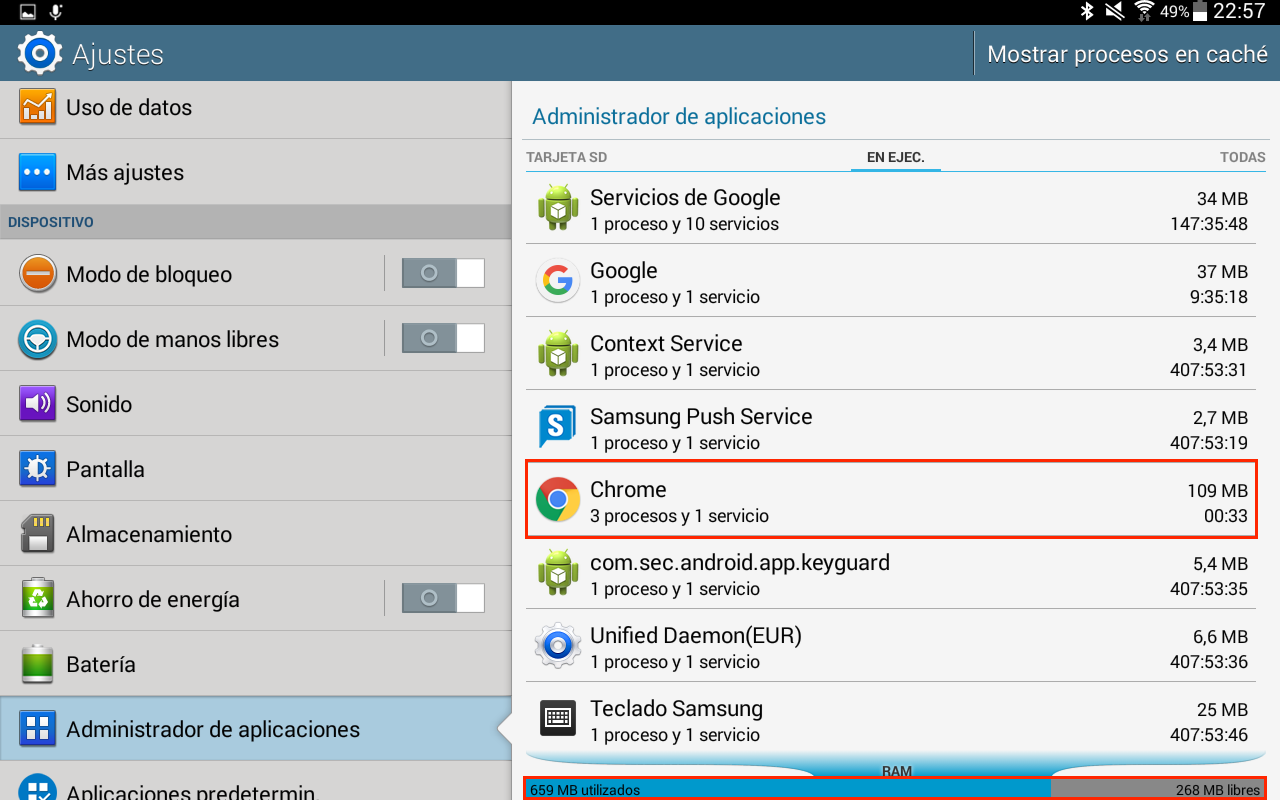
\includegraphics[width=0.75\linewidth]{./6_EvalEmpirica/Img/tabletChrome.png}
\end{center}
\caption{Ventana de consumo de RAM de los navegadores Web en una tablet Android.}
\label{tabletChrome}
\end{figure}

En las pruebas de escritorio se ha analizado el consumo de los navegadores Mozilla Firefox 57 y Vivaldi 1.12 en un equipo con macOS 10.12.6, de 16 GB de RAM, y Microsoft Edge en un equipo con Windows 10 con 8 GB. En la Figura \ref{firefoxRAM} se muestra el consumo de RAM en Mozilla Firefox para MacOS, resaltado en azul. El consumo de RAM de esta versión de Firefox puede parecer elevado sobre todo si lo comparamos con el consumo en la tablet, ya que incluso el consumo sin ningún contenido abierto y en una red diferente es tan solo entre 25 y 75 MB menor. Esto se debe en parte a las extensiones específicas y herramientas de desarrollador que vienen instaladas por defecto en esta versión.

\begin{figure}[!t]
\begin{center}
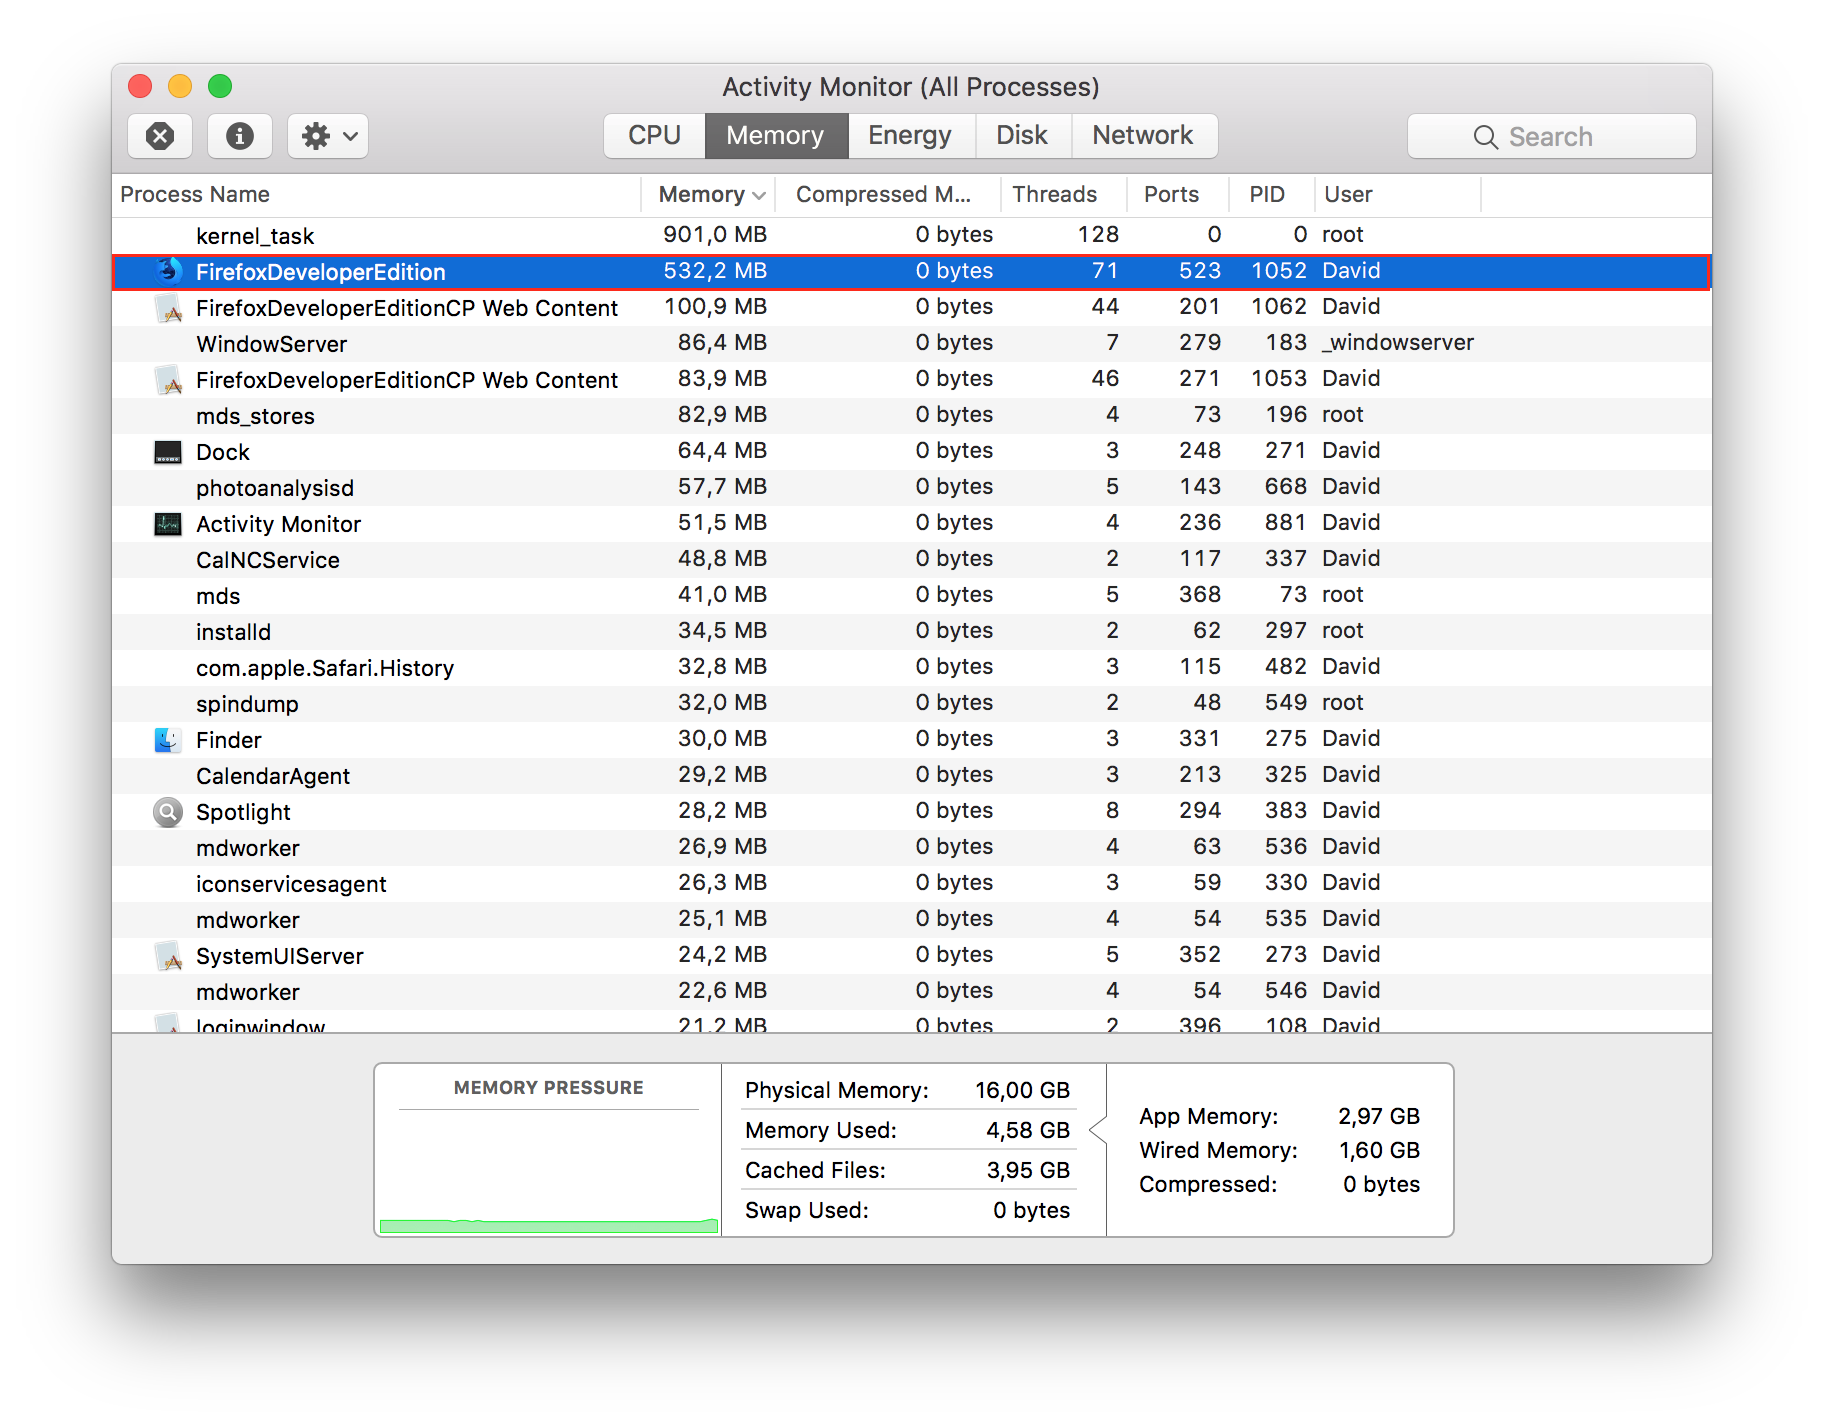
\includegraphics[width=0.75\linewidth]{./6_EvalEmpirica/Img/firefoxRAM.png}
\end{center}
\caption{Consumo de RAM de Mozilla Firefox para un computador MacOS.}
\label{firefoxRAM}
\end{figure}

El consumo de recursos en Vivaldi sin extensiones ni complementos se mantiene en unas cifras inferiores sin tener en cuenta la presencia de los Vivaldi Helpers, aunque en total el consumo sigue siendo inferior a Firefox en escritorio y superior a Chrome en Android (Figura \ref{vivaldiRAM}).

\begin{figure}[!t]
\begin{center}
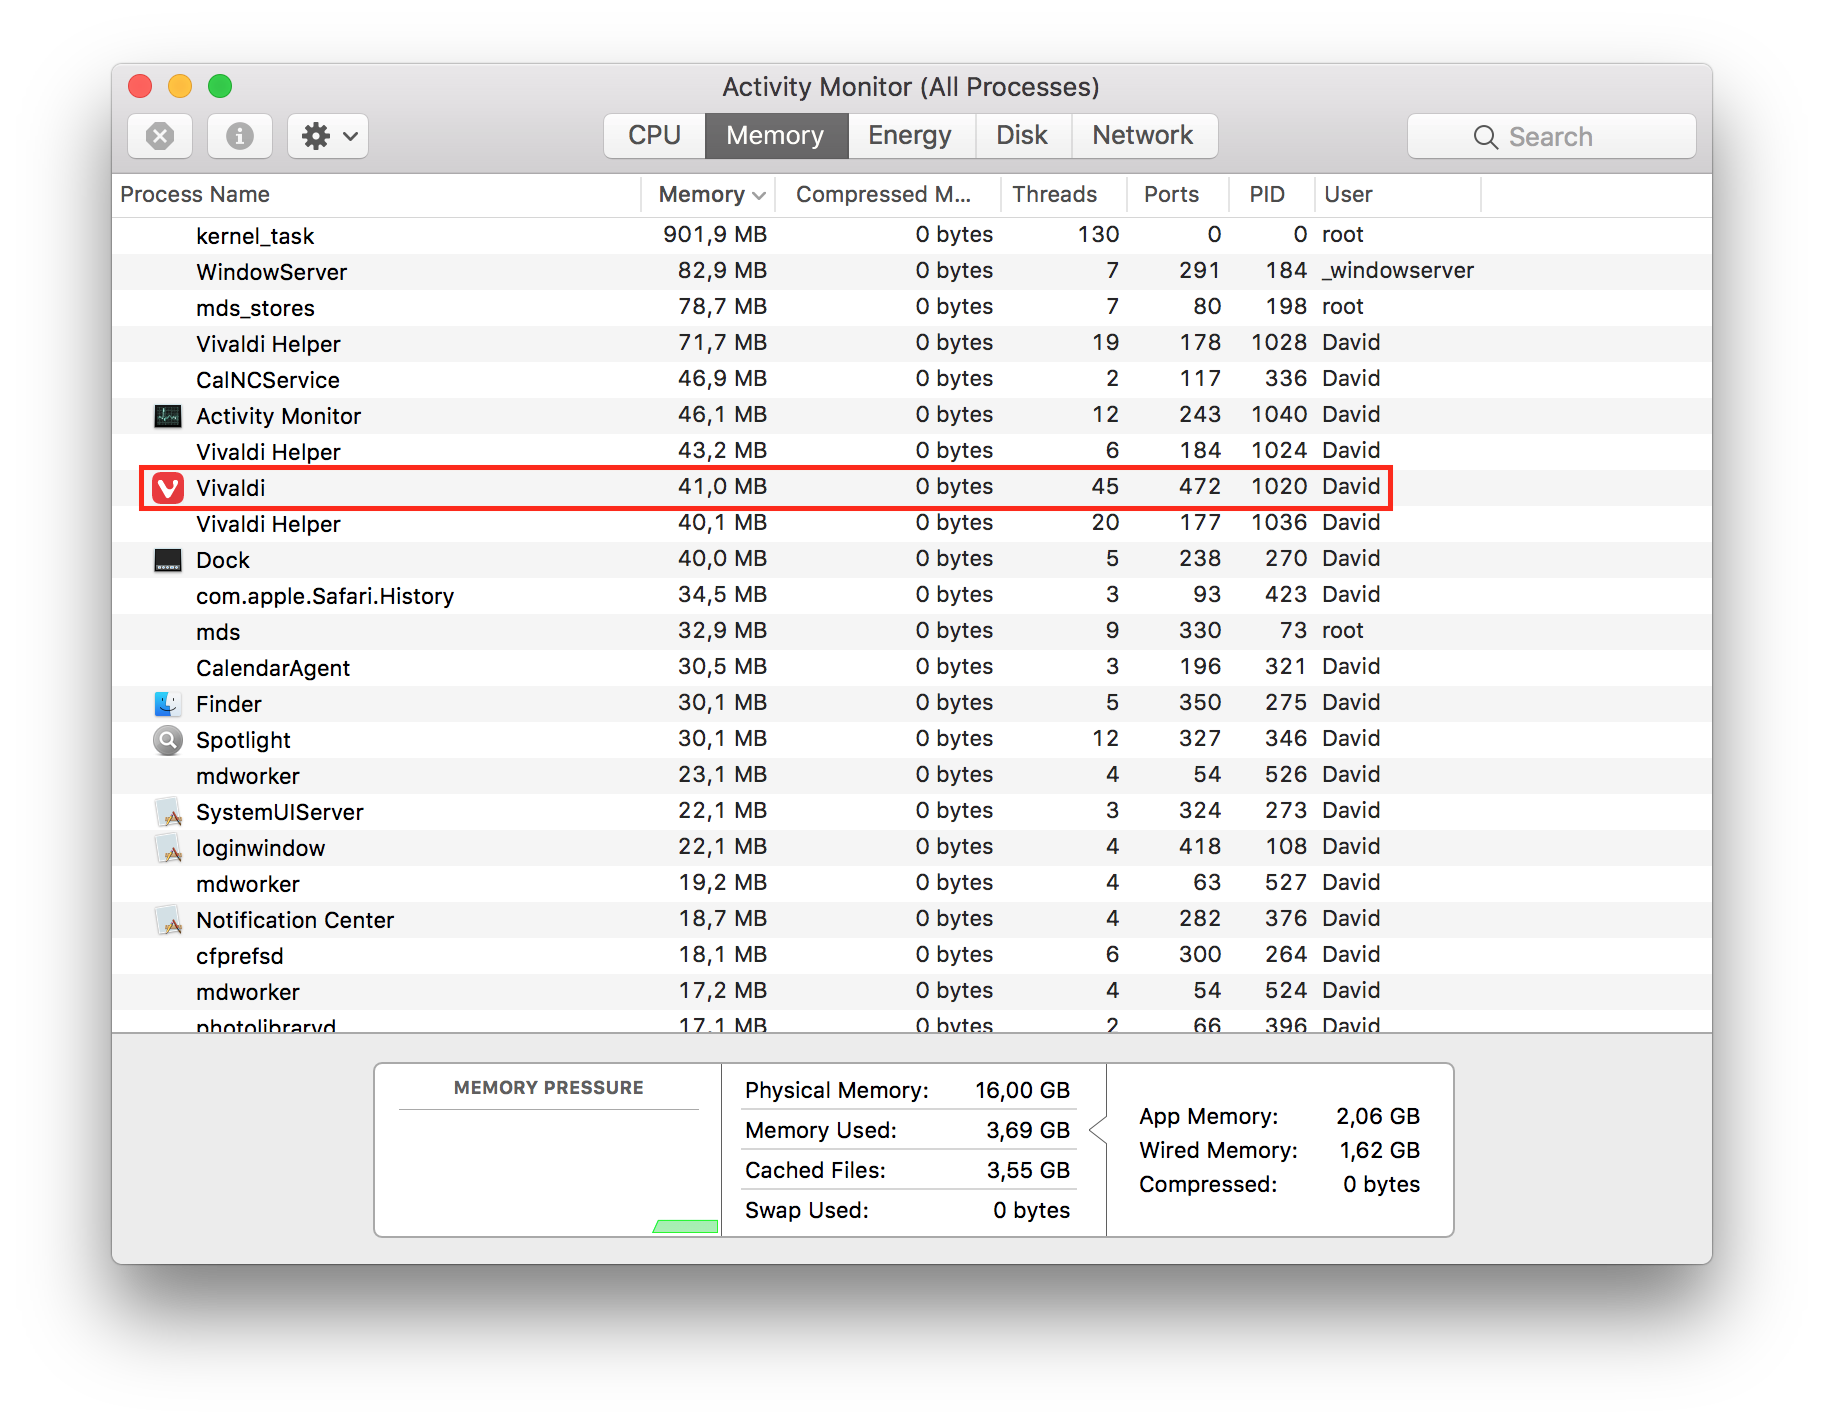
\includegraphics[width=0.75\linewidth]{./6_EvalEmpirica/Img/vivaldiRAM.png}
\end{center}
\caption{Consumo de RAM de Vivaldi para un computador MacOS.}
\label{vivaldiRAM}
\end{figure}

El consumo de RAM en Microsoft Edge, resaltado en rojo, es mucho menor. Dado que la transferencia de archivos de audio por la red ocurre de forma puntual y a intervalos muy cortos de tiempo, los indicadores de consumo de red son nulos en el momento de tomar la captura debido a que se encontraban entre envíos (Figura \ref{edgeRAM}).

\begin{figure}[!t]
\begin{center}
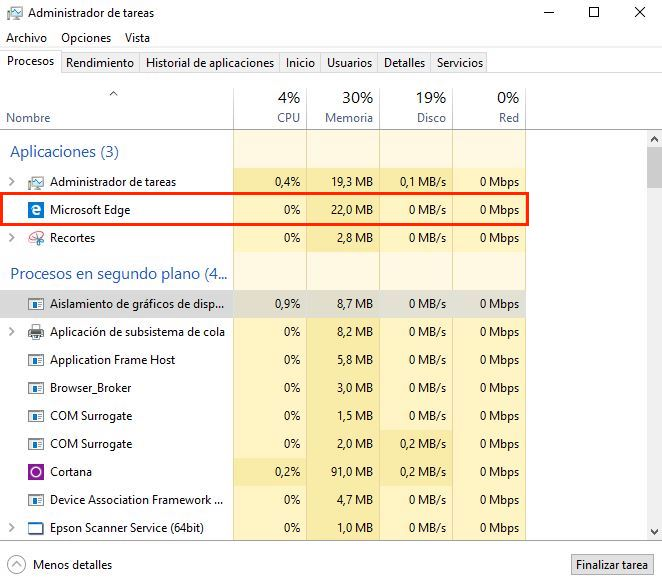
\includegraphics[width=0.75\linewidth]{./6_EvalEmpirica/Img/edgeRAM.jpg}
\end{center}
\caption{Consumo de RAM de Microsoft Edge para un computador con Windows.}
\label{edgeRAM}
\end{figure}

\subsection{Tráfico HTTP y TCP}

En una de las pruebas del sistema con el navegador de escritorio Firefox y cuando aún no se había implementado SSL se realizó una captura del tráfico con Wireshark. En la Figura \ref{traffic} se muestra el \emph{throughput} medio de la transmisión de audio desde el navegador al servidor, consistente en 45 tramas TCP de una longitud total de 64206 bits.

\begin{figure}[!t]
\begin{center}
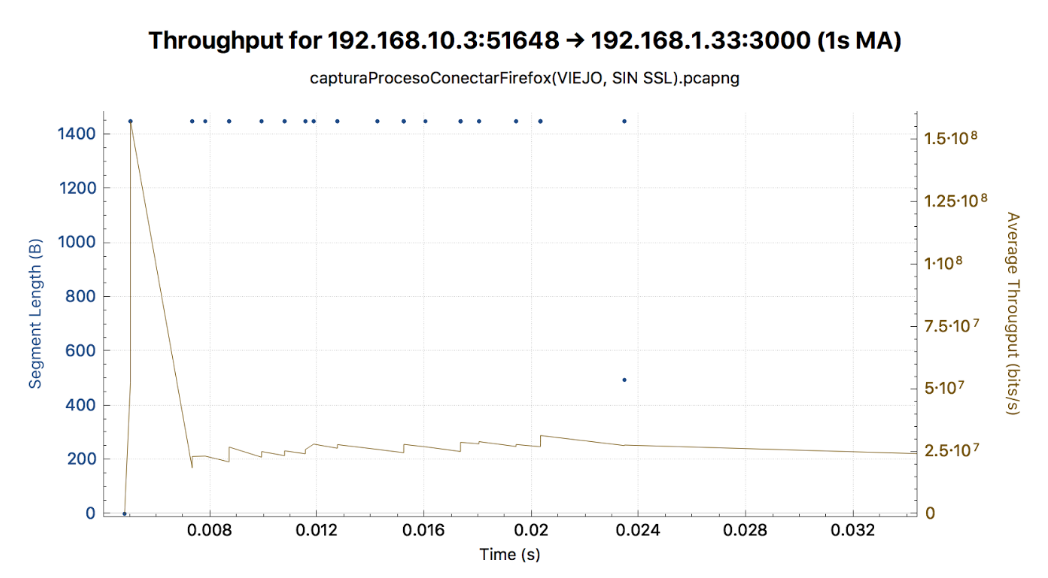
\includegraphics[width=0.75\linewidth]{./6_EvalEmpirica/Img/traffic.png}
\end{center}
\caption{Throughput de tráfico TCP y HTTP para comunicación de un archivo de audio.}
\label{traffic}
\end{figure}

Además, en las pruebas con sistemas de escritorio se realizó una prueba de velocidad del cliente conectado a través de nuestro sistema y se comparó con pruebas de velocidad cuando el usuario está conectado al mismo servicio contratado a la WiFi tradicional proporcionada por el equipo del operador. Las cifras para la conexión inalámbrica cuando se usa nuestro sistema en la comparativa descienden en 10 Mbps tanto en subida como en bajada, lo que es esperable dado que estamos añadiendo varias capas más de procesamiento a la transmisión (Figura \ref{speed}).

\begin{figure}[!t]
\begin{center}
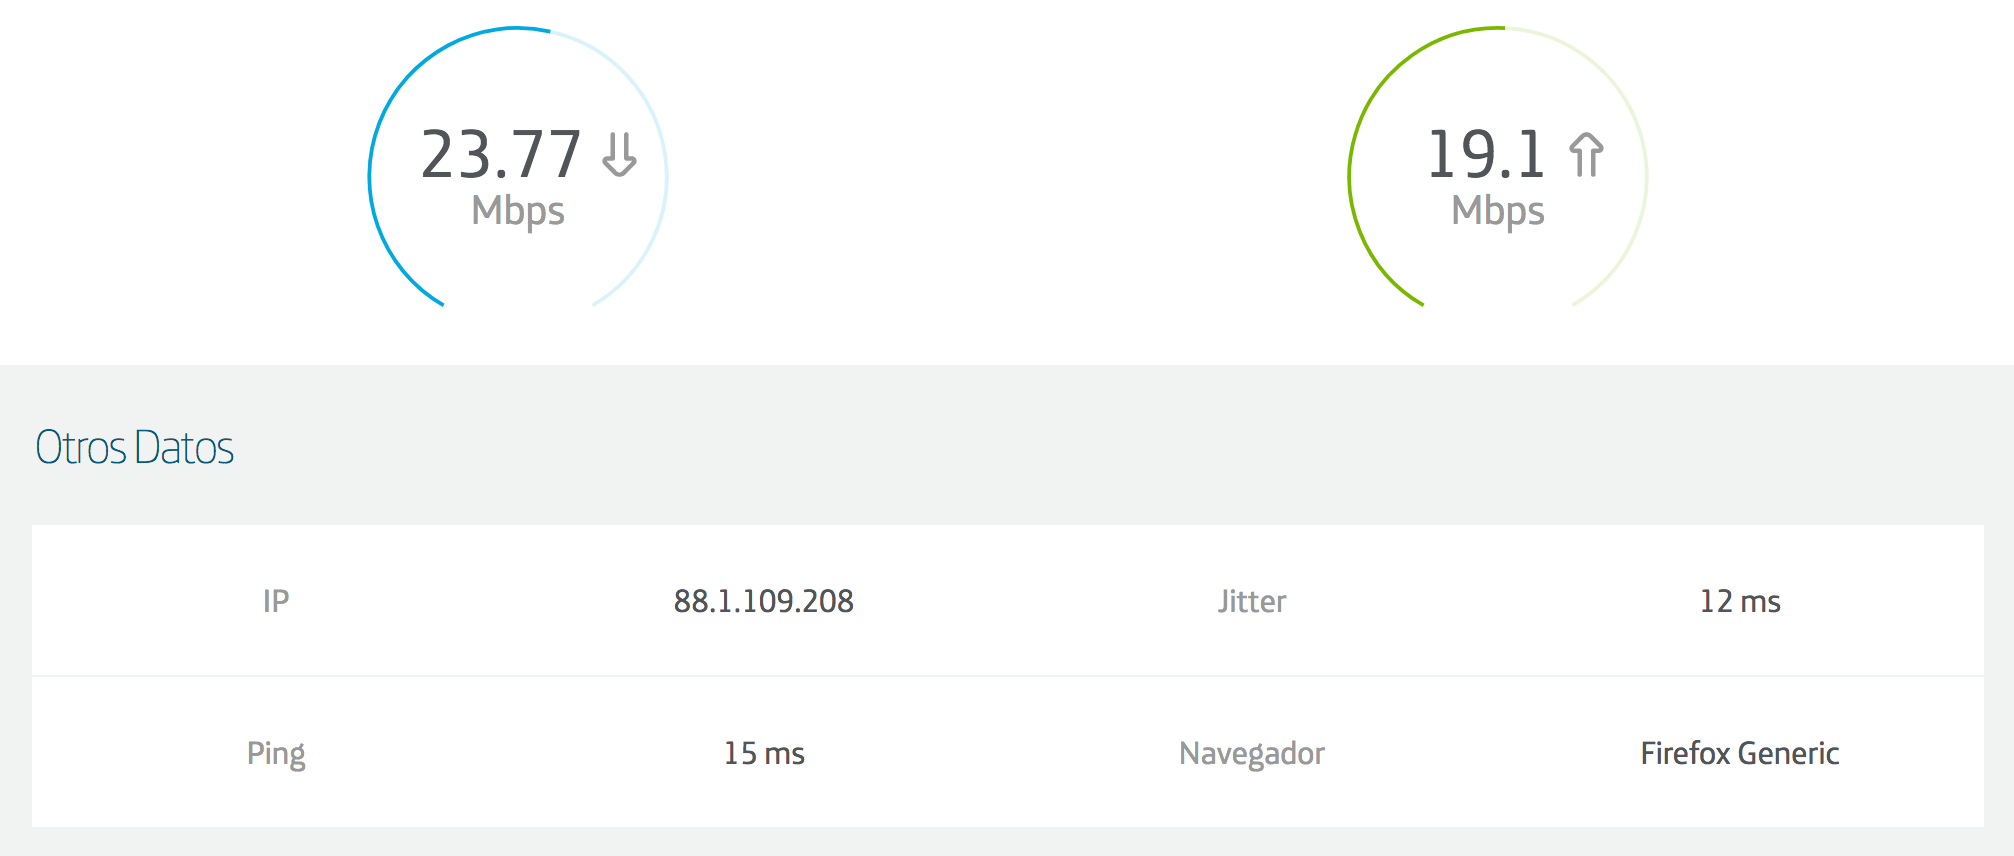
\includegraphics[width=0.75\linewidth]{./6_EvalEmpirica/Img/speed.png}
\end{center}
\caption{Prueba de velocidad de acceso a Internet a través de nuestro sistema.}
\label{speed}
\end{figure}

\subsection{Análisis de los archivos de audio generados}
Los archivos de audio generados y enviados al servidor son renombrados por la \emph{Aplicación Web} siguiendo la estructura de la Figura \ref{audioFiles}: el prefijo \emph{Lat} seguido de la latitud, el prefijo \emph{Lon} seguido de la longitud y el prefijo \emph{Time} seguido del \emph{timestamp} completo.

\begin{figure}[!t]
\begin{center}
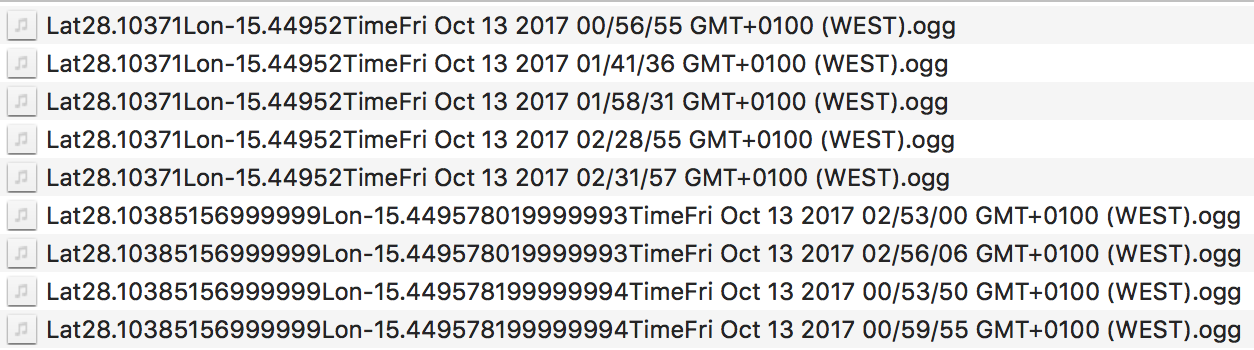
\includegraphics[width=0.75\linewidth]{./6_EvalEmpirica/Img/audioFiles.png}
\end{center}
\caption{Formato del archivo de audio etiquetado con geolocalización y temporización.}
\label{audioFiles}
\end{figure}

Cada archivo tiene una duración de 4 segundos, está codificado en \emph{Opus Audio} \cite{OpusCodec} y almacenado en un contenedor de formato \emph{Ogg}. La tasa de muestreo de la codificación es \emph{fullband} (48 kHz, como puede verse en la imagen). El fichero generado ronda los 63 KB de tamaño, lo que confirma lo apreciado en la captura del tráfico TCP correspondiente a un fichero enviado, de tamaño total ligeramente mayor y dividido en varias tramas (Figura \ref{audioInfo}).

\begin{figure}[!t]
\begin{center}
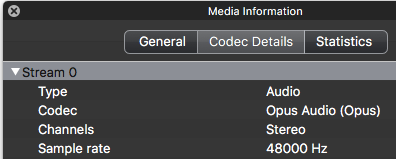
\includegraphics[width=0.75\linewidth]{./6_EvalEmpirica/Img/audioInfo.png}
\end{center}
\caption{Codificación del audio.}
\label{audioInfo}
\end{figure}
\cleardoublepage
\clearpage
\vspace*{\stretch{2}}%{\fill}
\begin{center}
\begin{minipage}{.75\textwidth}
\section{Conclusiones y posibles ampliaciones}

Presentados los resultados experimentales de la evaluación del sistema con distintos tipos de terminales móviles. En este capítulos presentamos las conclusiones principales así como posibles ampliaciones. % \pagebreak
\end{minipage}
\end{center}
\vspace{\stretch{3}} % \vfill % equivalent to \vspace{\fill}
\clearpage% https://tex.stackexchange.com/questions/70714/center-horizontally-and-vertically-a-block-of-text

\subsection{Conclusiones}
Se ha implementado un sistema de acceso a la red a cambio de audio recogido por el micrófono cuya interacción con los clientes se realiza de forma muy sencilla y sin hacer uso de aplicaciones o dispositivos externos al terminal, funcionando a través del navegador Web. El sistema al completo es transversal, ya que las diferentes módulo hardware y software utilizados se organizan en una arquitectura de niveles similar a la de la arquitectura de Internet. Además, para la Aplicación Web se han usado tecnologías en pleno desarrollo actual y con proyección de futuro como son Node.js y WebRTC.

Una vez probado en diversos dispositivos móviles de diferente tipo y gama (ordenadores, móviles y tablets) podemos determinar que el sistema desarrollado cumple con los objetivos planteados en la propuesta de TFG. Además, durante el desarrollo del mismo se ha adquirido gran familiaridad con las tecnologías implicadas, como las diferentes API y frameworks utilizados, y se ha comprobado cómo estas, particularmente las más recientes, evolucionan en el tiempo cambiando las condiciones actuales y futuras del sistema.

Un ejemplo de ello son las versiones de Node.js, que durante el desarrollo del TFG y en el momento de escribir esta conclusión pasaron de la 7 a la 9, introduciendo diversos cambios. Sin embargo, un ejemplo de hecho más relevante es la decisión de Apple de implementar soporte WebRTC en su motor de renderizado web, \emph{WebKit}, durante el desarrollo de este TFG, lo que ocasiona que desde la versión 11 de Safari, lanzado durante la escritura de este documento, algunas opciones de WebRTC puedan implementarse ahora en los dispositivos iOS. Lamentablemente, la API \emph{MediaStream Recording} que utilizamos en este TFG sigue sin tener soporte, pero es de esperar que tal y como sucedió con otros aspectos de WebRTC se empiece a trabajar en ello próximamente.

Un inconveniente de trabajar con tecnologías de este tipo es que, a diferencia de lo mencionado en el párrafo anterior, no todos los cambios introducidos son positivos. En cualquier momento podría lanzarse una nueva versión de la API y una revisión de los navegadores que obligue a los desarrolladores a modificar su proyecto o que complique el mantener una sintaxis de código final consistente.

\subsection{Posibles ampliaciones futuras}

Existen varios aspectos a tener en cuenta a la hora de llevar a cabo este proyecto. A continuación se detallan algunos de ellos junto a posibles ampliaciones que pueden llevarse a cabo en el futuro.

%\subsubsection{Replicabilidad}

En este Trabajo Fin de Grado se detalla paso a paso cómo conseguir el producto final, descargando y configurando todo el software y realizando el código desde cero. Sin embargo, el hecho de que el sistema esté implementado sobre una Raspberry Pi 3 permite replicar el sistema con gran facilidad. Al estar el sistema operativo en su totalidad almacenado en una tarjeta MicroSD, puede obtenerse un archivo imagen de esta y luego clonarse en todas las tarjetas de este tipo que se desee, obteniendo múltiples copias del sistema en las que solo haría falta modificar unos pocos archivos y configuraciones (como el archivo \emph{config} de CoovaChilli o la contraseña del usuario \emph{root} de Raspbian) para adecuarlo a las necesidades específicas de la implementación.

%\subsubsection{Privacidad}

La privacidad se ha convertido en uno de los elementos más cruciales, analizados y debatidos en el campo de las tecnologías de la información y la comunicación. El sistema desarrollado en este TFG está diseñado para capturar una muestra de audio de los usuarios del servicio cada cierto tiempo, almacenando a priori un tipo de información potencialmente sensible en un servidor ajeno. En las implementaciones de este servicio el usuario debería ser plenamente consciente de lo que está ocurriendo con la información que se obtendría de él, por lo que es ético que la información ofrecida en el portal cautivo y las condiciones de uso sean lo más transparentes posibles para el usuario final.

Otra opción, que queda fuera del ámbito de este trabajo, es el cifrado de los datos transferidos o el uso de otras herramientas de anonimización que puedan emplearse a la hora de implementar el servicio, o que directamente el audio no sea transferido, sino que según las necesidades del sistema (como por ejemplo si solo se desea obtener el nivel de intensidad sonora) este sea procesado directamente en la \emph{Aplicación Web} y se transmita tan solo un valor o resultado numérico que no proporcione información sensible sobre el usuario.

%\subsubsection{Procesado del audio obtenido}

Aunque en un principio se deseaba entrar en este aspecto, las restricciones de tiempo hicieron imposible dedicar recursos a los posibles procesados de los archivos de audio generados por el sistema. A continuación se mencionan algunos de estos posibles usos.

\begin{itemize}
\item \emph{Mapeo de nivel de audio}: uno de los usos más inmediatos que son posibles en este sistema es el de realizar mapas de ruido en el área de cobertura del punto de acceso utilizando los ficheros generados y la información de ubicación que les acompaña. La información de estos mapas de nivel puede volverse más fiable si existen varios puntos de acceso que tomen medidas de dispositivos cliente cercanos. En estos casos, sería conveniente también obtener la información del dispositivo que ha grabado el audio para poder aplicar las correcciones y ponderaciones pertinentes a la muestra.
\item \emph{Localización acústica}: si contamos con varios puntos de acceso y grupos de usuarios cercanos entre sí en los que haya al menos un usuario conectado a cada punto (algo que podría lograrse con técnicas de balance de carga) podrían utilizarse técnicas de procesado de señal para intentar obtener la ubicación de estos grupos de forma acústica, atendiendo a la diferencia de fase e intensidad de las señales obtenidas. En estos casos podemos prescindir del servicio de geolocalización que nos proporciona el navegador web, utilizado en nuestro sistema, o continuar usándolo para realizar comparativas.
\end{itemize}

%\subsubsection{Desacoplar procesos}

El \emph{hardware} de acceso a la red y el servidor web pueden implementarse en sistemas separados, tales como un \emph{gateway} dedicado al acceso a la red y un servidor del portal cautivo y la gestión de AAA. Mediante el uso del \emph{software} mencionado anteriormente (\emph{iptables}, \emph{dnsmasq}…) puede obtenerse un mayor control sobre las conexiones y el ancho de banda utilizado, separándolo por ejemplo en grupos de usuarios, varias redes, filtrando por MAC, implementando redes privadas con VPN… todo ello sin tener que recurrir a CoovaChilli.

%\subsubsection{Unificar \emph{software}}
Por el contrario, se puede seguir con un dispositivo \emph{hardware} único conectado a la red y centralizar toda la gestión en Node.js, haciendo que este sirva el portal cautivo y también dé de alta a los usuario en la red accediendo directamente a la base de datos e incluso ejecutando los órdenes o \emph{scripts} de \emph{iptables} directamente. Esto incrementaría la complejidad de la aplicación Node.js pero se obtendría a cambio una gestión centralizada del sistema al completo, ahorrando en elementos potencialmente superfluos como las bases de datos de usuarios intermedias que existen en la implementación actual.



\cleardoublepage
%\bookmarksetup{startatroot}
\begin{appendices}
%\addtocontents{toc}{\protect\setcounter{tocdepth}{0}}
%\appendix
\clearpage
\vspace*{\stretch{2}}%{\fill}
\begin{center}
\begin{minipage}{.75\textwidth}
\section{Instalación del \emph{hardware} necesario}\label{ApendiceA}


Una vez revisado el análisis previo y funcional del sistema de sensado móvil colaborativo mediante un visión \emph{top-down}, en este capítulo presentamos  el análisis orgánico de la implantación mediante una visión \emph{bottom-up}. Esto es, primero se configura el nivel inferior, la capa del \emph{hardware} y el Control de Red, tras lo cual se va ascendiendo en el modelo hasta llegar a la implantación del portal cautivo, en la capa de Usuarios y el nivel más alto del sistema total.
\end{minipage}
\end{center}
\vspace{\stretch{3}} % \vfill % equivalent to \vspace{\fill}
\clearpage% https://tex.stackexchange.com/questions/70714/center-horizontally-and-vertically-a-block-of-text

\sloppy

En este Apéndice se asume que se dispone de conexión a Internet operativa a la que la Raspberry Pi 3 pueda conectarse (cableada o inalámbrica) y un ordenador de trabajo, no entrando en detalles sobre su configuración por entender que no es parte del TFG.

Para poner en marcha la Raspberry Pi 3 de forma sencilla es necesario disponer de la propia placa, una fuente de alimentación USB Micro (un adaptador de corriente como el de la mayoría de teléfonos móviles actuales), teclado y ratón, una tarjeta microSD de al menos 8 GB clase 4 y un monitor con entrada HDMI, para lo que puede servir una pantalla de televisión. También hace falta disponer de conexión a Internet, ya sea mediante red cableada o una red inalámbrica a la que la Raspberry Pi 3 pueda conectarse.

La tarjeta microSD debe de tener ya almacenado el sistema operativo Raspbian desde el principio o por el contrario hacer uso de la solución recomendada desde la propia página Web oficial, la herramienta \emph{New Out Of Box Software} (\emph{\acrshort{NOOBS}}, que en inglés significa \emph{novatos}). Esta herramienta es un gestor de instalaciones de sistemas operativos para la Raspberry Pi, disponible desde su página Web oficial. Puede comprarse la tarjeta SD con dicha herramienta preinstalada o puede instalarse manualmente haciendo uso de un ordenador, descargando el archivo comprimido de NOOBS y descomprimiéndolo en una tarjeta SD vacía y formateada en FAT32, de forma que los archivos estén en el directorio raíz de la tarjeta. Tras este proceso la tarjeta queda preparada para funcionar insertándose en la Raspberry Pi 3, enchufando la misma al teclado, ratón y monitor y por último a la corriente eléctrica.

Al ser enchufada a la corriente la Raspberry Pi se inicia de forma automática y carga la herramienta NOOBS, tras lo que aparece la pantalla de selección de sistemas operativos en el que debemos seleccionar Raspbian (Figura \ref{NOOBS}) y pulsar el botón \emph{Instalar} en la esquina superior izquierda del menú, tras lo cual comienza el proceso de instalación de Raspbian utilizando la totalidad de la tarjeta microSD para su sistema de archivos (si utilizamos la versión ligera de NOOBS primero se efectúa la descarga del mismo, ya que no vendría incluido en la herramienta). Al terminar, la herramienta avisa y se procede al reinicio del dispositivo.

\begin{figure}[!t]
\begin{center}
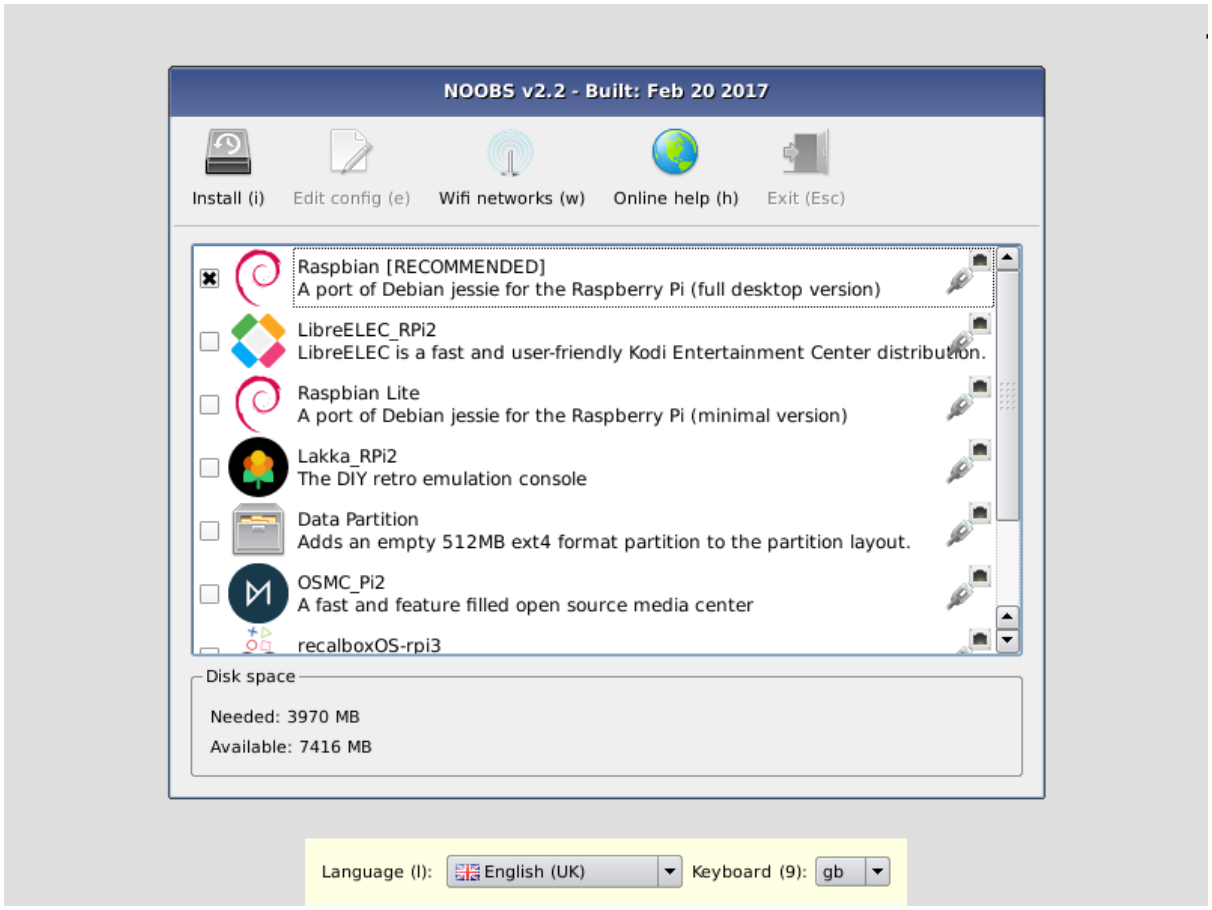
\includegraphics[width=0.75\linewidth]{./X_Anexos/Img/NOOBS.png}
\end{center}
\caption{Selección de Raspbian para ser instalado en la Raspberry Pi 3.}
%\source{https://en.wikipedia.org/wiki/RADIUS}
\label{NOOBS}
\end{figure}

Tras la instalación de Raspbian la herramienta NOOBS sigue estando disponible como partición de recuperación para la Raspberry Pi 3, accesible pulsando la tecla \emph{shift} en el momento de encendido al aparecer por primera vez el logotipo de Raspberry Pi.

Aunque su implantación queda fuera del ámbito de este TFG, la Raspberry Pi cuenta con una serie de interfaces activables desde el entorno gráfico o la orden de terminal \emph{raspi-config} que permiten su gestión remota, ya sea mediante \emph{Secure Shell} (\acrshort{SSH}) o servidores \emph{Virtual Network Computing} (\acrshort{VNC}) \cite{RasPiVNC}, tras lo que la Raspberry Pi podría ser manejada en modo headless, sin estar conectada a teclado, ratón o salida de vídeo, tan solo a la corriente y a una red local por medio de alguna de sus interfaces de red.

No entramos en la configuración del hardware de la WiFi de la Raspberry Pi 3 porque ya viene instalada por defecto en Raspbian.

En este apartado no entramos en el detalle de la configuración de \emph{hostapd} porque en el capítulo 5 presentamos toda la instalación del software necesario por orden de dependencias entre ellos, lo cual nos obligaría a explicar previamente aplicaciones que pertenecen a otros módulos.
\clearpage
\vspace*{\stretch{2}}%{\fill}
\begin{center}
\begin{minipage}{.75\textwidth}
\section{Descarga automática del código de la Nube}\label{ApendiceB}

Hoy en día la tendencia es a alojar los proyectos de libre distribución y código abierto en la Nube. Nosotros hemos alojado nuestro proyecto en la nube \emph{GitHub}. En este apéndice proporcionamos la dirección Web de acceso a él y la instalación automática de todo el entorno.
\end{minipage}
\end{center}
\vspace{\stretch{3}} % \vfill % equivalent to \vspace{\fill}
\clearpage% https://tex.stackexchange.com/questions/70714/center-horizontally-and-vertically-a-block-of-text

Para implementar el servicio, en lugar de replicar el código manualmente, puede clonarse el repositorio online habilitado explícitamente para ello mediante la herramienta de control de versiones \emph{git}, situándose en el directorio donde se quiera almacenar los archivos y ejecutando la siguiente orden en el terminal: 

\mint{bash}{git clone https://github.com/DavSanchez/CaptivePortal.git}

Tras esto, el servicio Web completo puede ponerse en marcha desde este mismo directorio mediante el orden node.

\mint{bash}{node nodeserver.js}
\clearpage
\vspace*{\stretch{2}}%{\fill}
\begin{center}
\begin{minipage}{.75\textwidth}

\section{Reanudación automática del Servidor en caso de fallo}\label{ApendiceC}

Proporcionando la orden de arranque del Apéndice \ref{ApendiceB} (\mintinline{bash}{node nodeserver.js}) es suficiente para que el sistema de sensado móvil colaborativo arranque y proporcione los servicios desarrollados. sin embargo, se puede dar el caso de fallos del servidor en cuyo caso debemos tolerarlos. En este apéndice se explica como hacerlo.
\end{minipage}
\end{center}
\vspace{\stretch{3}} % \vfill % equivalent to \vspace{\fill}
\clearpage% https://tex.stackexchange.com/questions/70714/center-horizontally-and-vertically-a-block-of-text

La orden ejecutada justo al final del apartado anterior basta para poner en marcha el servicio, pero no protege ante la situación de que un fallo detenga su ejecución y requiere que un administrador lo ejecute siempre que el hardware se pone en marcha. Existen diversas utilidades para solucionar esta situación no deseada; la utilizada en este TFG es PM2.

PM2 es un gestor de procesos para Node.js que nos permite configurar el comportamiento del servicio Web implementado frente a cambios en los archivos locales (como una actualización) u otras situaciones. Puede instalarse a través del gestor de paquetes \emph{npm}:

\mint{bash}{npm install pm2 -g}

Tras instalar esta herramienta ejecutaríamos una serie de órdenes con ella que nos permiten reanudar la aplicación Node.js de forma automática nada más encender nuestra Raspberry Pi 3, reiniciando el servicio si ocurre algún error o incluso si actualizamos el código de forma local o remota (editándolo en otra parte, subiéndolo a GitHub y recuperándolo con la orden \mintinline{bash}{git pull}): 

\mint{bash}{pm2 startup}

Esta orden detecta el sistema en el que nos encontramos y nos recomienda el orden a ejecutar para generar un \emph{startup script}, que es ejecutado nada más encender el dispositivo. Una salida de ejemplo de este orden es la siguiente:

\begin{listing}[H]
\begin{minted}
[
frame=lines,
framesep=2mm,
baselinestretch=1.2,
bgcolor=lightgray,
fontsize=\footnotesize,
breaklines=true,
breaksymbolleft={}
]
{bash}
[PM2] You have to run this command as root. Execute the following command:
      sudo su -c "env PATH=$PATH:/home/unitech/.nvm/versions/node/v4.3/bin pm2 startup <distribution> -u <user> --hp <home-path>
\end{minted}
\caption{PM2 sugiere un comando a introducir para poder ejecutarse al iniciar el sistema.}
\label{startupScript}
\end{listing}

Tras este proceso, solo queda configurar los parámetros a usar por PM2, ejecutar las aplicaciones Node.js deseadas y guardar el entorno con la siguiente orden:

\mint{bash}{pm2 save}

Este paso asegura que la aplicación Node.js vuelve a ejecutarse tras un reinicio del sistema, ya sea un reinicio programado o el ocurrido tras un corte accidental.

Para conseguir lo anterior es necesario configurar el entorno de programación. Para ello se puede utilizar un archivo de configuración como el empleado en este TFG, ubicado en la raíz del repositorio de GitHub con el nombre \verb+captiveportalserver.config.js+. El contenido de este archivo es el siguiente:

\begin{listing}[H]
\begin{minted}
[
frame=lines,
framesep=2mm,
baselinestretch=1.2,
bgcolor=lightgray,
fontsize=\footnotesize,
breaklines=true,
breaksymbolleft={}
]
{javascript}
module.exports = {
 apps : [
   {
     name      : "nodeserver",
     script    : "./nodeserver.js",
     watch     : true,
 ignore_watch: ["./.git", "./node_modules", "./.gitignore", "./uploads", "./users/users.json", "./users/usersOneTime.json"]
   }
 ]
}
\end{minted}
\caption{Fichero de configuración del entorno node con PM2}
\label{PM2Env}
\end{listing}

Se observa que se trata esencialmente de un objeto JavaScript con los siguientes campos:

\begin{itemize}
\item \emph{name}: el nombre asignado al proceso.
\item \emph{script}: la ubicación del archivo Node.js que ejecutaríamos normalmente con la orden \emph{node}.
\item \emph{watch}: un flag que vigila cambios en nuestros archivos, reiniciando la aplicación Node.js si se detectara uno.
\item \emph{ignore\_watch}: \emph{Array} de archivos y directorios que no se vigilan con el \emph{flag} anterior.
\end{itemize}

Si nuestro entorno requiriese de más aplicaciones Node.js ejecutadas simultáneamente podrían añadirse como nuevas instancias del objeto \emph{apps}.

Una vez terminada la configuración de nuestro entorno, lo ejecutamos mediante PM2 (no mediante node) y guardamos el entorno tal y como se nos queda para que se ejecute de la siguiente forma cada vez que se inicie nuestro sistema.

\mint{bash}{pm2 start captiveportalserver.config.js}
\mint{bash}{pm2 save}

Por último, con la orden \mintinline{bash}{pm2 monit} puede accederse a una vista de monitorización que nos permite ver una lista de las aplicaciones activas y su consumo en memoria, la salida en consola de cada una de ellas, el número de veces que se han reiniciado (Figura \ref{pm2monit}).

\begin{figure}[!t]
\begin{center}
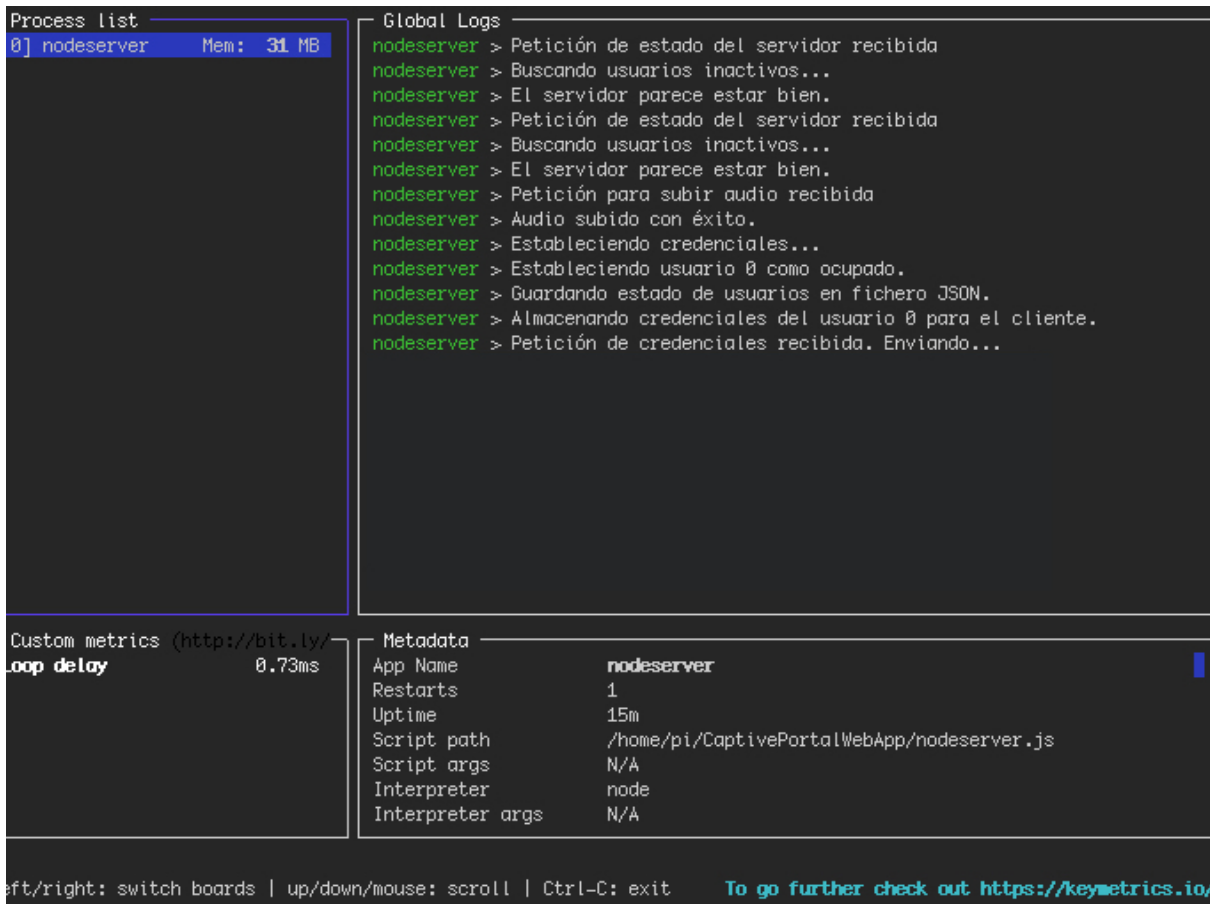
\includegraphics[width=0.75\linewidth]{./X_Anexos/Img/pm2monit.png}
\end{center}
\caption{Vista de monitorización de aplicaciones activas con pm2 monit.}
%\source{https://en.wikipedia.org/wiki/RADIUS}
\label{pm2monit}
\end{figure}
\clearpage
\vspace*{\stretch{2}}%{\fill}
\begin{center}
\begin{minipage}{.75\textwidth}
\section{Ciclo de Vida del TFG}\label{ApendiceD}

En este apéndice se presenta una visión rápida del ciclo de vida del TFG. El objetivo es mostrar cómo ha ido evolucionando la implantación del sistema de sensado.
\end{minipage}
\end{center}
\vspace{\stretch{3}} % \vfill % equivalent to \vspace{\fill}
\clearpage% https://tex.stackexchange.com/questions/70714/center-horizontally-and-vertically-a-block-of-text

El desarrollo de este TFG no consistió en considerar un único curso de acción y desarrollar la solución. Durante las etapas iniciales se tuvieron en cuenta e investigaron varias alternativas con el objetivo de llegar al mismo resultado final, elementos que se vieron reflejados en los mecanismos de seguimiento presentados. A continuación detallamos algunos de estas primeras aproximaciones y se explica el motivo de haberlas declinado en favor del camino finalmente escogido.

La primera solución propuesta para el TFG, apareciendo así en la primera versión de la propuesta o anteproyecto, consistía en programar una aplicación nativa para terminales Android que gestionara la captura del audio y la ubicación, habilitando el acceso a Internet una vez transferidos los archivos al servidor. Esta solución podría extenderse más adelante a sistemas iOS. Se pensó también implementar una aplicación universal mediante un \emph{wrapper} como \emph{Apache Cordova}, la tecnología anteriormente conocida como \emph{PhoneGap}, con lo que con una sola programación se podrían obtener aplicaciones para diversos sistemas móviles.

Sin embargo, la propuesta de aplicación nativa resultaba altamente situacional, implicando que un hipotético usuario del servicio tuviera una aplicación instalada en su dispositivo de antemano si quería poder acceder a la red. Además, el desarrollo de aplicaciones nativas orientadas a terminales móviles excluía a los ordenadores portátiles, que sin ser \emph{smartphones} ni \emph{tablets} debían poder utilizar el servicio sin problema. Este enfoque requeriría entonces programar aplicaciones de escritorio separadas o implementar alguna otra solución específica para ellos, lo que alargaría el proceso de programación.

Finalmente, con el objetivo de facilitar lo más posible la implementación y el acceso al servicio, junto a la oportunidad de utilizar tecnologías de aparición reciente como las API de \emph{WebRTC}, se optó por desarrollar una aplicación web, accesible desde cualquier dispositivo que cuente con un navegador compatible.

Para implementar el servidor se pensó desde el primer momento en utilizar la Raspberry Pi. Pese a que se disponía de unas cuantas en su modelo 2 y se intentó implementar en ellas, estas carecen de \emph{chipset} WiFi propio, por lo que se debía adquirir por separado, conectarse a esta por USB y compilar el controlador del \emph{hardware} utilizado. Además, no todos los dispositivos WiFi externos disponibles soportan trabajar en modo punto de acceso indispensable para nuestro proyecto, por lo que había que tener especial cuidado al adquirir uno de ellos. Con el objetivo de ahorrarnos toda esta problemática se decidió trabajar directamente con la Raspberry Pi 3, que ya incluye \emph{chipset} WiFi 802.11n propio capaz de trabajar en el modo deseado, teniendo además el mismo precio que su modelo predecesor. Al igual que se tuvieron en cuenta varias alternativas para la implementación del lado del cliente, se experimentó con diversas posibilidades para el lado del servidor en la Raspberry Pi hasta optar por la escogida finalmente.

Durante el proceso de documentación, previa a la implementación del TFG se pensó en implantar el control de acceso a la red manualmente. Para ello se contemplaron diversas opciones para servidores DHCP (como \emph{dnsmasq} o \emph{isc-dhcp-server}) que proporcionarían direccionamiento IP a los dispositivos conectados. Junto a estos actuaría la utilidad de Linux \emph{iptables}, que permite establecer reglas para el procesamiento de paquetes IP, pudiendo aplicarse permanentemente a través del paquete \emph{iptables-persistent} o mediante \emph{scripts} que se ejecutarían y aplicarían las reglas al iniciar el sistema operativo. Sin embargo, este último paquete presentó problemas al ser instalado en la Raspberry Pi, por lo que esta opción fue descartada al poco tiempo de descubrir la solución que proporcionaba CoovaChilli.

En cuanto a los servidores Web para alojar el portal cautivo, inicialmente se pensó en utilizar un enfoque tradicional con servidores como \emph{Apache}, \emph{Nginx} o soluciones ligeras como \emph{lighttpd} junto a PHP o \emph{web scripts} CGI. Finalmente fueron parcialmente descartados como implementación principal en favor de tecnologías web de gran popularidad actual como Node.js, usando el servidor web Nginx solamente para alojar la interfaz web daloRADIUS.

Aunque Raspbian es la oficial, la Raspberry Pi permite instalar otras distribuciones y sistemas operativos. Uno de ellos es \emph{OpenWRT}, una solución de código abierto para sistemas empotrados orientados a encaminamiento de tráfico de red. Puede instalarse en pasarelas residenciales, ordenadores portátiles e incluso teléfonos móviles, por lo que su instalación es viable en la Raspberry Pi. OpenWRT tiene disponible una gran cantidad de protocolos como DNS y DHCP, \acrshort{NAT}, mapeo de puertos, aplicaciones de seguridad... también es posible el uso de portales cautivos instalando \emph{CoovaChilli}.

Finalmente se decidió no optar por esta solución debido a que la distribución basada en \emph{Debian} predeterminada para la Raspberry Pi ofrece un soporte más amplio en cuanto a documentación y mayores posibilidades para implementar otras tareas relacionadas con el proyecto: gestión, análisis y procesado de los ficheros de audio, simulaciones de ubicación acústica...

Junto a CoovaChilli se evaluó otra solución de control de acceso a la red disponible para Linux: \emph{PacketFence}. Este programa de código abierto es también muy completo, ofreciendo facilidades de monitorización, análisis de ficheros transmitidos, gestión centralizada tanto cableada como inalámbrica (802.1X) y utilidades de portal cautivo. Lamentablemente, cuando se estudió su uso \emph{PacketFence} no garantizaba compatibilidad total para la Raspberry Pi, por lo que también fue descartado.

\clearpage
\vspace*{\stretch{2}}%{\fill}
\begin{center}
\begin{minipage}{.75\textwidth}
\section{Problemas Acontecidos durante el Desarrollo de la Solución}\label{ApendiceE}

En este apéndice se presentan algunas dificultades ocurridas durante el desarrollo del TFG que limitaron el diseño del sistema final y alargaron en el tiempo desarrollos que a priori no tenían dificultad.
\end{minipage}
\end{center}
\vspace{\stretch{3}} % \vfill % equivalent to \vspace{\fill}
\clearpage% https://tex.stackexchange.com/questions/70714/center-horizontally-and-vertically-a-block-of-text

Uno de los problemas a los que nos enfrentamos a la hora de implementar este TFG es el de los navegadores compatibles con WebRTC. La API \emph{MediaStream Recording} utilizada aún no está soportada por todos los navegadores, siendo Safari, navegador de los dispositivos Apple, el ejemplo más relevante de esta falta de soporte. Este problema es mayor de lo que parece debido a que Apple obliga a que todos los navegadores disponibles en la App Store de iOS hagan uso del motor de renderizado web WebKit que también usa Safari, por lo que en un dispositivo iOS no podemos simplemente cambiar de navegador para que nuestro sistema funcione.

Aunque no presenta problema a la hora de ser probado en local, las API de geolocalización y de grabación multimedia requieren de un contexto seguro. Esto implica que el sistema no funciona sin hacer uso de HTTPS, por lo que hubo que implementar este sistema en nuestra aplicación web haciendo uso de la herramienta OpenSSL, la API correspondiente para \acrshort{HTTPS} en Node.js y habilitar esta opción en CoovaChilli.

Dado que OpenSSL genera certificados auto-firmados, y por tanto no reconocidos por una autoridad de certificación, los navegadores no los aceptan de primeras para proteger al usuario, por lo que a efectos de hacer las pruebas hubo que añadir las excepciones de la aplicación web y la interfaz JSON de \emph{CoovaChilli} manualmente.

\clearpage
\vspace*{\stretch{2}}%{\fill}
\begin{center}
\begin{minipage}{.75\textwidth}
\section{Tabla de Desarrollo Temporal}\label{ApendiceF}

Se presenta una tabla de desarrollo temporal.
\end{minipage}
\end{center}
\vspace{\stretch{3}} % \vfill % equivalent to \vspace{\fill}
\clearpage% https://tex.stackexchange.com/questions/70714/center-horizontally-and-vertically-a-block-of-text

La cronología de desarrollo aproximado del proyecto se muestra en la Tabla \ref{tablaTFG}.

\begin{table}[!ht]
\begin{center}
\begin{tabular}{ | l | c | }
\hline
\textbf{Tarea acometida} & \textbf{Tiempo invertido} \\
\hline
Documentación inicial & 10 horas \\ \hline
Especificación & 10 horas \\ \hline
Opciones consideradas & 10 horas \\ \hline
Análisis software de servidor & 20 horas \\ \hline
Diseño final & 20 horas \\ \hline
Implementación final (WebApp + Server) & 160 horas \\ \hline
Pruebas en Raspberry Pi 2 + Interfaz WiFi & 5 horas \\ \hline
Configuración de Seguridad HTTPS & 5 horas \\ \hline
Pruebas en Raspberry Pi 3 & 10 horas \\ \hline
Correcciones y cambios & 20 horas \\ \hline
Pruebas finales & 20 horas \\ \hline
Elaboración de documentos finales & 10 horas \\ \hline
\end{tabular}
\end{center}
\caption{Cronología aproximada de realización del TFG}
\label{tablaTFG}
\end{table}%

\end{appendices}
\cleardoublepage

% Referencias, para crearlas compilamos primero ESTE documento en LaTeX,
% luego, lo compilamos en BibTeX o BibTaTeX (pillará el documento .bib referenciado en bibliography)
% finalmente, compilamos en LaTeX DOS VECES.

\nocite{*}
\printbibliography[title={Referencias},nottype=online, heading=bibintoc]%
\printbibliography[title={Referencias Web}, type=online, heading=bibintoc]%
\cleardoublepage

%\clearpage
\vspace*{\stretch{2}}
\begin{center}
\begin{minipage}{.75\textwidth}
\section*{Presupuesto}
\addcontentsline{toc}{section}{Presupuesto}

En este apartado se hace balance de los costes totales de llevar a cabo este Trabajo Fin de Grado. En el presupuesto se distinguen 3 partidas fundamentales de gasto: recursos materiales, costes de ingeniería y costes en bienes fungibles.
\end{minipage}
\end{center}
\vspace{\stretch{3}}
\clearpage

\subsection*{Coste de recursos materiales}
\addcontentsline{toc}{subsection}{Coste de recursos materiales}

Aquí se detallan los gastos dedicados a los recursos materiales utilizados para desarrollar este TFG. El total de gasto en recursos materiales es de $461.68$\euro. A continuación se detalla cada partida de gasto.

\subsubsection*{Recursos \emph{hardware}}
\addcontentsline{toc}{subsubsection}{Recursos \emph{hardware}}

Considerando una amortización lineal a 3 años de los equipos utilizados durante el tiempo de desarrollo del TFG, en la siguiente tabla se detalla el coste de cada elemento.

 \begin{table}[!ht]
     \begin{center}
     \begin{tabular}{| l  r  r |}
     \hline
     \textbf{Elemento} & \textbf{Coste total (\euro)} & \textbf{Coste imputable (\euro)} \\
     \hline
     Ordenador MacBook Pro 15'' & $1500$ & $333.3$ \\ %\hline
     Tablet Samsung Galaxy GT-P5210 & $150$ & $33.3$ \\ %\hline
     Móvil Sony Xperia L & $350$ & $77.78$ \\ %\hline
     Raspberry Pi 3 y accesorios & $89$ & $17.3$ \\ \hline
\multicolumn{1}{| r }{\textbf{Total}} & & \textbf{$461.68$\euro} \\ \hline
     \end{tabular}
     \end{center}
     %\caption{Coste total del \emph{hardware}}
     \label{costeHard}
     \end{table}%
     
\subsubsection*{Recursos \emph{software}}
\addcontentsline{toc}{subsubsection}{Recursos \emph{software}}

El coste total del \emph{software} son 0\euro, debido a que se ha usado software gratuito o herramientas incluidas con los equipos \emph{hardware} en todo momento. En la siguiente tabla se detalla el \emph{software} utilizado.


\begin{table}[!ht]
\begin{center}
\begin{tabular}{| l  r  r |}
\hline
\textbf{Elemento} & \textbf{Coste total (\euro)} & \textbf{Coste imputable (\euro)} \\
\hline
VS Code (editor de código) & $0$ & $0$ \\ %\hline
Node.js & $0$ & $0$ \\ %\hline
CoovaChilli & $0$ & $0$ \\ %\hline
FreeRADIUS & $0$ & $0$ \\ %\hline
Wireshark (analizador de redes) & $0$ & $0$ \\ %\hline
Sistemas Operativos & $0$ & $0$ \\ %\hline
Navegadores web & $0$ & $0$ \\ %\hline
Paquetes ofimáticos y \LaTeX & $0$ & $0$ \\ %\hline
Otro \emph{software} & $0$ & $0$ \\ \hline
\multicolumn{1}{| r }{\textbf{Total}} & & \textbf{$0$\euro} \\ \hline
\end{tabular}
\end{center}
\label{costeSoft}
\end{table}%

\subsection*{Costes de recursos humanos}
\addcontentsline{toc}{subsection}{Costes de recursos humanos}

Este Trabajo Fin de Grado se ha realizado en un tiempo total de 8 meses a tiempo parcial. Durante este tiempo se han realizado las tareas de estudios previos, desarrollo, pruebas y documentación necesarias para su finalización. Para calcular los honorarios se ha tomado como referencia \kosa, sin contar el IRPF. La siguiente tabla muestra estos costes desglosados.

\begin{table}[!ht] %2580.21 1.837,86
\begin{center}
\begin{tabular}{| l  l r  r |}
\hline
\textbf{Elemento} & \textbf{Meses} & \textbf{Coste mensual (\euro)} & \textbf{Coste final (\euro)} \\
\hline
Estudios previos & $2$ & $0$ & $0$ \\ %\hline
Desarrollo y pruebas & $5$ & $0$ & $0$ \\ %\hline
Documentación & $1$ & $0$ & $0$ \\ \hline
\multicolumn{1}{| r }{\textbf{Total}} & $8$ & & \textbf{$0$\euro} \\ \hline
\end{tabular}
\end{center}
\label{costeHumano}
\end{table}%

\subsection*{Costes de material fungible}
\addcontentsline{toc}{subsection}{Costes de material fungible}

El proceso de impresión, encuadernado y preparación de las tres copias de DVDs (que incluyen la imagen del sistema operativo utilizado, copias de la memoria, y la impresión de la carátula) se realizó íntegramente en una copistería, ascendiendo el coste total a $0$\euro.

\subsection*{Presupuesto total}
\addcontentsline{toc}{subsection}{Presupuesto total}

En la siguiente tabla se resume el coste total del proyecto realizado.

\begin{table}[!ht]
\begin{center}
\begin{tabular}{| l r |}
\hline
\textbf{Elemento} & {Coste total} \\
\hline
Recursos materiales & $461.68$ \\ %\hline
Recursos humanos & $0$ \\ %\hline
Material fungible & $0$ \\ %\hline
\multicolumn{1}{| r }{Coste previo a impuestos} & $0$ \\ %\hline
\multicolumn{1}{| r }{7\% IGIC} & $0$ \\ \hline
\multicolumn{1}{| r }{\textbf{Total}} & \textbf{$0$\euro} \\ \hline
\end{tabular}
\end{center}
\label{costeTotal}
\end{table}%
\pagebreak
Don José David Sánchez López-Trejo declara que:

El proyecto ``Aplicación Web de sensado colaborativo para obtener acceso gratuito a redes WiFi'', desarrollado como Trabajo Fin de Grado, asciende a un coste total de $0$\euro\,(Aquí va la cantidad en letritas :)).

\indent Firmado: José David Sánchez López-Trejo \\~ \\~ \\~ \\~ \\~
\begin{flushright}
Las Palmas de Gran Canaria, a 19 de noviembre de 2017.
\end{flushright}

\cleardoublepage
\vspace*{\stretch{2}}
\begin{center}
\begin{minipage}{.75\textwidth}
\section*{Pliego de condiciones}
\addcontentsline{toc}{section}{Pliego de condiciones}

En este apartado se exponen de forma detallada las condiciones relativas a la implementación de este sistema.
\end{minipage}
\end{center}
\vspace{\stretch{3}}
\clearpage
\subsection*{Condiciones generales}
Aquí va el pliego de condiciones. (WTF!?) \kosa
\cleardoublepage

\printnoidxglossary[type=acronym,title={Glosario},toctitle={Glosario}]

% Termina el documento
\end{document}